%%%% Modèle proposé par kira.ribeiro@universite-paris-saclay.fr %%%%
%%%% màj : 29 octobre 2021 %%%%

\documentclass[english,12pt,a4paper]{book}
\usepackage[utf8]{inputenc}
\usepackage[T1]{fontenc}
\usepackage[english]{babel}
\usepackage[default,oldstyle, scale=.95]{opensans} % police Open Sans
\usepackage{amsmath}
\usepackage{amsfonts}
\usepackage{fancyhdr}
\usepackage{amssymb}
\usepackage{xcolor} % où color selon l'installation
\definecolor{Prune}{RGB}{99,0,60} % l14-33 : couleurs de la charte graphique upsaclay
\definecolor{B1}{RGB}{49,62,72} 
\definecolor{C1}{RGB}{124,135,143}
\definecolor{D1}{RGB}{213,218,223}
\definecolor{A2}{RGB}{198,11,70}
\definecolor{B2}{RGB}{237,20,91}
\definecolor{C2}{RGB}{238,52,35}
\definecolor{D2}{RGB}{243,115,32}
\definecolor{A3}{RGB}{124,42,144}
\definecolor{B3}{RGB}{125,106,175}
\definecolor{C3}{RGB}{198,103,29}
\definecolor{D3}{RGB}{254,188,24}
\definecolor{A4}{RGB}{0,78,125}
\definecolor{B4}{RGB}{14,135,201}
\definecolor{C4}{RGB}{0,148,181}
\definecolor{D4}{RGB}{70,195,210}
\definecolor{A5}{RGB}{0,128,122}
\definecolor{B5}{RGB}{64,183,105}
\definecolor{C5}{RGB}{140,198,62}
\definecolor{D5}{RGB}{213,223,61}
\usepackage{mdframed}
\usepackage{multirow} %% Pour mettre un texte sur plusieurs rangées
\usepackage{multicol} %% Pour mettre un texte sur plusieurs colonnes
\usepackage{tikz}
\usepackage{graphicx}
\usepackage[absolute]{textpos} 
\usepackage{colortbl}
\usepackage{array}
\usepackage{geometry}
\usepackage{titlesec}
\usepackage{hyperref}
\hypersetup{ % paramétrage couleur des liens hypertextes, toujours garder colorlinks=true
    colorlinks=true,
    linkcolor=black,
    urlcolor=purple}


\pagestyle{plain} % pour ne garder que les n°de page en milieu-bas et supprimer les indications de chapitre en marge haute


\usepackage{algorithm}
\usepackage{algpseudocode}

\usepackage{graphicx}
\usepackage{subcaption}

\usepackage{lipsum} % à retirer!!!
\begin{document}

\begin{titlepage}

%\thispagestyle{empty}

\newgeometry{left=6cm,bottom=2cm, top=1cm, right=1cm}

\tikz[remember picture,overlay] \node[opacity=1,inner sep=0pt] at (-13mm,-135mm){
\includegraphics{Frame-ups.pdf}};

%*****************************************************
%******** NUMÉRO D'ORDRE DE LA THÈSE À COMPLÉTER *****
%******** POUR LE SECOND DÉPOT                   *****
%*****************************************************

\color{white}

\begin{picture}(0,0)
\put(-152,-743){\rotatebox{90}{\Large \textsc{THESE DE DOCTORAT}}} \\
\put(-120,-743){\rotatebox{90}{NNT : 2020UPASA001}}
\end{picture}
 
%*****************************************************
%**  LOGO  ÉTABLISSEMENT PARTENAIRE SI COTUTELLE
%**  CHANGER L'IMAGE PAR DÉFAUT **
%*****************************************************
\vspace{-14mm} % à ajuster en fonction de la hauteur du logo
%\flushright 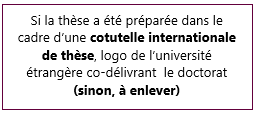
\includegraphics[scale=1]{logo2.png}

%*****************************************************
%******************** TITRE **************************
%*****************************************************

\flushright
\vspace{10mm} % à régler éventuellement
\color{Prune}
\fontfamily{cmss}\fontseries{m}\fontsize{22}{26}\selectfont
  \Huge 

\normalsize
\color{black}
~\\
\Large{Sign Language synthesis by a decreasing granularity system from AZee} \\
\small{\textit{Synthèse de langue des signes par un système d'animation à granularité décroissante à partir d'AZee}} \\
%*****************************************************

\fontfamily{fvs}\fontseries{m}\fontsize{8}{12}\selectfont

\vspace{1.5cm}

\normalsize
\textbf{Thèse de doctorat de l'université Paris-Saclay} \\

\vspace{6mm}

\small École doctorale n°580 : sciences et technologies de l’information et de la communication (STIC)\\
\small Spécialité de doctorat: informatique\\
\small Graduate School : Informatique et sciences du numérique, Référent : Faculté des sciences d’Orsay \\
\vspace{6mm}

\footnotesize Thèse préparée dans l'unité(s) de recherche \textbf{LISN} ((Université Paris-Saclay, CNRS), sous la direction de \textbf{Michael FILHOL}, Directeur de Recherche CNRS \\
\vspace{15mm}

\textbf{Thèse soutenue à Paris-Saclay, le JJ mois AAAA, par}\\
\bigskip
\Large {\color{Prune} \textbf{Paritosh SHARMA}} % Changer le Prénom et le NOM

%************************************
\vspace{\fill} % ALIGNER LE TABLEAU EN BAS DE PAGE
%************************************

\bigskip

\flushleft
\small {\color{Prune} \textbf{Composition du jury}}\\
{\color{Prune} \scriptsize {Membres du jury avec voix délibérative}} \\
\vspace{2mm}
\scriptsize
\begin{tabular}{|p{7cm}l}
\arrayrulecolor{Prune}
\textbf{Prénom NOM} &   Président ou Présidente\\ 
Titre, Affiliation & \\
\textbf{Prénom NOM} &  Rapporteur \& Examinateur / trice \\ 
Titre, Affiliation   &   \\ 
\textbf{Prénom NOM} &  Rapporteur \& Examinateur / trice \\ 
Titre, Affiliation  &   \\ 
\textbf{Prénom NOM} &  Examinateur ou Examinatrice \\ 
Titre, Affiliation   &   \\ 
\textbf{Prénom NOM} &  Examinateur ou Examinatrice \\ 
Titre, Affiliation   &   \\ 
 

\end{tabular} 

\end{titlepage}


% page des résumés à garder en 2ème page. Si les résumés sont trop longs pour tenir sur une seule et même page, on peut mettre un résumé par page
\thispagestyle{empty}
\newgeometry{top=1.5cm, bottom=1.25cm, left=2cm, right=2cm}
\fontfamily{rm}\selectfont

\lhead{}
\rhead{}
\rfoot{}
\cfoot{}
\lfoot{}

\noindent 
%*****************************************************
%***** LOGO DE L'ED À CHANGER IMPÉRATIVEMENT *********
%*****************************************************

\includegraphics[height=2.45cm]{logo_ups_EOBE.png}
\vspace{1cm}
%*****************************************************
\fontfamily{cmss}\fontseries{m}\selectfont

\small

\begin{mdframed}[linecolor=Prune,linewidth=1]

\textbf{Titre:} titre (en français)..................................................................................................................

\noindent \textbf{Mots clés:} 3 à 6 mots clefs (version en français)

\vspace{-.5cm}
\begin{multicols}{2}
\noindent \textbf{Résumé:}\lipsum[1-2] 
\end{multicols}

\end{mdframed}

\vspace{8mm}

\begin{mdframed}[linecolor=Prune,linewidth=1]

\textbf{Title:} titre (en anglais)..................................................................................................................

\noindent \textbf{Keywords:} 3 à 6 mots clefs (version en anglais)

\begin{multicols}{2}
\noindent \textbf{Abstract:} \lipsum[1-2]
\end{multicols}
\end{mdframed}

\titleformat{\chapter}[display]
{\normalfont\huge\bfseries\color{black}} % Formatting for chapter title
{\chaptertitlename\ \thechapter} % "Chapter" followed by chapter number
{20pt} % Space between "Chapter" and chapter number
{\Huge} % Formatting for chapter title
[\vspace{2ex}] % Additional space after chapter title

\titlespacing*{\chapter}{0pt}{50pt}{40pt} % Adjusting spacing around chapter title

\titleformat{\section}[hang]{\bfseries\normalsize}{\thesection\ .}{0.5pt}
{\vspace{0.1ex}
}
[\vspace{0.1ex}]
\titlespacing{\section}{1.5pc}{4ex plus .1ex minus .2ex}{.8pc}

\titleformat{\subsection}[hang]{\bfseries\small}{\thesubsection\ .}{1pt}
{\vspace{0.1ex}
}
[\vspace{0.1ex}]
\titlespacing{\subsection}{3pc}{2ex plus .1ex minus .2ex}{.1pc}

\newgeometry{top=4cm, bottom=4cm, left=2cm, right=2cm}

\tableofcontents

\newgeometry{top=4cm, bottom=4cm, left=4cm, right=4cm}

\documentclass[../../main.tex]{subfiles}
\begin{document}
\chapter{Introduction}
\label{ch:introduction}

Sign language is a primary mode of communication for the Deaf and hard-of-hearing communities, playing a crucial role in ensuring accessibility and inclusivity across various aspects of life, such as education, media, and public services. With the advancement of technology, there is an increasing need for high-quality sign language synthesis systems that can produce naturalistic and expressive animations, bridging the communication gaps between signers and non-signers.

Sign language is a rich and complex mode of communication that relies on visual-gestural modalities, utilizing hand shapes, movements, facial expressions, and body postures to convey meaning. These languages are not universal but vary across regions and cultures, each with its own grammar, syntax, and lexicon. As a result, creating effective sign language synthesis systems requires a deep understanding of both linguistic intricacies and the technical demands of real-time animation.

Despite its critical role in the lives of Deaf individuals, a significant communication gap remains between signers and non-signers, particularly in areas such as education, healthcare, media, and public services. This gap is further exacerbated by a global shortage of qualified sign language interpreters, making it difficult to provide adequate support to all who need it.

\section{Motivation}

The motivation for this research stems from the urgent need to address the challenges faced by the Deaf community in accessing essential services and engaging in daily life. Currently, sign language synthesis systems struggle to replicate the full spectrum of sign language, including the subtle nuances of hand shapes, movements, and facial expressions—elements integral to the grammar and meaning of sign language itself.

The global shortage of sign language interpreters is a well-documented issue. In Europe alone, approximately 750,000 Deaf individuals use sign language as their primary means of communication, yet there are only about 6,600 working sign language interpreters. This disparity is even greater in countries with limited resources for Deaf education and interpreter training. In many regions, the ratio of interpreters to Deaf individuals is so low that access to services is severely restricted, underscoring the importance of developing automated sign language synthesis systems as a scalable solution.

The COVID-19 pandemic has further highlighted the critical need for accessible communication, as public health information, educational content, and essential services moved online. The lack of available sign language interpreters during this time made it increasingly difficult for many Deaf individuals to access vital information, leading to a renewed focus on developing digital tools that enhance communication accessibility, particularly in virtual environments.

Advances in natural language processing, computer graphics, computer vision and machine learning  over the past decade offer promising avenues for overcoming the limitations of current sign language synthesis systems. Leveraging these technologies could lead to more advanced models capable of generating highly naturalistic and expressive sign language animations. Such models not only have the potential to improve communication for Deaf individuals but also contribute to the broader goal of creating a more inclusive society.

In addition to addressing the shortage of interpreters, there is a growing recognition of the need for cultural and linguistic diversity in sign language synthesis. Sign languages are deeply connected to the culture and identity of Deaf communities. Each sign language reflects the unique culture of its region, and any attempt to synthesize sign language must respect and preserve this diversity. This requires models that are not only technically accurate but also culturally sensitive, capable of adapting to the nuances of different sign languages while maintaining the integrity of communication.

Furthermore, sign language is highly context-dependent, with variations in signs based on factors such as the signer’s region, community, and personal style. Capturing this complexity in a digital format necessitates sophisticated models that can understand and replicate these nuances. Current systems often lack the flexibility to adapt to these variations, leading to animations that may be technically correct but lack the fluidity and expressiveness of natural sign language.

Another important motivation for this research is its potential impact on education. For Deaf students, access to educational content in sign language is crucial for academic success. However, the availability of such content is often limited, particularly in regions with few sign language interpreters. Automated sign language synthesis systems could bridge this gap, enabling the creation of educational materials that are accessible to Deaf students in their native sign language, thereby improving educational outcomes and leveling the playing field.

Finally, the increasing use of virtual environments and avatars in communication presents both challenges and opportunities for sign language synthesis. As more interactions move online, there is a growing need for avatars that can communicate in sign language with the same fluency and expressiveness as human signers. This requires advances in both animation technology and the underlying linguistic models that drive these avatars. By developing more sophisticated synthesis systems, it is possible to create avatars capable of meaningful communication with Deaf users, providing a richer and more inclusive online experience.

\section{Objectives and Contributions}

This research is centered on addressing the limitations of existing sign language synthesis systems and exploring new methods to enhance the naturalness and expressiveness of synthesized sign language animations. Specifically, this research aims to:

\begin{itemize}
    \item \textbf{Develop new methods for generating more natural and expressive sign language animations:} The focus here is on improving the quality of sign language synthesis based on linguistic input that better captures the intricacies of sign language, including hand shapes, movements, and facial expressions, which are crucial for conveying both the form and meaning of a sign language utterance.
    \item \textbf{Explore the scalability and adaptability of sign language synthesis:} Given the diversity of sign languages worldwide, it is essential to develop systems that can adapt to different linguistic and cultural contexts. This research will investigate methods to create scalable models that can be easily adapted to various sign languages and avatar systems, ensuring that the technology can be applied globally.
\end{itemize}

The contributions of this research are expected to be multifaceted, offering both theoretical and practical advancements in the field of sign language synthesis:

\begin{itemize}
    \item \textbf{Introducing novel algorithms for sign language synthesis:} This research will contribute new techniques and methodologies for synthesizing sign language, particularly in the areas of rigging, facial expression synthesis, and motion interpolation. These algorithms are designed to improve the realism and fluidity of sign language animations, making them more natural and understandable for users.
    \item \textbf{Demonstrating improvements in the realism and scalability of generated sign language:} The research will include evaluations of the proposed methods, demonstrating their effectiveness in producing sign language animations.
    \item \textbf{Providing a framework that can be adapted to various sign languages and contexts:} The ultimate goal of this research is to create a flexible and adaptable framework that can be applied to different sign languages and used in a variety of contexts, from education and media to public services.
\end{itemize}

\section{Significance of the Problem}

The significance of this research lies in its potential to close the technical gap between sign linguists and character animators, facilitating a more seamless collaboration between these fields. Traditionally, sign linguists and animators have worked in parallel but largely disconnected domains. Sign linguists focus on the linguistic structure and cultural context of sign languages, while character animators concentrate on creating visually convincing movements in digital avatars. However, the complexity and nuance of sign languages require a deeper integration of these two areas to produce animations that are both linguistically accurate and visually expressive.

One of the key innovations explored in this research is the use of the AZee framework, which provides a structured linguistic model for sign languages. AZee offers a formalism for encoding the various components of sign language, including hand shapes, movements, and facial expressions, within a unified system. By leveraging AZee, this research bridges the gap between the abstract linguistic representations of signs and the concrete visual expressions needed for character animation. This approach allows for the generation of sign language animations that are not only technically precise but also retain the fluidity and naturalness of human signing.

Moreover, AZee facilitates the creation of reusable templates and motion curves, enabling animators to produce consistent and contextually appropriate animations without needing extensive linguistic expertise. This reduces the reliance on handcrafted animations and allows for the scalability of sign language synthesis across different languages and cultural contexts. The integration of AZee into the animation pipeline enhances the adaptability of the system, making it possible to quickly generate animations for various sign languages, each with its own unique grammar and style.

In summary, the research contributes to both the field of sign language linguistics and the domain of computer animation by providing a framework that unites the strengths of both disciplines. It addresses the need for more effective tools that can translate linguistic insights into high-quality, real-time sign language animations, thus promoting greater accessibility and inclusivity for the Deaf community.

\section{Structure of the Thesis}

The structure of this thesis is designed to guide the reader through the research in a logical and coherent manner. Following this introductory chapter, Chapter~\ref{ch:background_work} provides a comprehensive review of the background work, covering existing methods in sign language synthesis, relevant techniques, and the challenges identified in the literature. This chapter sets the stage for the technical contributions that follow, offering a detailed overview of the current state of the field and the gaps that this research aims to address.

Chapter~\ref{ch:rigging_layers} introduces the concept of rigging layers, a critical component in the synthesis of sign language animations. This chapter delves into the technical aspects of creating and managing the skeletal structure of avatars, which is essential for producing realistic and fluid movements. The discussion includes both traditional and innovative approaches to rigging, highlighting the strengths and limitations of each method.

Chapter~\ref{ch:multi_track} builds on the concept of rigging by discussing the multi-track approach to sign language synthesis. This approach allows for the simultaneous representation of multiple aspects of sign language, such as hand movements, facial expressions, and body postures. By integrating these elements into a cohesive system, the multi-track approach enables the synthesis of more natural and expressive animations.

In Chapter~\ref{ch:facial_expressions}, the focus shifts to the synthesis of facial expressions, which are a critical component of sign language. Facial expressions convey a wealth of information in sign language, from grammatical markers to emotional cues. This chapter explores the challenges of synthesizing realistic facial expressions and presents new methods for integrating them into sign language animations.

Chapter~\ref{ch:intermediate_blocks} addresses the development of intermediate blocks, which are used to create smooth transitions between different elements of sign language animations. This chapter discusses the importance of motion curves and templates in achieving fluid and natural movements, and it introduces new techniques for generating intermediate blocks that enhance the overall realism of the animations.

Chapter~\ref{ch:pose_correction} focuses on motion matching techniques, which are used to ensure that the synthesized animations accurately reflect the intended sign language gestures. This chapter presents new methods for matching poses across different sign language models, with a focus on improving the accuracy and consistency of the animations.

Finally, Chapter~\ref{ch:conclusion} concludes the thesis by discussing the implications of the findings, their potential applications in real-world scenarios, and offering a summary of the key results along with suggestions for future research. This chapter also reflects on the broader impact of the research, considering how the advancements in sign language synthesis can contribute to the ongoing efforts to promote accessibility and inclusivity for Deaf individuals.

\section{Publications}

Work presented in this thesis has been the subject of the following publications:

\fullcite{sharma:hal-03721720}
\fullcite{sharma:hal-04143663}
\fullcite{10193413}
\fullcite{10.1145/3606037.3606837}
\fullcite{Sharma2024FacialEF}
\fullcite{10.1145/3658852.3659080}

\end{document}

\documentclass[../../main.tex]{subfiles}
\begin{document}
\chapter{Background Work}
\label{ch:background_work}

In this chapter, we delve into the foundational research areas central to this thesis. We begin by exploring how describing forms the basis for input into an animation system. Next, we discuss avatars as a key component of \gls{sl} synthesis. We then review the evolution of \gls{sl} descriptions, tracing their progression from linear \gls{glosses} to non-linear representations. Finally, we focus on the recent advancements in \gls{sl} synthesis, discussing various techniques and their implications for the field.

\section{Input: Sign Language Descriptions}
\label{ch:background_work:sign_language_descriptions}

A key challenge in \gls{sl} synthesis lies in the description of an \gls{sl} \gls{utterance} itself. The description of an \gls{utterance} answers essential questions such as:

\begin{itemize}
  \item \textbf{Body Motions}: What body motions create a meaningful \gls{sl} description?
  \item \textbf{Discourse Connection}: How do these motions connect to form a discourse?
  \item \textbf{Grammar and Syntax}: What are the grammatical and syntactical rules governing these signs?
  \item \textbf{\gls{non_manual_signals}}: How can \gls{non_manual_signals} (such as facial expressions and body posture) be integrated with manual signs?
\end{itemize}

In this section, we first study the descriptive languages used to formalize \gls{sl} and how they describe body motions. These descriptions are crucial as they will be the input to the \gls{sl} synthesis system.

\subsection{Lexical Approaches to Creating a Discourse}
\label{ch:background_work:sign_language_descriptions:lexical_approaches}

Lexical approaches focus on individual signs and their components, such as handshapes, movements, and locations. These are essential for understanding the building blocks of \gls{sl} and how signs are produced. Some popular lexical descriptions include:

\subsubsection{Stokoe Notation}
\label{ch:background_work:sign_language_descriptions:lexical_approaches:stokoe_notation}

Stokoe Notation~\cite{stokoe1980sign} was developed to transcribe \gls{asl}. It breaks down signs into three main components: location, handshape, and movement (figure~\ref{fig:stokoe}). It is a simple and effective notation for basic transcription but focuses primarily on the manual components of signs.

\begin{figure}[h]
  \centering 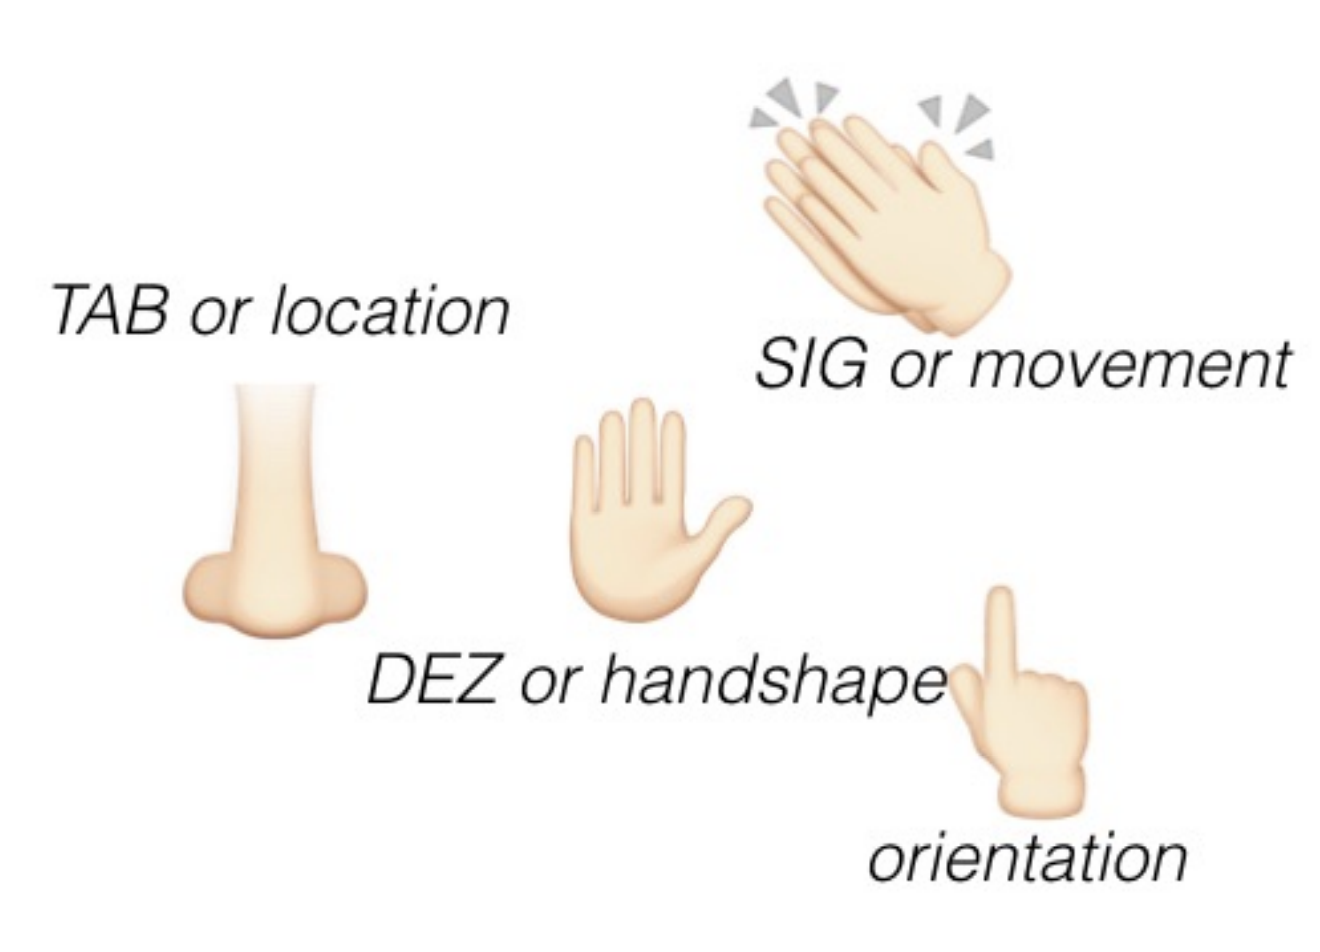
\includegraphics[width = 2.5in]{chapters/background_work/images/stokoe.png}
  \caption{Stokoe Notation}
  \label{fig:stokoe}
\end{figure}

\subsubsection{SignWriting}
\label{ch:background_work:sign_language_descriptions:lexical_approaches:signwriting}

SignWriting is a writing system developed by Valerie Sutton just after DanceWriting~\cite{sutton1973sutton} in the 1970s to represent \gls{sl} visually. It was later included as a part of the MovementWriting system. It is a featural script, representing the features of signs, such as handshapes, movements, and locations. SignWriting is designed to be easy to read and write, with symbols that resemble the gestures they represent. The script is written in two dimensions, with symbols arranged in a grid-like structure to capture various aspects of signs. Figure~\ref{fig:signwriting_coffee} shows an example of how the word "coffee" is represented in SignWriting. SignWriting has been used to transcribe over 40 \gls{sl}s worldwide and is recognized by the \gls{iswa} organization.

\begin{figure}[h]
  \centering 
\includegraphics[width = 2.5in]{chapters/background_work/images/signwriting_coffee.png}
  \caption{Coffee in SignWriting}
  \label{fig:signwriting_coffee}
\end{figure}

\subsubsection{HamNoSys}
\label{ch:background_work:sign_language_descriptions:lexical_approaches:hamnosys}

The \gls{hamnosys} is a phonetic transcription system for documenting \gls{sl}s globally, developed in 1985 at the University of Hamburg. Unlike Stokoe's notation, which was specifically created for \gls{asl}, HamNoSys aims for broader application, transcending national \gls{hamnosys} boundaries. While Stokoe notation was later adapted to other \gls{sl}s, HamNoSys was designed from the outset to accommodate the diversity found in global \gls{sl}s.

The notation system employs nearly 200 symbols, organized into five primary categories, each capturing different aspects of a sign. These categories are Handshape, Hand Orientation, Hand Location, Movement, Symmetry Operator, and Non-Manual Markers. To describe a sign, a sequence of symbols is used, with each symbol corresponding to a specific feature. The symbols are arranged in a precise order: first, Handshape, followed by Hand Orientation, Hand Location, Movement, Symmetry Operator, and finally, Non-Manual Markers. This structured sequence allows for a clear and detailed representation of the sign. Figure~\ref{fig:hamnosys_coffee} shows how the word "coffee" is represented in HamNoSys.

HamNoSys offers a detailed representation of the nuanced components in an \gls{sl} \gls{utterance} rather than serving as a practical writing system. Its main purpose is linguistic, used primarily by linguists to analyze the specific features of individual signs. However, it has also found its applications in synthesis~\cite{elliott2010towards} as well as sign detection~\cite{mocialov2022unsupervised}.

\begin{figure}[h]
  \centering 
\includegraphics[width = 2.5in]{chapters/background_work/images/hamnosys_coffee.png}
  \caption{Coffee in HamNoSys}
  \label{fig:hamnosys_coffee}
\end{figure}

\subsection{AZee}
\label{ch:background_work:sign_language_descriptions:azee}

Even though these previously discussed lexical approaches are effective in capturing the individual components of signs, they are limited in their ability to represent the dynamic and context-sensitive nature of \gls{sl} discourse. This is because they simplify signs as \gls{glosses}. As a reason, their applications in \gls{sl} synthesis are limited. The AZee model, however, is grounded in the concept of production rules, which link specific meanings to observable forms. This model operates on the principle that the meaning of a sign can be broken down into a set of features, which are then represented through production rules. These rules guide the generation of the sign's form, encompassing aspects like handshape, movement, and location. Designed to be both flexible and extensible, the AZee model is capable of representing a broad spectrum of signs and \gls{sl}s. It is particularly advantageous for \gls{sl} synthesis, offering a systematic and structured method for describing signs and their components.

\subsubsection{Representation of an \gls{utterance} in AZee}
\label{ch:background_work:sign_language_descriptions:azee:representation}

The AZee model uses a hierarchical structure to represent signs, with each level capturing different aspects of the sign. At the lowest level, the model describes the physical form of the sign, such as handshapes, movements, and locations. These physical forms are then combined to create more complex signs, forming a hierarchical structure that mirrors the linguistic structure of the sign. To understand this better, consider the example of the \gls{utterance} "a person aged 52" in \gls{lsf} from the \emph{1R-JP} discourse from the 40 brèves corpus~\cite{challant2022first}. The AZee code for this \gls{utterance} would be:

\begin{verbatim}
  :info-about
    'topic
    :personne
    'info
    :info-about
      'topic
      :âge
      'info
      :tens-units
        'tens
        .nb-5
        'units
        .nb-2
\end{verbatim}

The \gls{azee_interpreter} parses this description recursively, generating an \gls{azee_score}. An \gls{azee_score} being recursive in nature can contain other \gls{azee_score}s. The figure~\ref{fig:azee_score_example} shows the recursive structure for the \gls{utterance} "a person aged 52" using the AZee model. Each of the blocks in the figure represents an \gls{azee_score} .

\begin{figure}[h]
  \centering 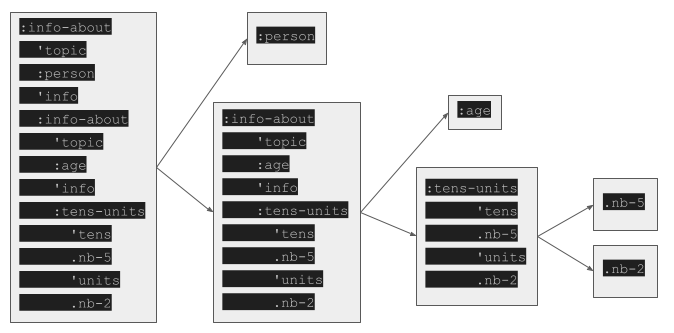
\includegraphics[width = 5in]{chapters/background_work/images/azee_score_example.png}
  \caption{AZee's recursive score representation for the utterance "a person aged 52"}
  \label{fig:azee_score_example}
\end{figure}

Note that the \gls{azee_score} representation also gives us temporal information about the \gls{utterance}. Such a detailed representation is important to us as it can help in creation of a timeline and will also be the input for our \gls{sl} synthesis system. 

\subsubsection{Low-Level Descriptions in AZee}
\label{ch:background_work:sign_language_descriptions:azee:low_level}

Apart from the high-level representation of an \gls{utterance} as shown in figure ~\ref{fig:azee_score_example}, the AZee model also supports low-level descriptions that directly correlate with the postures of an abstract avatar. This low-level description is also a recursive \gls{azee_score} and contains a set of \gls{cstr_score}s. A \gls{cstr_score} is a score which contains a set of \gls{posture_constraint}s on the posture that capture various components of the utterance, such as handshapes, movements, and locations. For example, let's consider the \gls{azee_score} for \emph{:personne} (person in \gls{lsf}, figure~\ref{fig:person_lsf}) in the above utterance. Figure ~\ref{fig:azee_score_person} shows the low-level description for this \gls{azee_score}. It contains 4 \gls{cstr_score}s, \emph{HAND\_START}, \emph{HAND\_END}, \emph{HAND\_PATH}, and \emph{PERM}, each containing \gls{posture_constraint}s on the posture of the avatar.

\begin{figure}
  \centering 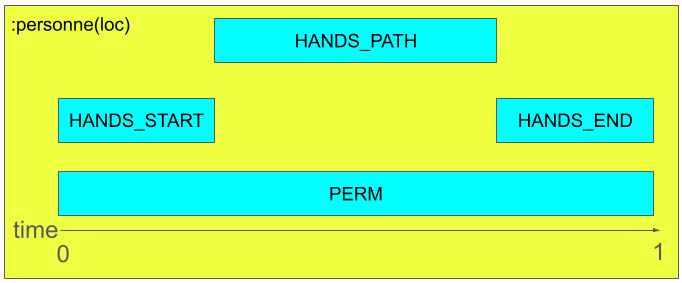
\includegraphics[width = 4in]{chapters/background_work/images/azee_score_person.png}
  \caption{Low-level description for \emph{:personne}}
  \label{fig:azee_score_person}
\end{figure}

\begin{figure}
  \centering 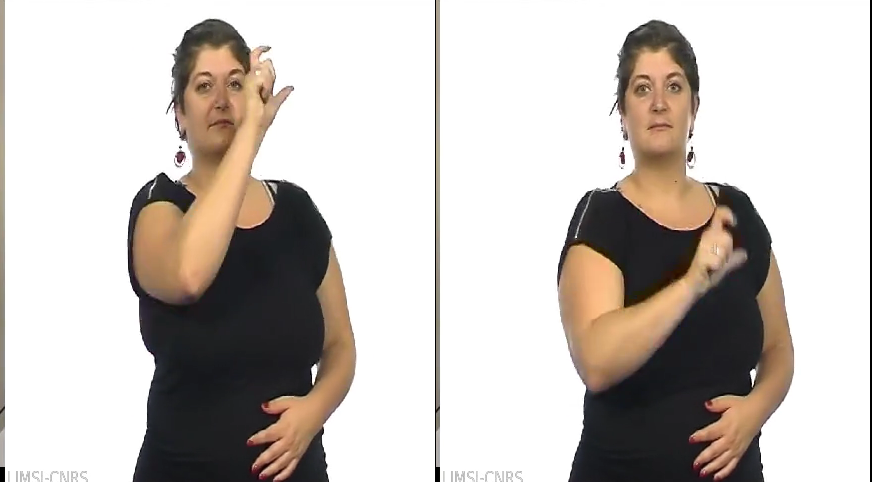
\includegraphics[width = 3.5in]{chapters/background_work/images/person_lsf.png}
  \caption{Person in French Sign Language}
  \label{fig:person_lsf}
\end{figure}

\emph{HAND\_START} and \emph{HAND\_END} represent the hands placements and orientations at the start and end of the sign, respectively. \emph{HAND\_PATH} captures the trajectory of the head during the sign, while \emph{PERM} contains the permanent features which are active throughout the duration (in this case, closed middle, ring and pinky fingers while the thumb and index are partially open).

An \gls{azee_score} can be of various types. These include:

\begin{itemize}
  \item \textbf{Synced Score}: A recrusive structure containing other scores with some sync rules (relative timing information of the underlying scores) (figure~\ref{fig:azee_score_example}).
  \item \textbf{\gls{cstr_score}}: A score specifying \gls{posture_constraint}s on the body parts (figure~\ref{fig:azee_score_person}).
  \item \textbf{Hold Score}: A score holding another score for some amount of time.
  \item \textbf{KeyFrame Score}: An abstract \emph{flattened} representation of a \gls{cstr_score}.
  \item \textbf{Non-Animated KeyFrame Score}: A \emph{flattened} representation of \gls{posture_constraint}s on body parts per frame.
  \item \textbf{Animated KeyFrame Score}: A \emph{flattened} representation of pose changes per frame.
\end{itemize}

Similarly, \gls{posture_constraint}s in a \gls{cstr_score} can be of various types. These include:

\begin{itemize}
  \item \textbf{Place}: Constrains a body \gls{site} to be placed at a specific location in 3D space.
  \item \textbf{Orient}: Constraints the orientation of a bone.
  \item \textbf{Morph}: Constrains a morphological change of a body part(s).
  \item \textbf{Transpath}: Constrains a body \gls{site} along a path.
  \item \textbf{Look-At}: Constrains the body to look at a specific point.
  \item \textbf{Trill}: Shaking of a body part along an axis.
\end{itemize}

In addition to these, the AZee model includes several other important operators and concepts that allows to represent \gls{sl}. Some of these include,

\begin{itemize}
  \item \textbf{Dynamic Points and Paths}: to define moving targets or locations that body parts should follow.
  \item \textbf{3D math operations}: Various math operations such as vectors, mathematical curves, and transformations are supported in AZee.
  \item \textbf{Partial Application of Operators}: allows for the partial application of an operator to a set of arguments, effectively creating a new operator.
\end{itemize}

\subsubsection{AZee Templates}
\label{ch:background_work:sign_language_descriptions:azee:templates}

AZee also allows for use of templates which help us identifying patterns in a \gls{sl} utterance, linking linguistic descriptions with animated motions. For example, an AZee template like \emph{:info-about(:âge,?info)} could match an AZee expression such as \emph{:info-about(:âge,:tens-units(:five,:two))}, where the variable \emph{info} would be assigned the function \emph{:tens-units(:five,:two)}. This template can be used to procedurally create animations, where the person's age (52, in this case) is dynamically inserted based on the template match.

Lastly, an AZee description can also be drawn in the form of \gls{svg} images using \gls{azvd}~\cite{filhol2024software}. Figure~\ref{fig:azvd} shows the verbalizing diagrams for the \gls{utterance} "a person aged 52".

\begin{figure}
  \centering 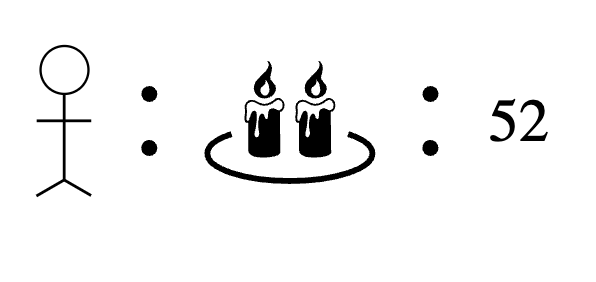
\includegraphics[width = 2.5in]{chapters/background_work/images/azvd.png}
  \caption{AZVD for a person aged 52}
  \label{fig:azvd}
\end{figure}

Since AZee representes \gls{sl} in a structured and hierarchical manner with much more detail, we choose to use it as the input for our \gls{sl} synthesis system.

\section{Sign Language Synthesis}
\label{ch:background_work:sign_language_synthesis}

\gls{sl} synthesis is the process of generating \gls{sl} discourses from linguistic input. This process involves resolving a linguistic description on a digital human. This can be in the form of handshapes, movements, facial expressions, etc. \gls{sl} synthesis is a complex and interdisciplinary field that draws on linguistics, computer science, animation, and human-computer interaction. Several approaches have been developed to synthesize \gls{sl} animations, each with its unique strengths and challenges.

\subsection{2D Techniques}
\label{ch:background_work:sign_language_synthesis:2d_techniques}

Various 2D synthesis~\cite{jiang2024signclipconnectingtextsign, moryossef2024signmtrealtimemultilingualsign} already exist which generate signs directly from \gls{glosses}. One of the newer techniques~\cite{walsh2024sign} addresses the common issue of regression to the mean in previous models, which often resulted in unnatural and under-articulated signing. The authors propose a method called "sign stitching," which involves normalizing signs into a canonical pose, cropping, stitching them together, and applying frequency domain filtering and resampling to produce cohesive, expressive \gls{sl} sequences. They also introduce a \gls{nsvq} transformer to integrate facial expressions, enhancing the naturalness of the signs. The approach is evaluated using a SignGAN model~\cite{saunders2020everybodysignnowtranslating} to generate photo-realistic signers, achieving state-of-the-art performance across multiple datasets and receiving positive feedback in user evaluations for its realism and expressiveness.

Figures~\ref{fig:synthesis_mediaipe_2d} and~\ref{fig:synthesis_gan_2d} illustrate how the output of such methods usually look like, showing the initial mediapipe-based synthesis and the subsequent fitting of a GAN on the Mediapipe skeleton to enhance the realism of the generated signs.

\begin{figure}
  \centering 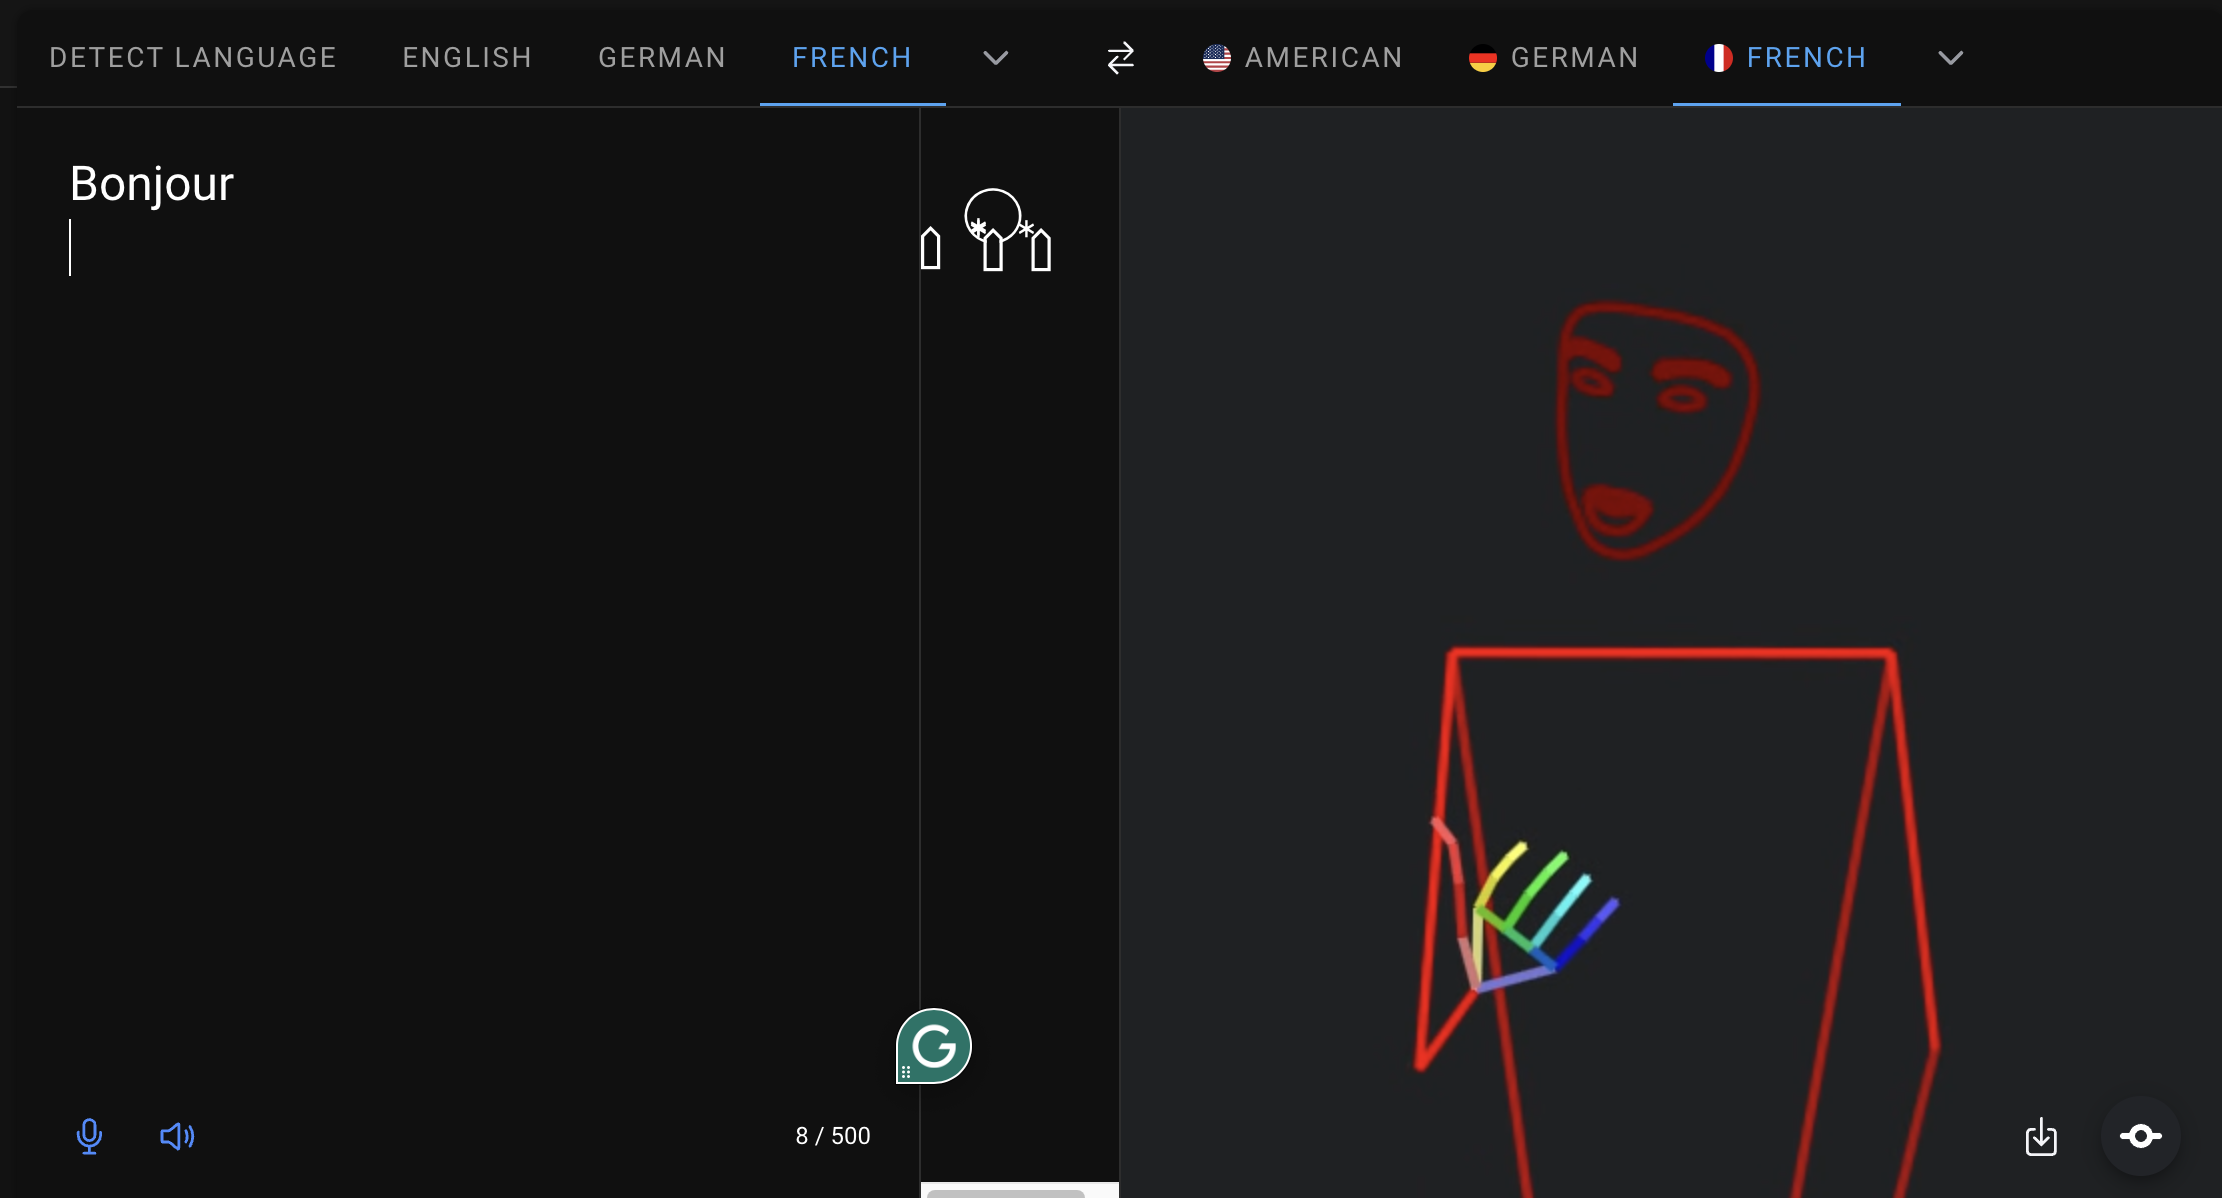
\includegraphics[width = 2.5in]{chapters/background_work/images/sign_writing_synthesis.png} 
  \caption{Synthesis using Sign-Stitching} 
  \label{fig:synthesis_mediaipe_2d} 
\end{figure}

\begin{figure} 
  \centering 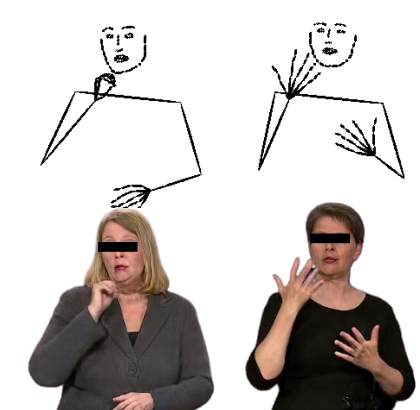
\includegraphics[width = 2.5in]{chapters/background_work/images/gan_synthesis.png} 
  \caption{SignGAN~\cite{saunders2020everybodysignnowtranslating}} 
  \label{fig:synthesis_gan_2d} 
\end{figure}

While such techniques are computationally less demanding during inference. Require a large amount of data to train the model. They also lack the depth and realism of 3D animations and struggle with capturing complex spatial relationships in \gls{sl}.

\subsection{3D Techniques}
\label{ch:background_work:sign_language_synthesis:3d_techniques}

3D techniques generate \gls{sl} animations using avatars that operate in a three-dimensional space. These methods provide a more immersive and realistic representation of \gls{sl}. 3D synthesis can leverage advanced avatars, such as those created by MetaHuman or SMPL-X, to achieve high levels of detail and expressiveness. Avatars are digital representations of characters or individuals, and are quite poular in in \gls{sl} synthesis to animate the described signs. This subsection explores the components of avatar creation and animation, followed by their use in \gls{sl} synthesis.

\subsubsection{Skeleton}
\label{ch:background_work:sign_language_synthesis:3d_techniques:skeleton}

The skeleton of a digital avatar is a crucial component for enabling realistic movement and animation. It consists of a hierarchical structure of bones, joints that mimic the human skeletal system. This section explores several popular skeleton systems used in avatar creation and animation.

\paragraph{Mixamo}
\label{ch:background_work:sign_language_synthesis:3d_techniques:skeleton:mixamo}

Mixamo is a widely used online platform that provides a vast library of pre-rigged 3D characters and animations. Developed by Adobe, Mixamo offers an easy-to-use interface where users can upload their 3D models and automatically rig(add skeleton and other controllable features) them using Mixamo's auto-rigging tool. This tool identifies keypoints on the model and generates a skeleton with appropriate bone placements. Additionally, Mixamo offers a range of pre-made animations that can be applied to the rigged models, facilitating quick and efficient animation workflows. The platform supports various file formats and is compatible with many 3D software tools. A standard Mixamo skeleton consists of 65 bones, covering major body parts, including the spine, arms, legs, hands, and head. Figure~\ref{fig:mixamo_autorigging} shows the process of auto-rigging a 3D model using Mixamo, while Figure~\ref{fig:mixamo_skeleton} illustrates the standard Mixamo skeleton structure.

\begin{figure} 
  \centering 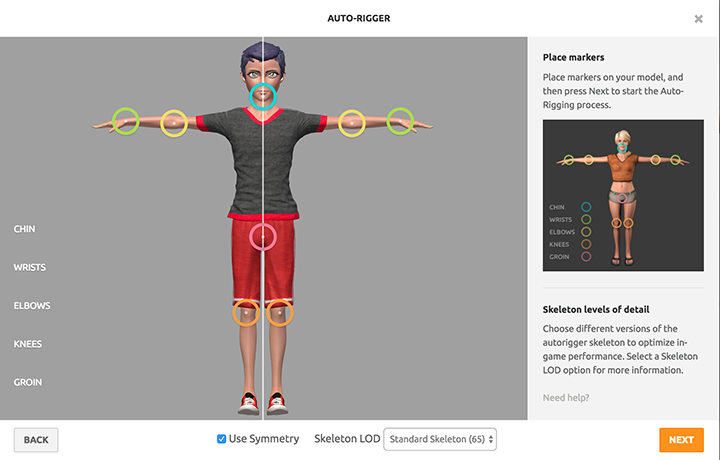
\includegraphics[width = 2.5in]{chapters/background_work/images/mixamo_autorigging.png} 
  \caption{Autorigging using Mixamo} 
  \label{fig:mixamo_autorigging} 
\end{figure}

\begin{figure} 
  \centering 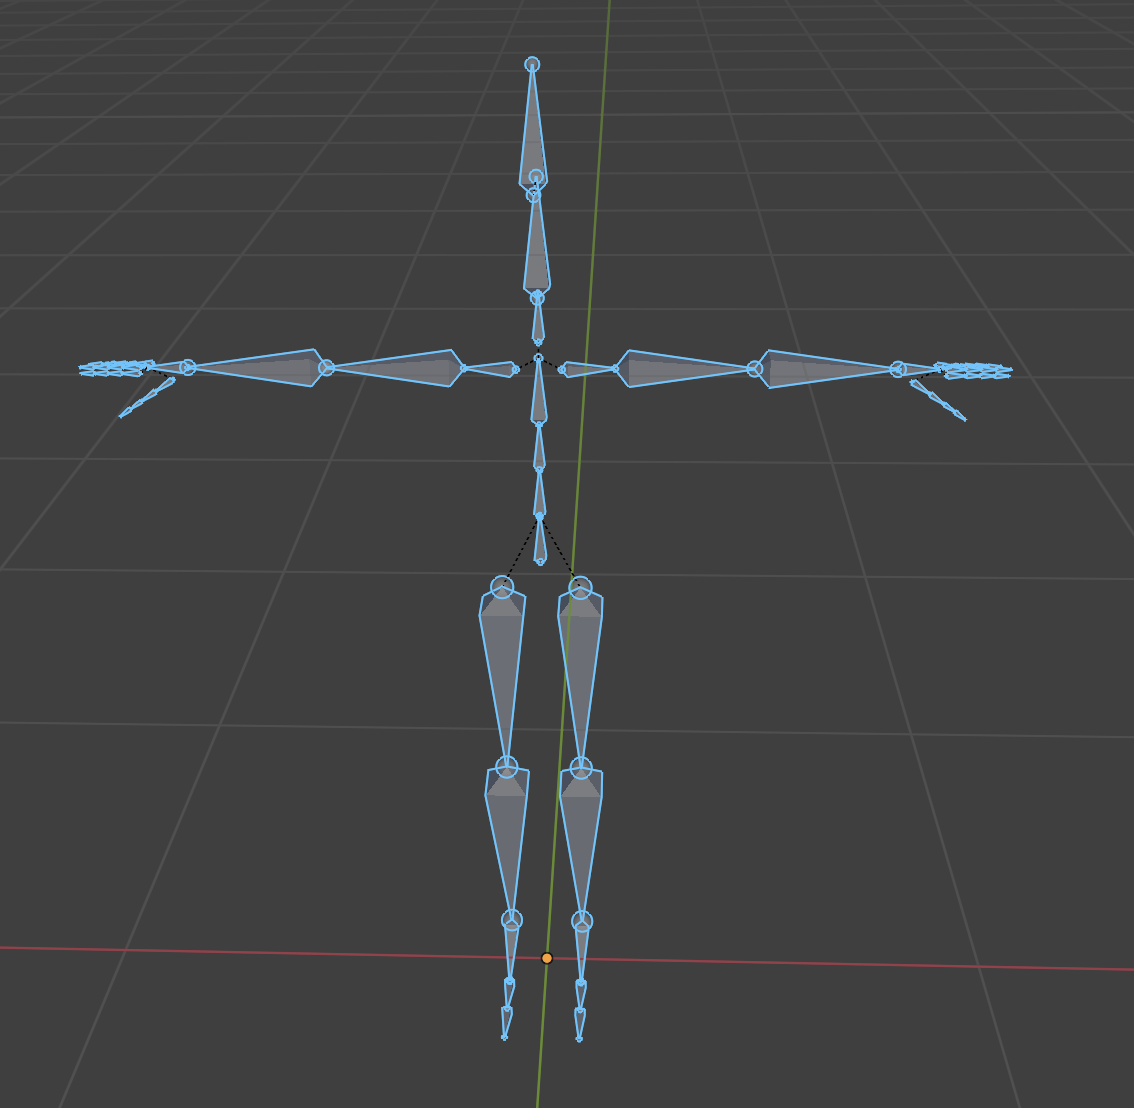
\includegraphics[width = 2.5in]{chapters/background_work/images/mixamo_skeleton.png} 
  \caption{Standard Mixamo skeleton structure} 
  \label{fig:mixamo_skeleton} 
\end{figure}

\paragraph{SMPL-X}
\label{ch:background_work:sign_language_synthesis:3d_techniques:skeleton:smpl_x}

\gls{smplx} is a state-of-the-art parametric model for generating highly detailed and anatomically accurate 3D human avatars. SMPL-X encodes the shape and pose of a character using a low-dimensional space, allowing for efficient representation and manipulation. Thus, a configuration of about 100 numbers can represent the pose as well as the shape of the avatar. The hierarchy of a SMPL-X skeleton is shown in figure~\ref{fig:smpl_x_skeleton}, and the corresponding \gls{latent_space} representation in figure~\ref{fig:latent_space_smplx}.

\begin{figure} 
  \centering 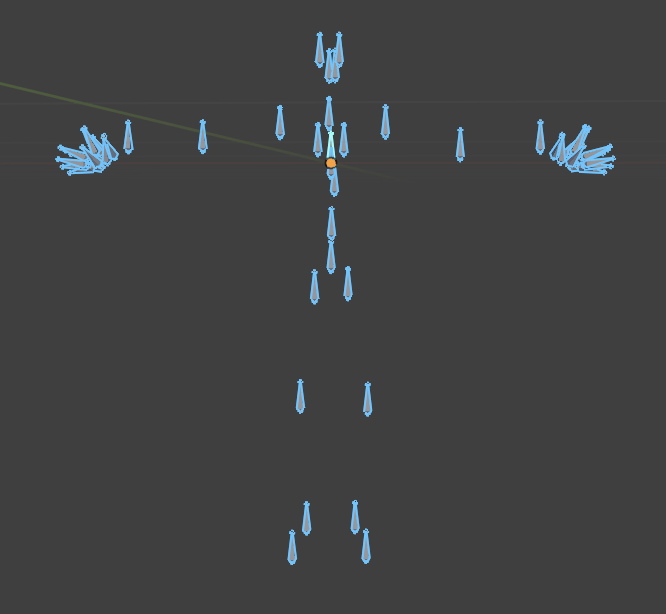
\includegraphics[width = 2.5in]{chapters/background_work/images/smpl_x_skeleton.png} 
  \caption{SMPL-X skeleton} 
  \label{fig:smpl_x_skeleton} 
\end{figure}

\begin{figure} 
  \centering 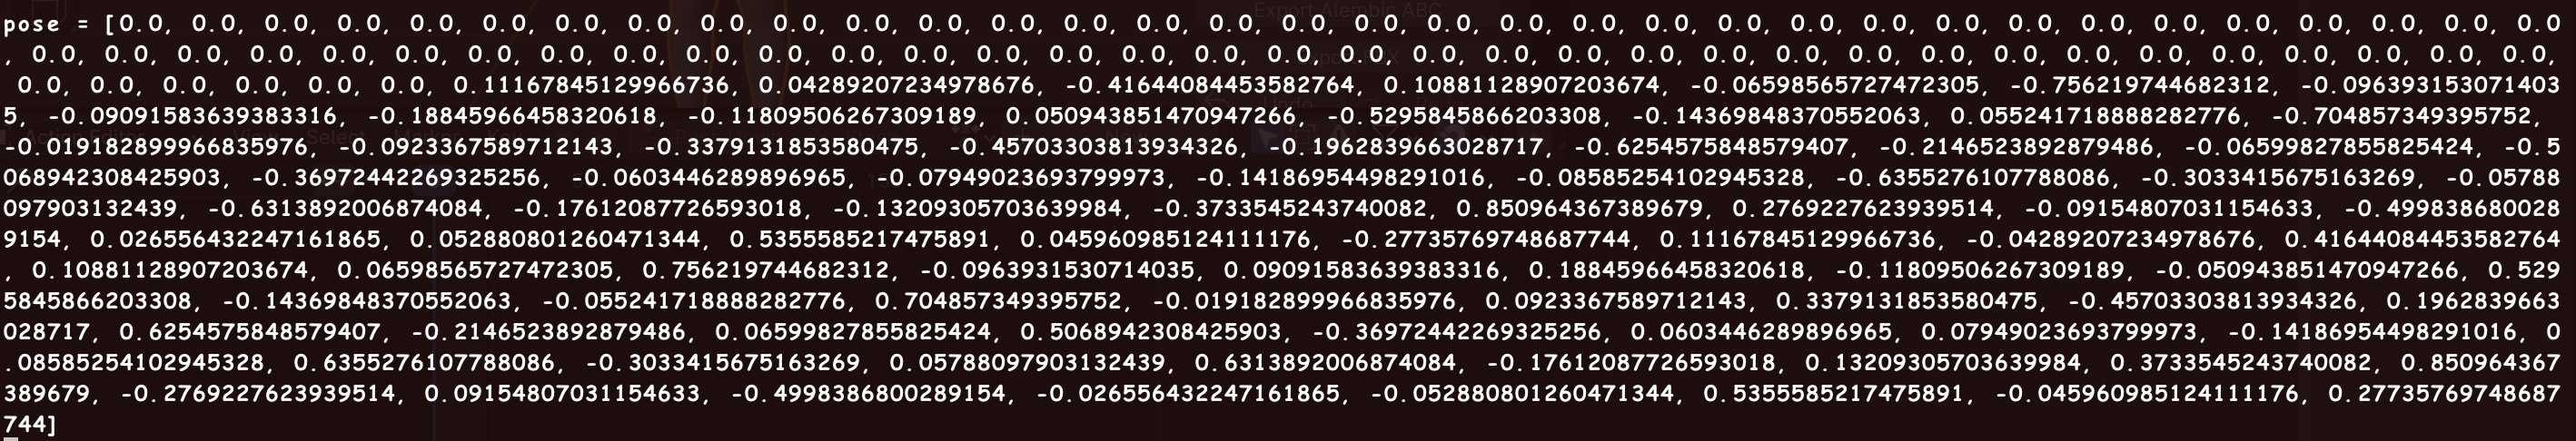
\includegraphics[width = 2.5in]{chapters/background_work/images/latent_space_smplx.png} 
  \caption{SMPL-X latent space} 
  \label{fig:latent_space_smplx} 
\end{figure}

\subsubsection{Mesh and Texture}
\label{ch:background_work:sign_language_synthesis:3d_techniques:mesh_and_texture}

The mesh of a digital avatar is the 3D model that forms the surface representation of the character. It consists of vertices, edges, and faces that define the shape and structure of the avatar. Creating and manipulating meshes is a fundamental aspect of 3D modeling and animation, allowing for detailed and realistic character designs.

Textures are 2D images applied to the surface of a 3D model to enhance its appearance and realism. Textures can represent various surface properties such as color, roughness, reflectivity, and transparency. Common types of textures include diffuse maps (color), specular maps (reflectivity), normal maps (surface detail), and roughness maps (surface smoothness). By combining different textures, artists can create visually compelling avatars with intricate surface details and lifelike appearances. These textures are often mapped onto the mesh of the avatar using UV mapping techniques to ensure proper alignment and scaling.

\paragraph{Weight Painting}
\label{ch:background_work:sign_language_synthesis:3d_techniques:mesh_and_texture:weight_painting}

Weight painting is a technique used to define how much influence each bone in a skeleton has over the surrounding mesh vertices. It plays a crucial role in ensuring that the mesh deforms naturally and realistically when the skeleton is animated. Figure~\ref{fig:weight_painting} shows an example of weight painting in Blender, with the red color indicating high influence and blue indicating low influence.

\begin{figure} 
  \centering 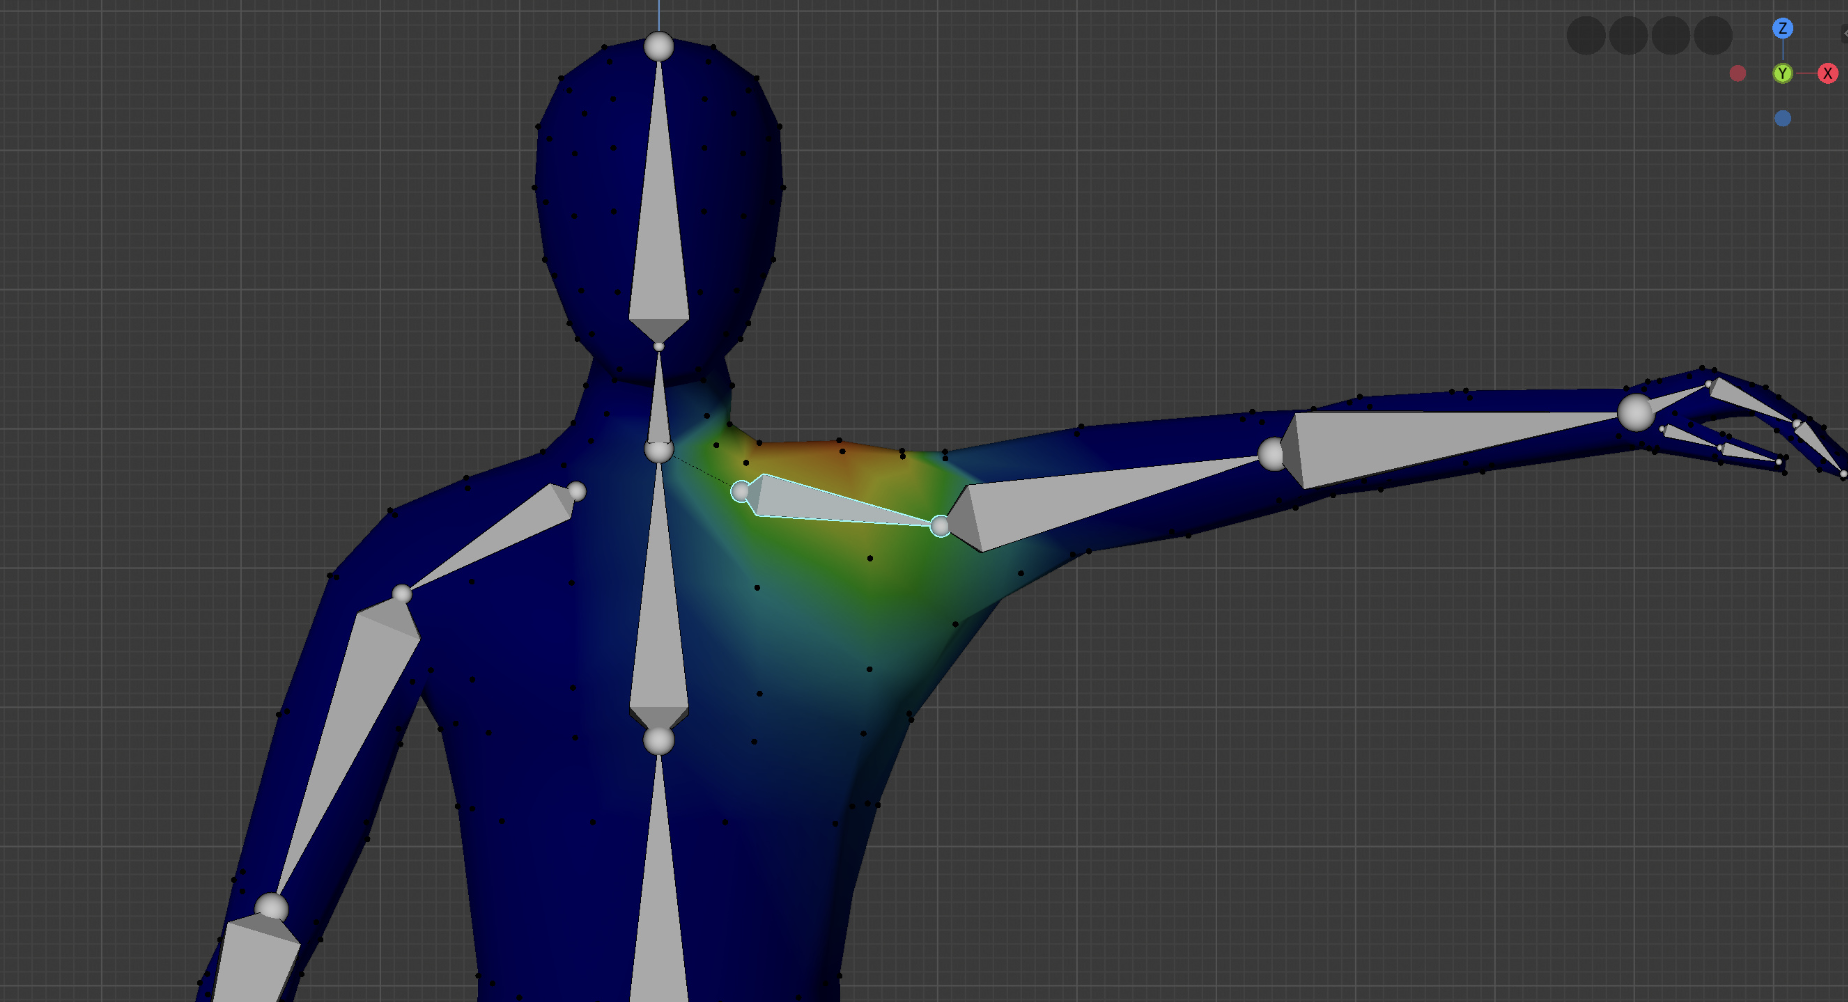
\includegraphics[width = 2.5in]{chapters/background_work/images/weight_painting.png} 
  \caption{Weight painting in Blender} 
  \label{fig:weight_painting} 
\end{figure}

\subsubsection{Rigging}
\label{ch:background_work:sign_language_synthesis:3d_techniques:rigging}

A rig is the final system used by the artists to animate the avatars. This is done by implementing all the above systems in order, i.e., creating a skeleton, mesh, texture, weight painting, facial blendshapes, implementing \gls{ik} and \gls{fk} systems, and adding constraints. Figure~\ref{fig:rig_example} shows an example of a rigged character, the "Rain rig" by Blender Studio.

\begin{figure} 
  \centering 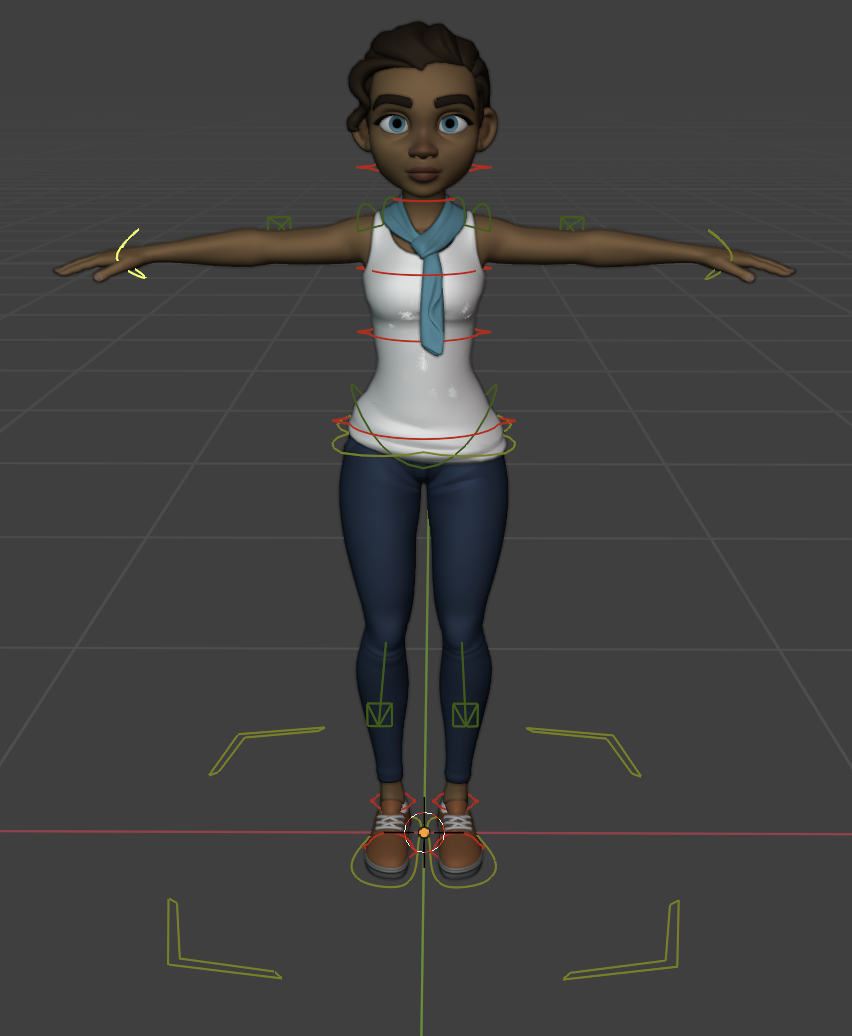
\includegraphics[width = 2.5in]{chapters/background_work/images/rig_example.png} 
  \caption{Rain rig by Blender studio} 
  \label{fig:rig_example} 
\end{figure}

\subsubsection{Procedural Avatar Creation}
\label{ch:background_work:sign_language_synthesis:3d_techniques:procedural_avatar_creation}

Procedural avatar creation involves the use of algorithms and software tools to automatically generate 3D characters with minimal manual intervention. This approach can significantly speed up the character creation process since it automates the creation of all of the avatar components discussed above. This allows rapid development of detailed and diverse avatars. This section explores several prominent tools and models used for procedural avatar creation.

\paragraph{MakeHuman}
\label{ch:background_work:sign_language_synthesis:3d_techniques:procedural_avatar_creation:makehuman}

MakeHuman is an open-source tool specifically designed for the rapid prototyping of humanoid avatars. It allows users to create 3D human models through an intuitive interface where parameters such as gender, age, ethnicity, and body proportions can be adjusted using sliders. Figure~\ref{fig:makehuman_example} demonstrates the process of creating an avatar using MakeHuman.

\begin{figure} 
  \centering 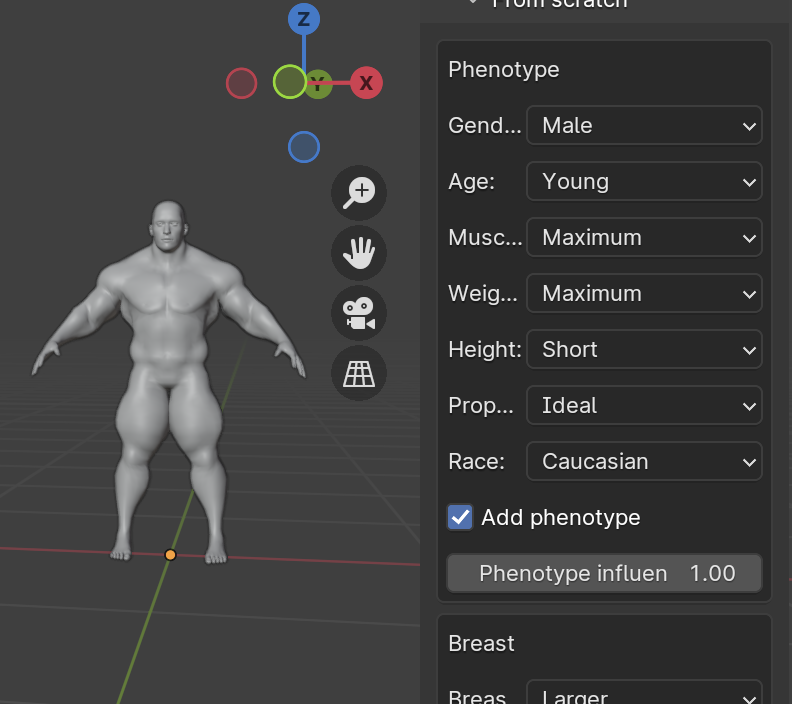
\includegraphics[width = 2.5in]{chapters/background_work/images/makehuman_example.png} 
  \caption{Avatar creation using MakeHuman} 
  \label{fig:makehuman_example} 
\end{figure}

\paragraph{SMPL-X or Meshcapade}
\label{ch:background_work:sign_language_synthesis:3d_techniques:procedural_avatar_creation:smpl_x_meshcapade}

Just like MakeHuman, SMPL-X can create avatars with parameters such as weight, height, age, etc. However, SMPL-X can also be created using images of a person. This allows it to be more realistic than MakeHuman. Figure~\ref{fig:smpl_creation_example} shows the process of creating an SMPL-X avatar using the Meshcapade tool.

\begin{figure} 
  \centering 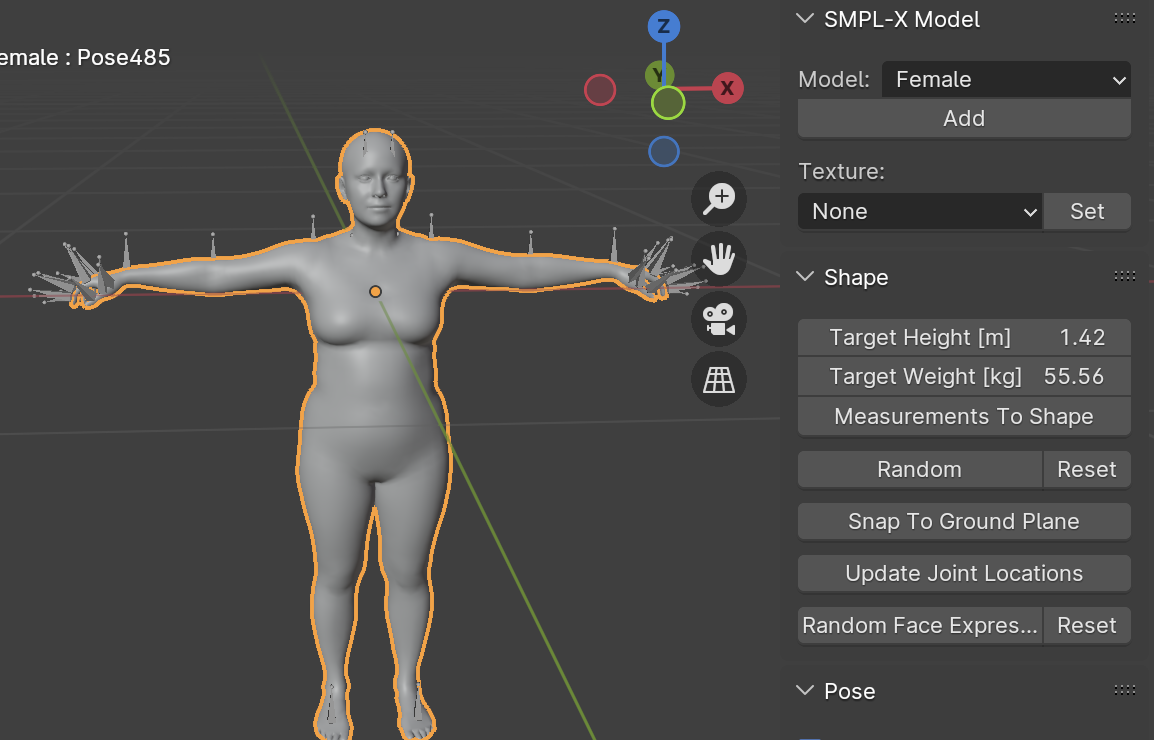
\includegraphics[width = 2.5in]{chapters/background_work/images/smpl_creation_example.png} 
  \caption{SMPL-X avatar creation using Meshcapade} 
  \label{fig:smpl_creation_example} 
\end{figure}

\paragraph{MetaHuman}
\label{ch:background_work:sign_language_synthesis:3d_techniques:procedural_avatar_creation:metahuman}

MetaHuman Creator (figure~\ref{fig:metahuman_example}), developed by Epic Games, is a tool for creating ultra-realistic digital humans. The tool's emphasis on realism and detail makes it a powerful resource for creating lifelike characters for games, films, and other interactive experiences. MetaHumans are the most realistic avatars available today, with high-quality textures, detailed facial expressions, and advanced animation controls.

\begin{figure} 
  \centering 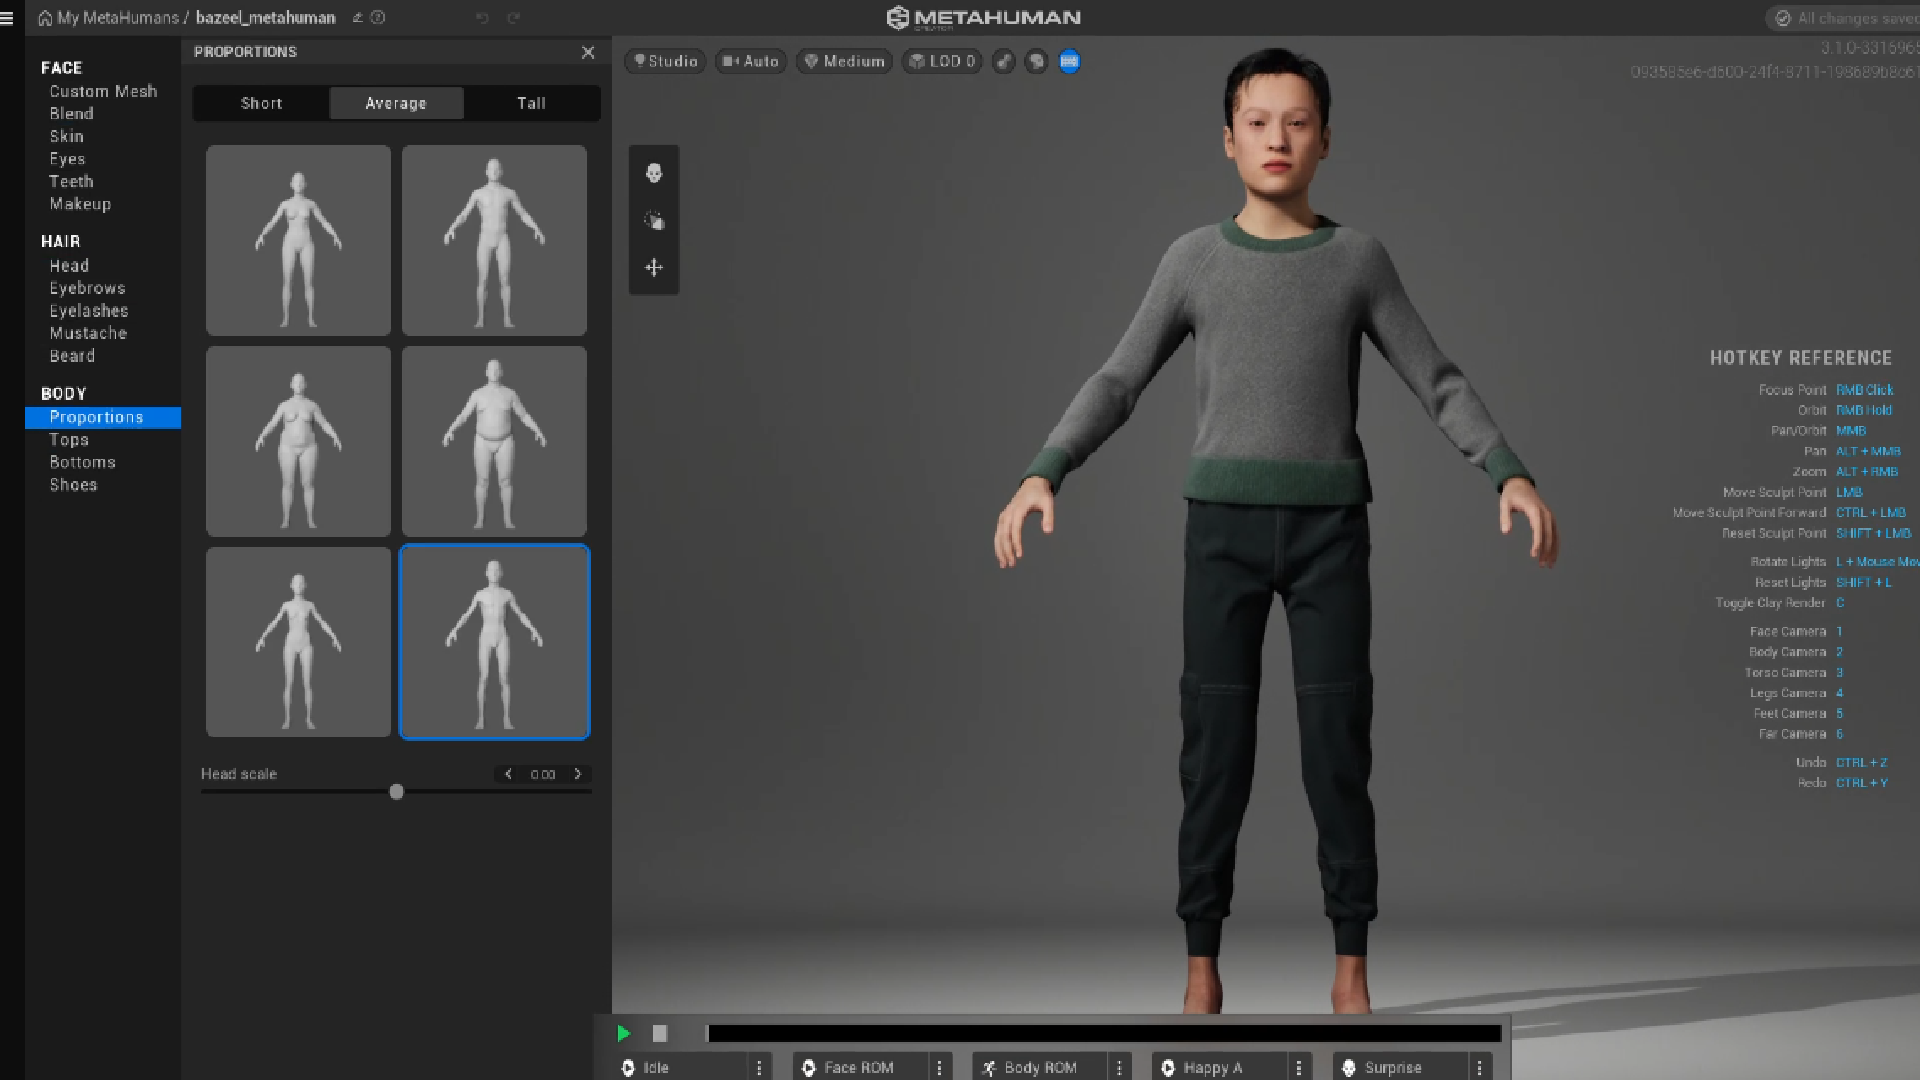
\includegraphics[width = 2.5in]{chapters/background_work/images/metahuman_example.png} 
  \caption{Avatar creation using MetaHuman} 
  \label{fig:metahuman_example}
\end{figure}

\subsubsection{Avatar Animation}
\label{ch:background_work:sign_language_synthesis:3d_techniques:avatar_animation}

The methods used for animating avatars range from manual to automated processes, each offering unique benefits and challenges. This section explores the key methods used in avatar animation.

\paragraph{Manual Keyframing}
\label{ch:background_work:sign_language_synthesis:3d_techniques:avatar_animation:manual_keyframing}

Manual keyframing is a traditional animation technique where animators define specific poses, known as keyframes, at critical points in time. These keyframes mark the start and end points of any smooth transition or movement. The intermediate poses are then calculated using interpolation. This method provides animators with precise control over every aspect of the avatar’s movement, making it ideal for achieving nuanced and detailed animations.

Figure~\ref{fig:keyframing} shows the process of manual keyframing to animate a sprite.

\begin{figure} 
  \centering 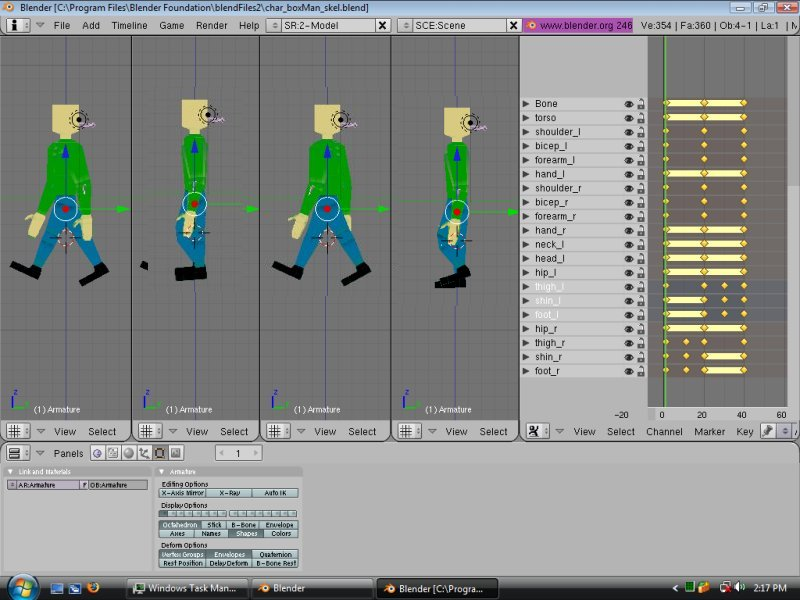
\includegraphics[width = 2.5in]{chapters/background_work/images/keyframing.png} 
  \caption{Manual keyframing to animate a sprite} 
  \label{fig:keyframing} 
\end{figure}

Along with keyframing, motion curves~\cite{10.1145/218380.218422} are used to control the interpolation between keyframes. These curves define the speed and timing of the animation, allowing animators to create smooth and natural movements. Common types of motion curves include linear, ease-in, ease-out, and bezier curves. By adjusting the shape and slope of these curves, animators can fine-tune the animation to achieve the desired effect. Figure~\ref{fig:motion_curves} shows examples of different motion curves used to fine-tune an animation.

\begin{figure} 
  \centering 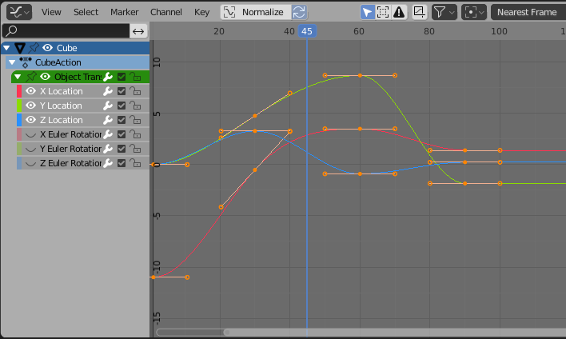
\includegraphics[width = 2.5in]{chapters/background_work/images/motion_curves.png} 
  \caption{Motion curves to finetune an animation} 
  \label{fig:motion_curves} 
\end{figure}

\paragraph{Mocap Retargeting}
\label{ch:background_work:sign_language_synthesis:3d_techniques:avatar_animation:mocap_retargeting}

Motion capture (mocap) retargeting involves capturing the movements of a real human actor and applying this data to a digital avatar. This process starts with recording an actor’s performance using a motion capture system, which tracks the actor’s movements through markers or sensors placed on their body. The recorded data is then mapped onto the avatar’s skeleton, a process known as retargeting. Mocap retargeting ensures highly realistic animations by directly transferring the nuances of human motion to the digital character. This technique is widely used in the entertainment industry, particularly in video games and films, to create lifelike animations.

Figure~\ref{fig:mocap} illustrates the process of motion capture and retargeting.

\begin{figure} 
  \centering 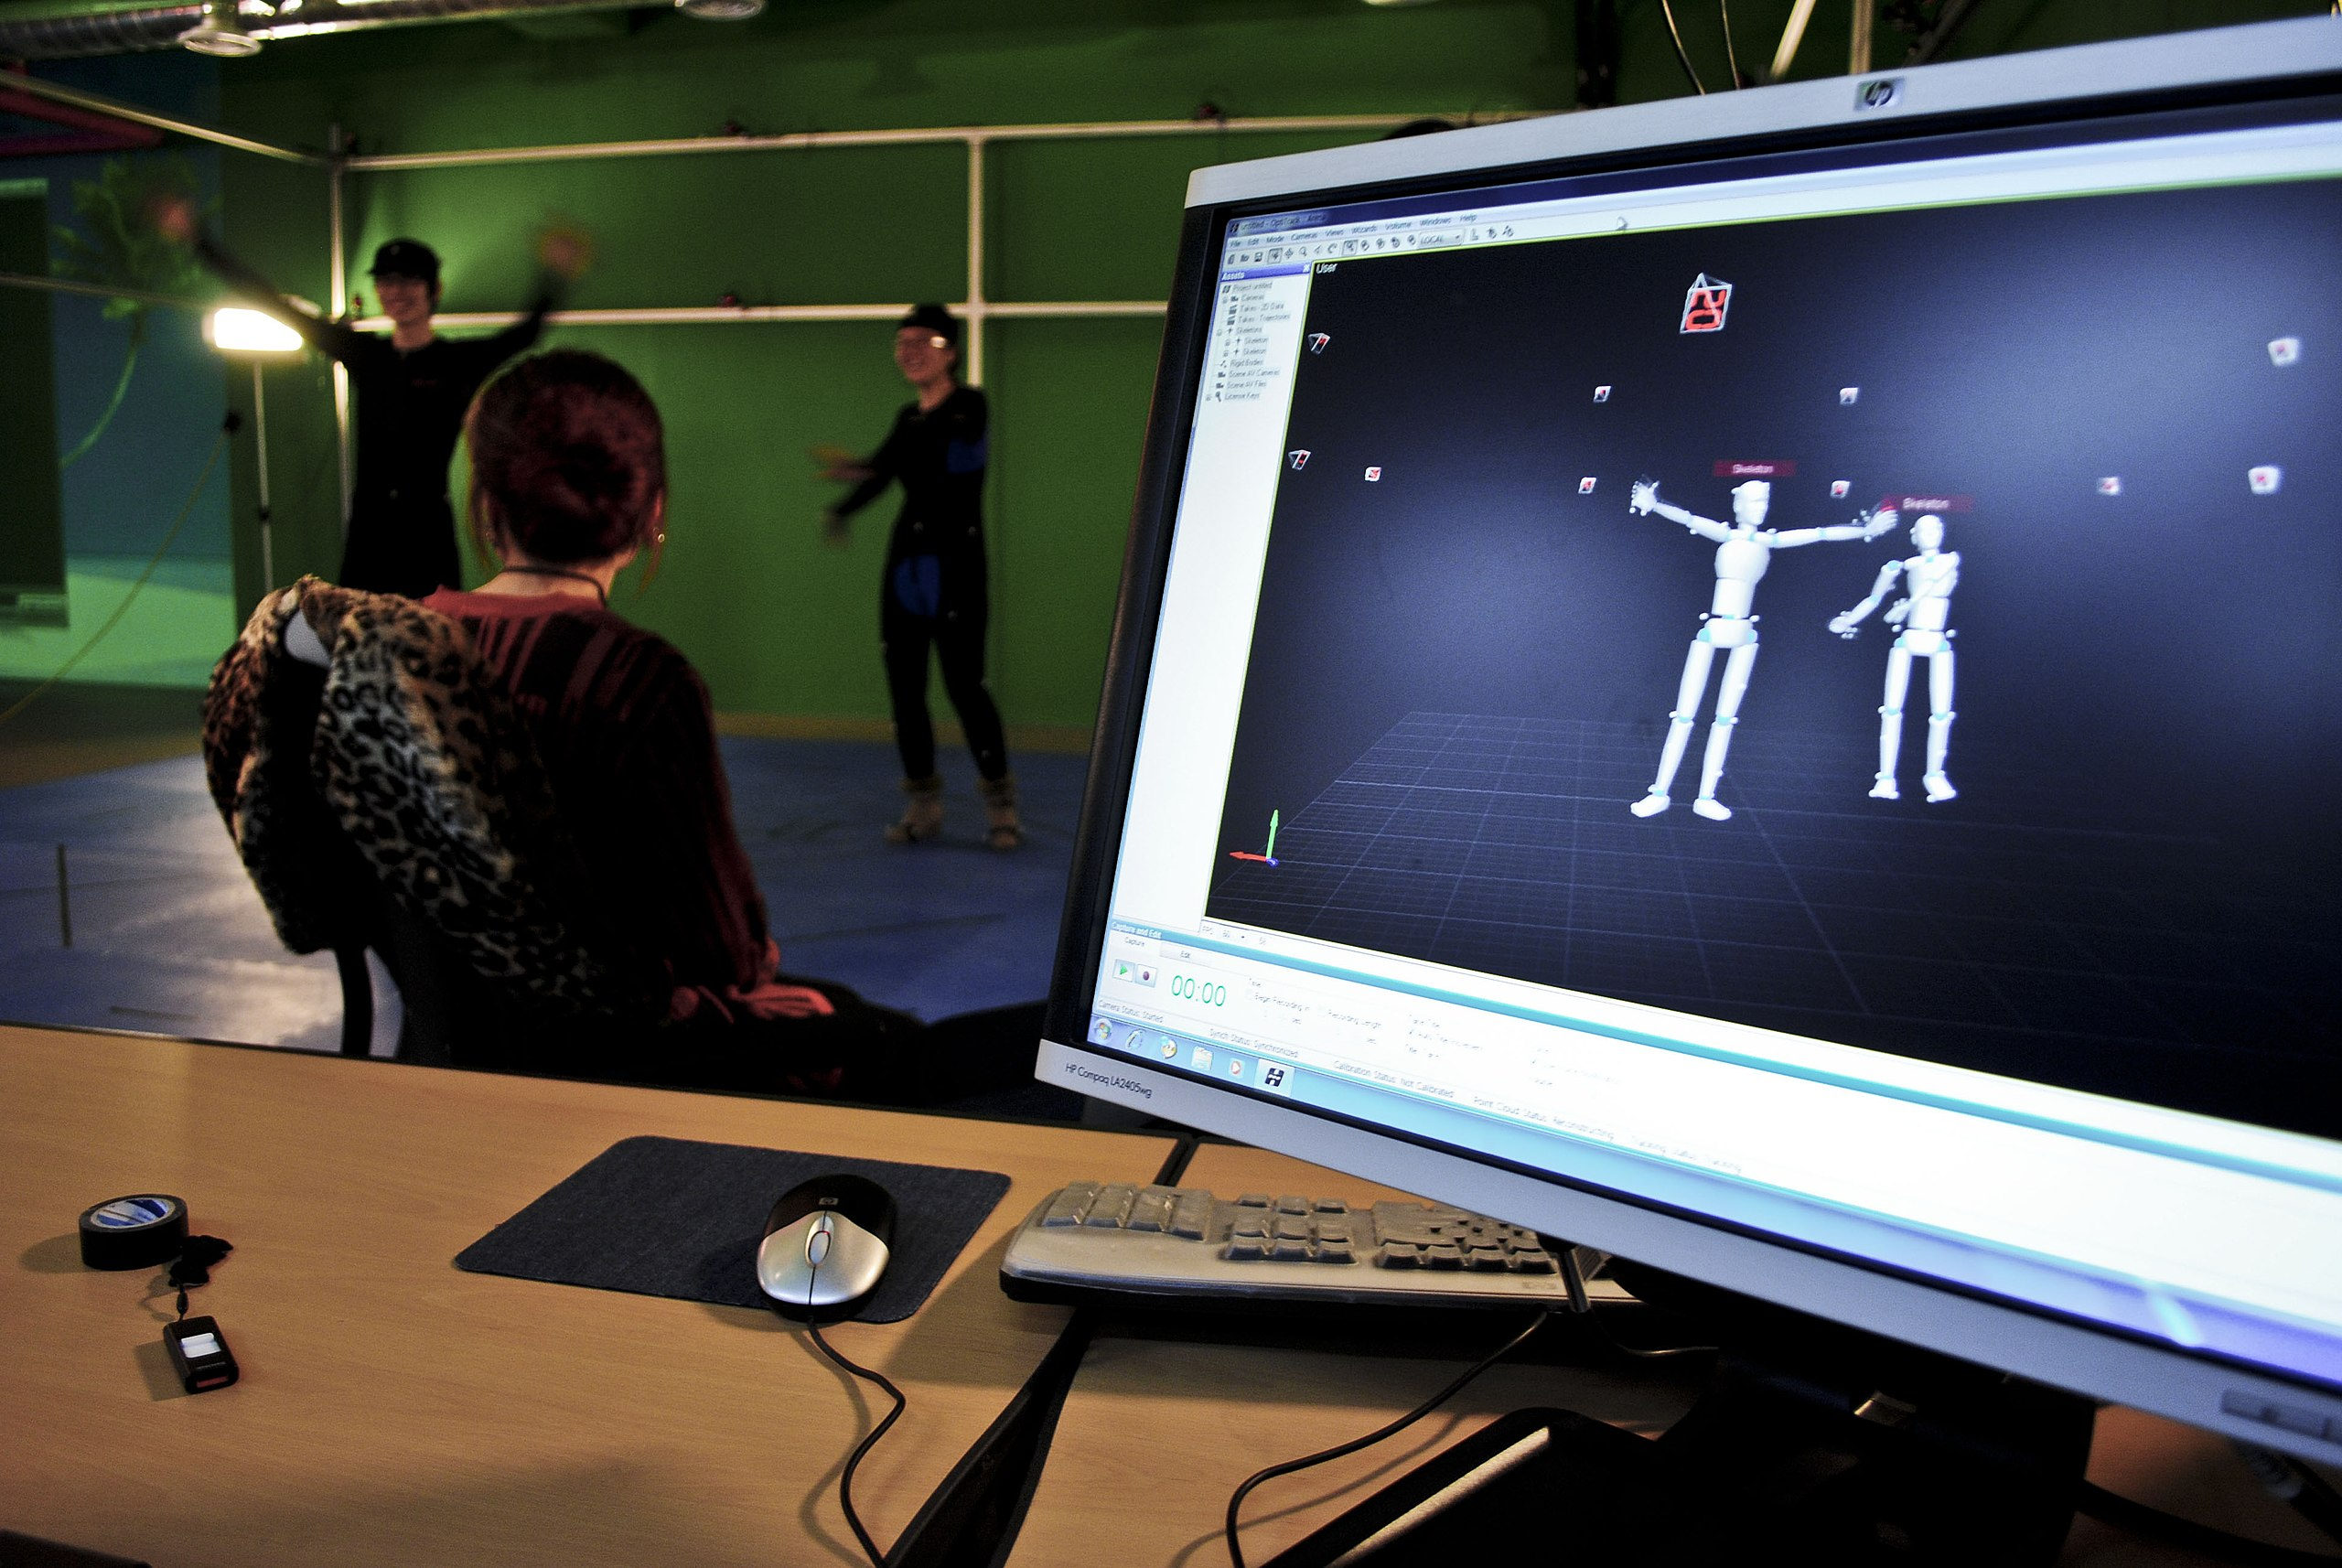
\includegraphics[width = 2.5in]{chapters/background_work/images/mocap.png} 
  \caption{Mocap capture and retargeting} 
  \label{fig:mocap} 
\end{figure}

Motion capture (mocap) retargeting offers a significant boost in animation speed and realism, but it does come with its challenges. It requires specialized equipment and involves intricate data processing, particularly when filtering out noise. Additionally, reusing mocap data across different avatars can be complex due to variations in body proportions and joint placements. Furthermore, segmenting mocap data into different parts for reuse can be difficult, limiting its flexibility in animation projects.

\paragraph{Kinematics}
\label{ch:background_work:sign_language_synthesis:3d_techniques:avatar_animation:kinematics}

Kinematics is used to define the motion of joints in a skeleton, allowing animators to create realistic and dynamic movements. Two key kinematic techniques used in avatar animation are \gls{fk} and \gls{ik}.

\subparagraph{\gls{fk}}
\label{ch:background_work:sign_language_synthesis:3d_techniques:avatar_animation:kinematics:forward_kinematics}

\gls{fk} is a method where the position and rotation of each joint in a skeleton are specified explicitly by the animator. This means that to move a hand, for example, the animator must adjust the shoulder, elbow, and wrist joints individually. \gls{fk} provides precise control over each joint, making it ideal for detailed and deliberate animations. However, it can be cumbersome for complex movements, as changes to one joint may require adjustments to multiple other joints to achieve a natural pose. Figure~\ref{fig:forward_kinematics_example} illustrates the forward kinematics process.

\begin{figure} 
  \centering 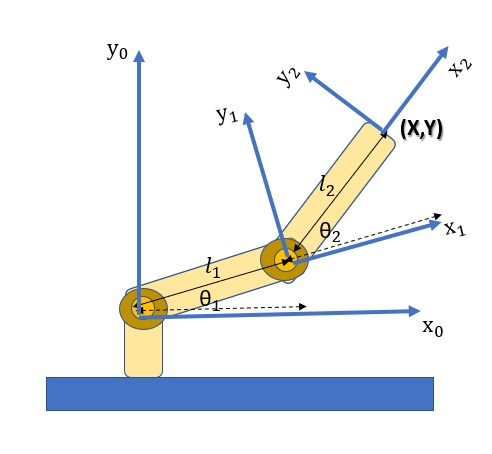
\includegraphics[width = 2.5in]{chapters/background_work/images/forward_kinematics_example.png} 
  \caption{FK} 
  \label{fig:forward_kinematics_example} 
\end{figure}

\subparagraph{\gls{ik}}
\label{ch:background_work:sign_language_synthesis:3d_techniques:avatar_animation:kinematics:inverse_kinematics}

\gls{ik} simplifies the animation process by allowing the animator to position the end effector (e.g., a palm or foot) directly (figure~\ref{fig:inverse_kinematics_example}). An \gls{ik} solver then computes the necessary joint rotations to achieve a desired position of the end effector. This technique is particularly useful for tasks like making a character’s hand reach a specific point or ensuring that feet remain planted on the ground. \gls{ik} is widely used in character animation to create natural and realistic movements more efficiently than \gls{fk}. \gls{ik} is popular area of research and there have been several ways to solve \gls{ik} problems.

\begin{figure} 
  \centering 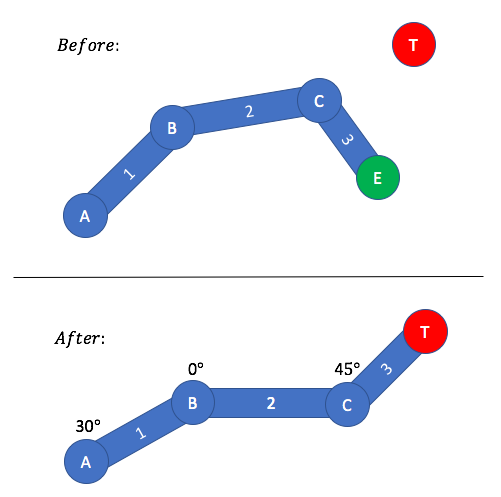
\includegraphics[width = 2.5in]{chapters/background_work/images/inverse_kinematics_example.png} 
  \caption{IK} 
  \label{fig:inverse_kinematics_example} 
\end{figure}

\begin{itemize} 
  \item \textbf{Jacobian-based methods}~\cite{4648032} solve the inverse kinematics (\gls{ik}) problem by linearizing the relationship between joint angles and end-effector positions through the calculation of the Jacobian matrix. These methods operate by formulating the \gls{ik} problem as a set of instantaneous task specifications, which are treated as constraints, such as positions, orientations, and other task-specific requirements. By iteratively adjusting joint angles to reduce the error between the current and target positions, they aim to minimize a cost function subject to multiple \gls{posture_constraint}s. Optimization techniques are employed to handle these constraints simultaneously, ensuring that the solution adheres to the defined task requirements. Despite their robustness in real-time applications, Jacobian-based methods can suffer from singularities, where solutions become unstable or unrealistic, as illustrated in Figure~\ref{fig:jacobian_based}.

  \item \textbf{\gls{ccd}}~\cite{kenwright2012inverse} simplifies the inverse kinematics (\gls{ik}) problem by adjusting one joint at a time to minimize the distance between the end-effector and the target position. It works by iteratively optimizing the position of each joint in the kinematic chain, starting from the end-effector and proceeding through each joint in sequence. This adjustment is done in a cyclic manner, where each joint is modified to ensure that the end-effector gets closer to the target while not significantly disrupting the previous adjustments. \gls{ccd} is computationally efficient and easy to implement, which makes it particularly popular in game engines. However, its greedy approach can lead to suboptimal solutions in more constrained or biomechanically complex setups, as illustrated in Figure~\ref{fig:ccdik}.

  \item \textbf{\gls{fabrik}}~\cite{aristidou2011fabrik} solves the inverse kinematics (\gls{ik}) problem through a two-phase iterative process: forward reaching and backward reaching. In the forward reaching phase, the algorithm starts from the base of the kinematic chain and moves towards the end-effector, adjusting joint positions to align with the target while respecting joint constraints. In the backward reaching phase, the process is reversed, starting from the end-effector and refining joint positions back toward the base to ensure convergence towards the target. Unlike other methods that focus on joint angles, \gls{fabrik} adjusts joint positions directly in two passes—from the end-effector to the root and back to the end-effector. This iterative process continues until the end-effector reaches the desired target within an acceptable tolerance. Known for its stability and simplicity, \gls{fabrik} is particularly effective in scenarios requiring natural joint configurations, as shown in Figure~\ref{fig:fabrik}.
\end{itemize}

\begin{figure}
    \centering 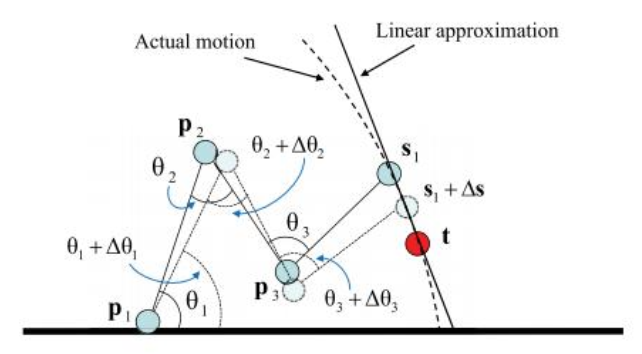
\includegraphics[width = 4in]{chapters/background_work/images/jacobian_based.png}
    \caption{Jacobian based IK solving (approximation of the first derivative)}
    \label{fig:jacobian_based}
\end{figure}

\begin{figure}
  \centering 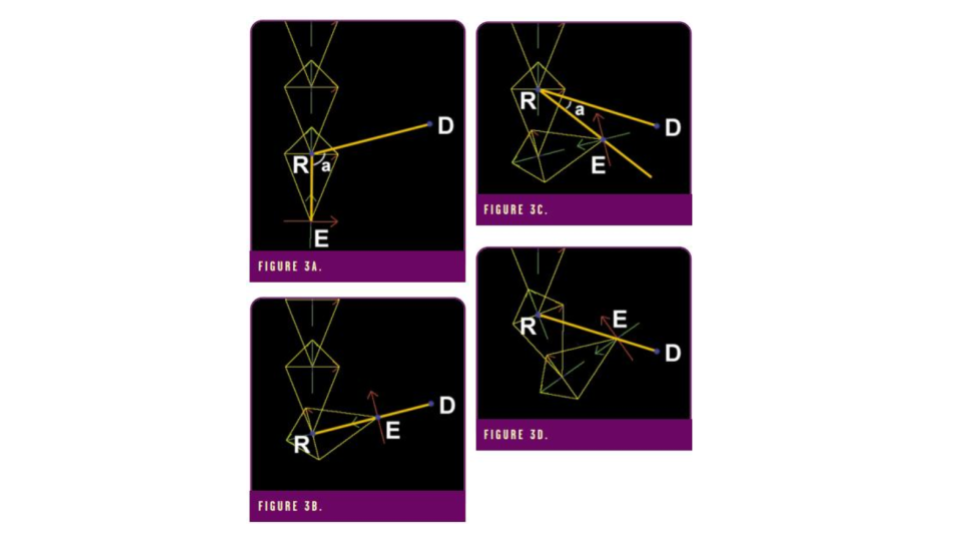
\includegraphics[width = 4in]{chapters/background_work/images/ccdik.png}
  \caption{Cyclic Coordinate Descent (CCD) IK solving (changes the rotation of a joint, one at a time)}
  \label{fig:ccdik}
\end{figure}

\begin{figure}
  \centering 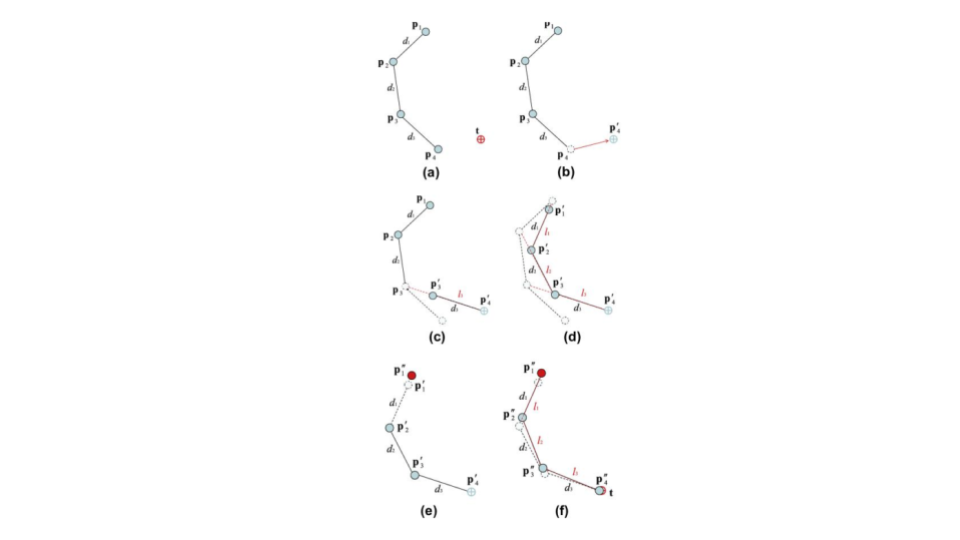
\includegraphics[width = 4in]{chapters/background_work/images/fabrik.png}
  \caption{FABRIK solving (updates coordinates in two passes)}
  \label{fig:fabrik}
\end{figure}

These classical \gls{ik} techniques, while computationally efficient, are prone to singularities, have limited support for complex joint constraints, and often result in unnatural or biomechanically unrealistic poses. As demonstrated in Figure~\ref{fig:problems_classical}, they struggle with overlapping chains and handling multiple end-effectors.

\begin{figure}
  \centering 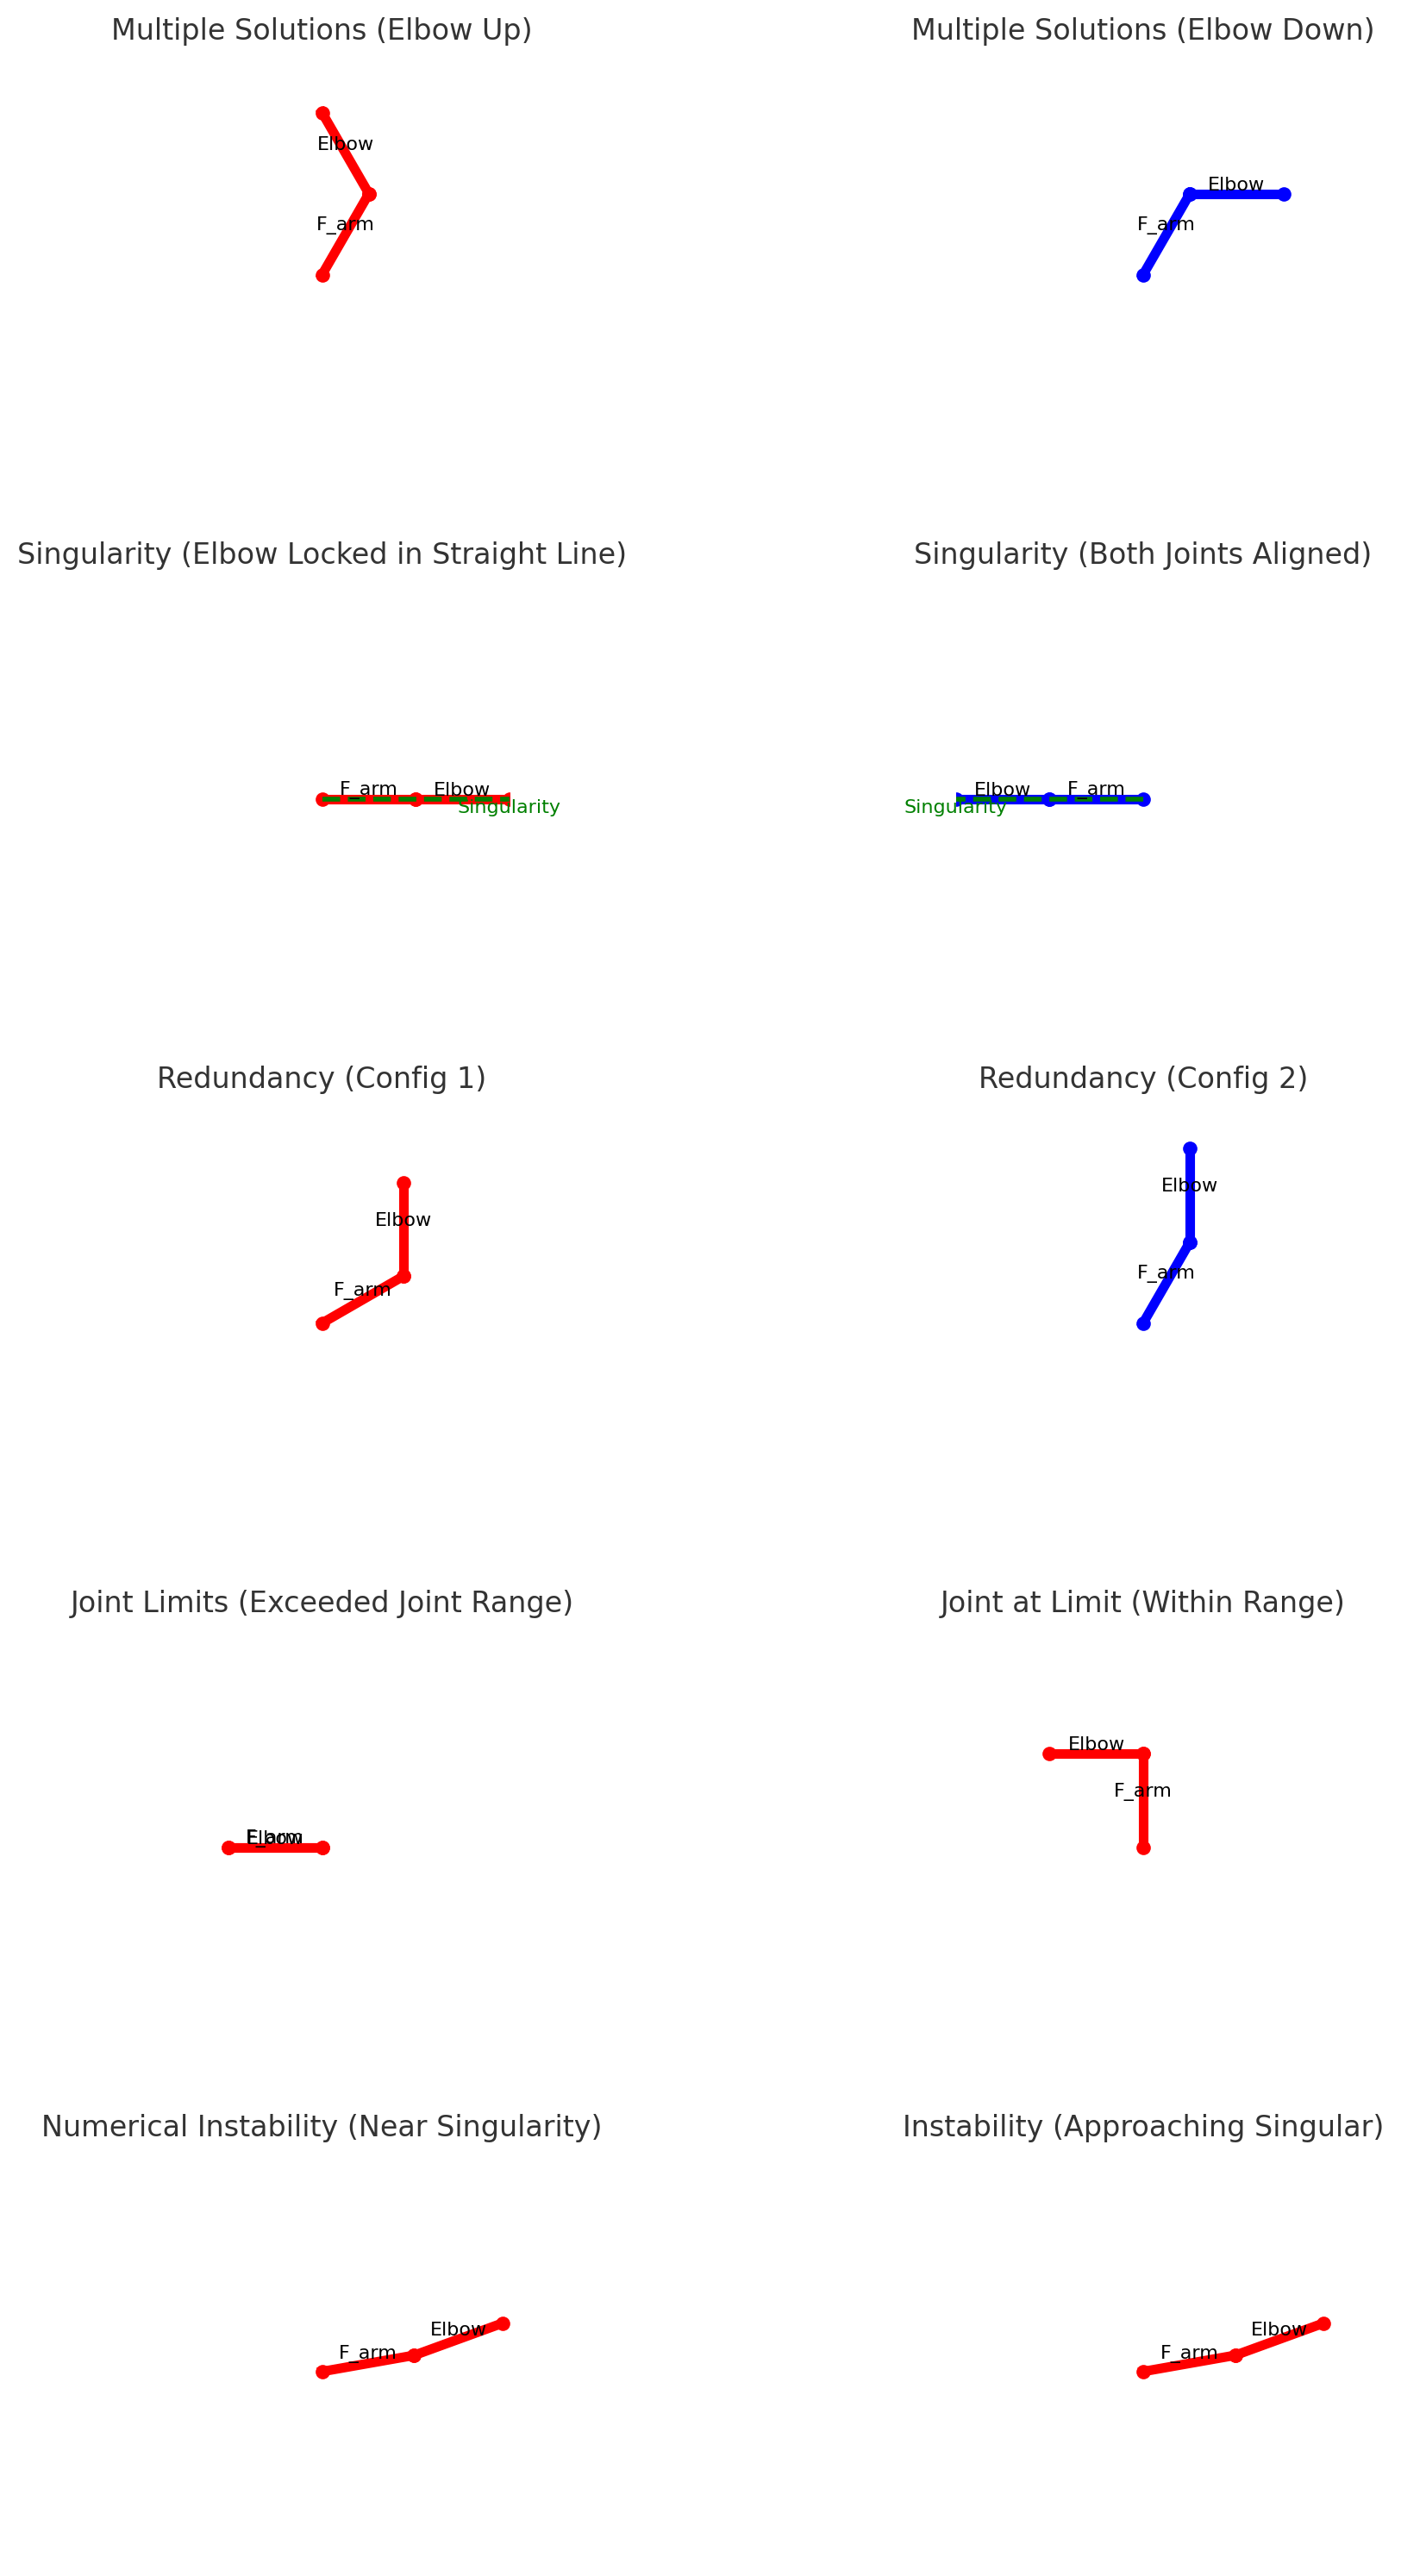
\includegraphics[width = 4in]{chapters/background_work/images/problems_classical.png}
  \caption{Problems with classical IK methods}
  \label{fig:problems_classical}
\end{figure}

\paragraph{Deep Learning and Character Animation}
\label{ch:background_work:sign_language_synthesis:3d_techniques:avatar_animation:deep_learning}

To address the shortcomings of classical kinematics methods, data-driven approaches have emerged, leveraging large datasets and machine learning to produce more flexible and realistic animations. This section explores some deep learning techniques used in character animation.

\subparagraph{Style-Based IK}
\label{ch:background_work:sign_language_synthesis:3d_techniques:avatar_animation:deep_learning:style_ik}

Style \gls{ik}~\cite{grochow2004style} leverages machine learning to represent poses in a \gls{latent_space} using \gls{sgplvm}. By learning the distribution of poses, Style \gls{ik} generates stylized animations that adhere to aesthetic or functional constraints, making it especially useful in scenarios where mocap data is unavailable or infeasible. Figure~\ref{fig:style_ik} shows how poses are mapped in \gls{latent_space} for Style IK.

\begin{figure}
  \centering 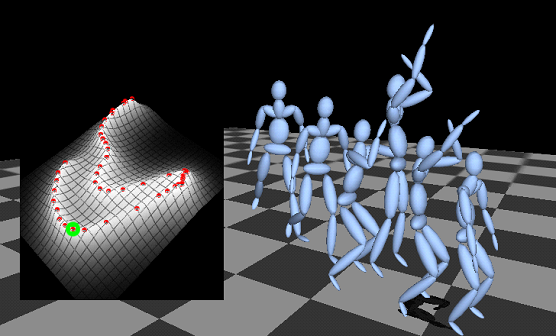
\includegraphics[width = 3in]{chapters/background_work/images/style_ik.png}
  \caption{Pose in latent space using Style IK}
  \label{fig:style_ik}
\end{figure}

\subparagraph{Motion Matching}
\label{ch:background_work:sign_language_synthesis:3d_techniques:avatar_animation:deep_learning:motion_matching}

Motion Matching represents a significant shift from traditional techniques by dynamically selecting the most appropriate animation from a large database of motion capture (mocap) data based on user inputs and contextual parameters. Ubisoft's \emph{For Honor} utilized this technique to create more fluid and responsive character animations, as shown in Figure~\ref{fig:for_honor}. Motion Matching's ability to break down animations into fine-grained clips allows for seamless transitions and natural movements.

\begin{figure}
  \centering 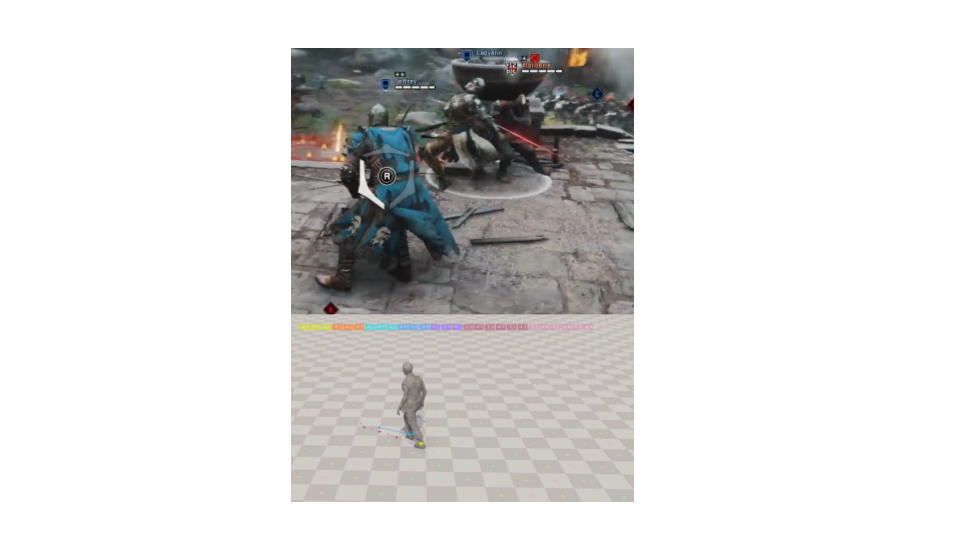
\includegraphics[width = 4in]{chapters/background_work/images/for_honor.png}
  \caption{Motion Matching in Ubisoft’s \emph{For Honor}}
  \label{fig:for_honor}
\end{figure}

\subparagraph{{PFNN}}
\label{ch:background_work:sign_language_synthesis:3d_techniques:avatar_animation:deep_learning:pfnn}

\gls{pfnn}~\cite{10.1145/3072959.3073663} extends the principles of motion matching by incorporating phase information into the neural network’s weights, allowing the network to generate animations that align with the cyclical nature of bipedal movement (walking, running). Unlike traditional methods that blend animation clips, PFNN encodes the entire animation process within the neural network, providing more control and flexibility, as illustrated in Figure~\ref{fig:pfnn}.

\begin{figure}
  \centering 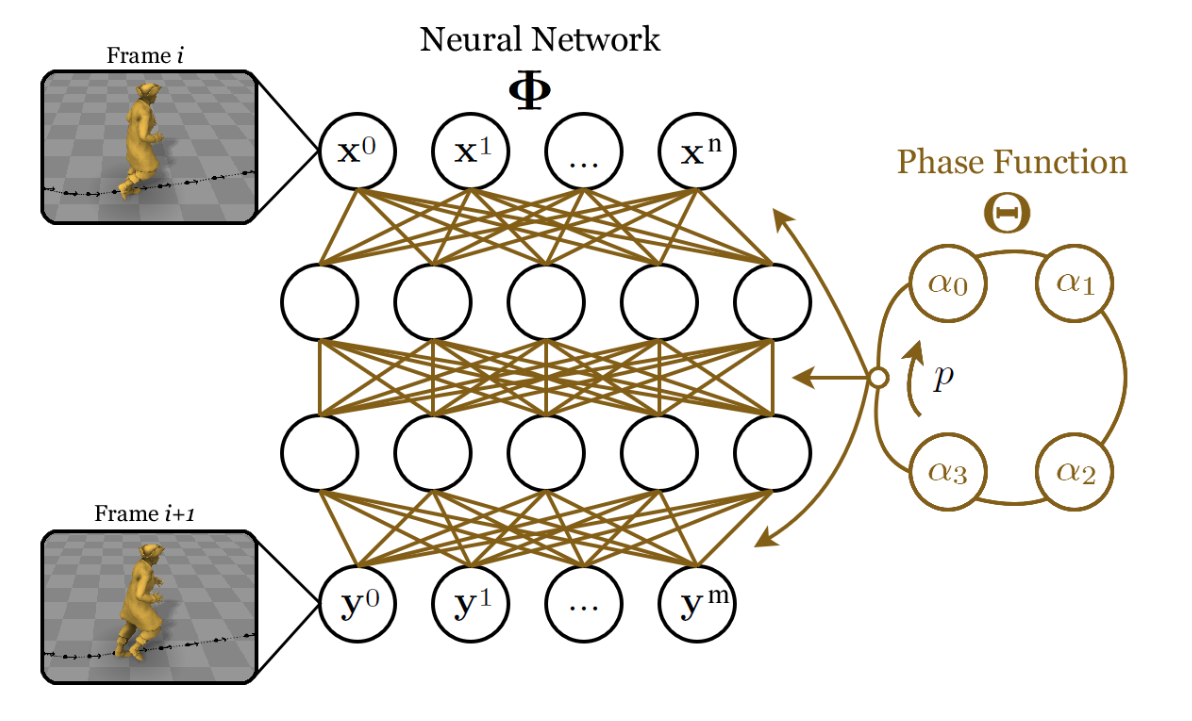
\includegraphics[width = 3in]{chapters/background_work/images/pfnn.png}
  \caption{Phase-Functioned Neural Networks (PFNN) for motion matching}
  \label{fig:pfnn}
\end{figure}

While these data-driven methods resolve many issues inherent to classical animation techniques, they bring challenges like the need for large amounts of training data and increased computational demands, particularly in real-time applications.

\subparagraph{Latent Space Representations for Pose Generation}
\label{ch:background_work:sign_language_synthesis:3d_techniques:avatar_animation:deep_learning:latent_space}

Latent space representations have become crucial in reducing the complexity of pose and motion data, allowing for more efficient and realistic pose generation and manipulation. \gls{vae}s~\cite{kingma2013auto}, such as those used in SMPLify-X~\cite{pavlakos2019expressive}, learn a probabilistic model of human poses. They can generate and manipulate poses in a lower-dimensional latent space, which can then be sampled to meet specific \gls{posture_constraint}s. SMPLify-X is particularly effective in estimating 3D poses from 2D images, as illustrated in Figure~\ref{fig:simplifyx}.

\begin{figure}
  \centering 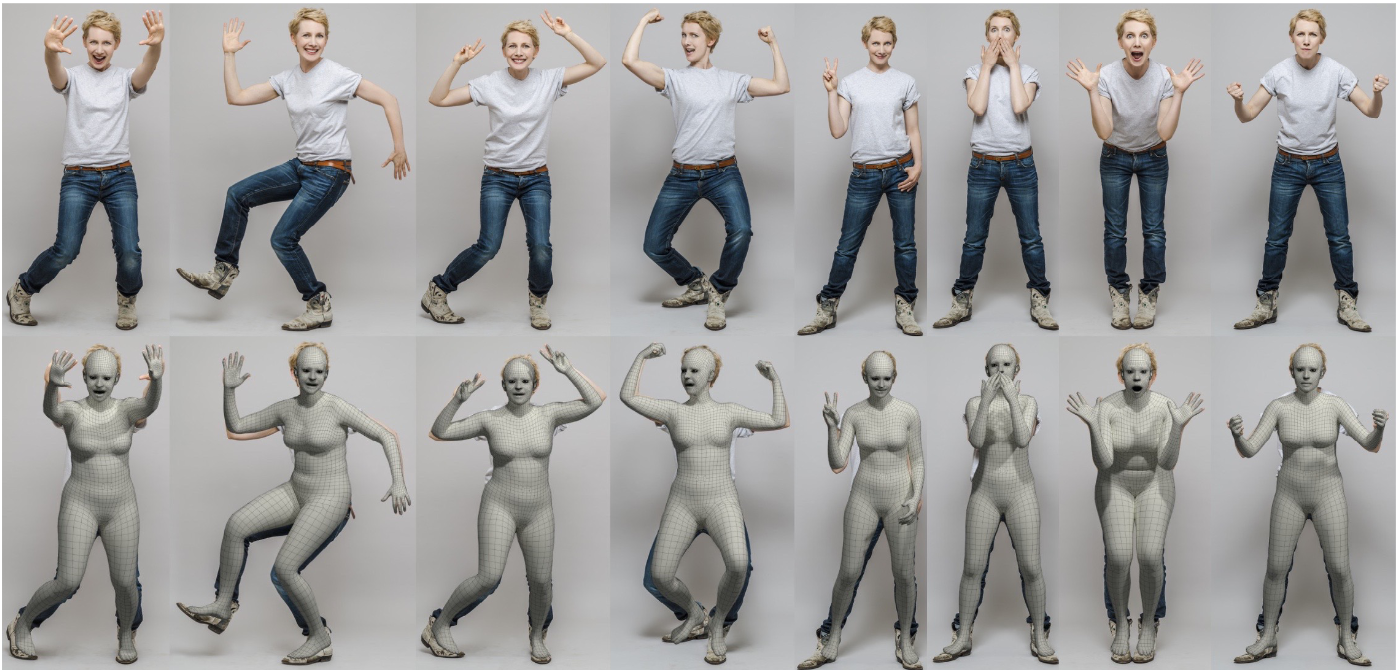
\includegraphics[width = 4in]{chapters/background_work/images/simplifyx.png}
  \caption{SMPLify-X generating poses from latent space}
  \label{fig:simplifyx}
\end{figure}

Pose manifolds~\cite{pavlakos2019expressive,tiwari2022pose, lu2023dposer} are pretty successful in creating a \gls{latent_space} representation of human poses. These manifolds are used to generate realistic and contextually appropriate poses by sampling from the learned distribution (a prior of human poses). This approach is particularly useful in generating diverse and expressive animations that adhere to specific constraints, such as bio-mechanical realism or stylistic preferences. Such pose manifolds can play a critical role by constraining pose generation to physically plausible configurations, as seen in figure~\ref{fig:pose_manifolds}.

\begin{figure}
  \centering 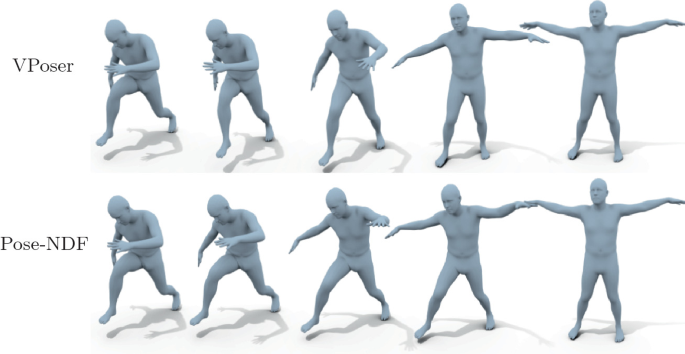
\includegraphics[width = 4in]{chapters/background_work/images/pose_manifolds.png}
  \caption{Pose regularization in a latent space}
  \label{fig:pose_manifolds}
\end{figure}

\paragraph{Representing Animation}
\label{ch:background_work:sign_language_synthesis:3d_techniques:avatar_animation:animation_timeline}

Animation timelines are often represented in the form of an animation timeline which provides visual representation of keyframes, motion curves, and other animation data. Animators use the timeline to organize and sequence animations, adjust timing and spacing, and fine-tune the overall motion of the avatar. Figure~\ref{fig:animation_timeline} shows an example of an animation timeline in Blender, a popular 3D animation software.

\begin{figure} 
  \centering 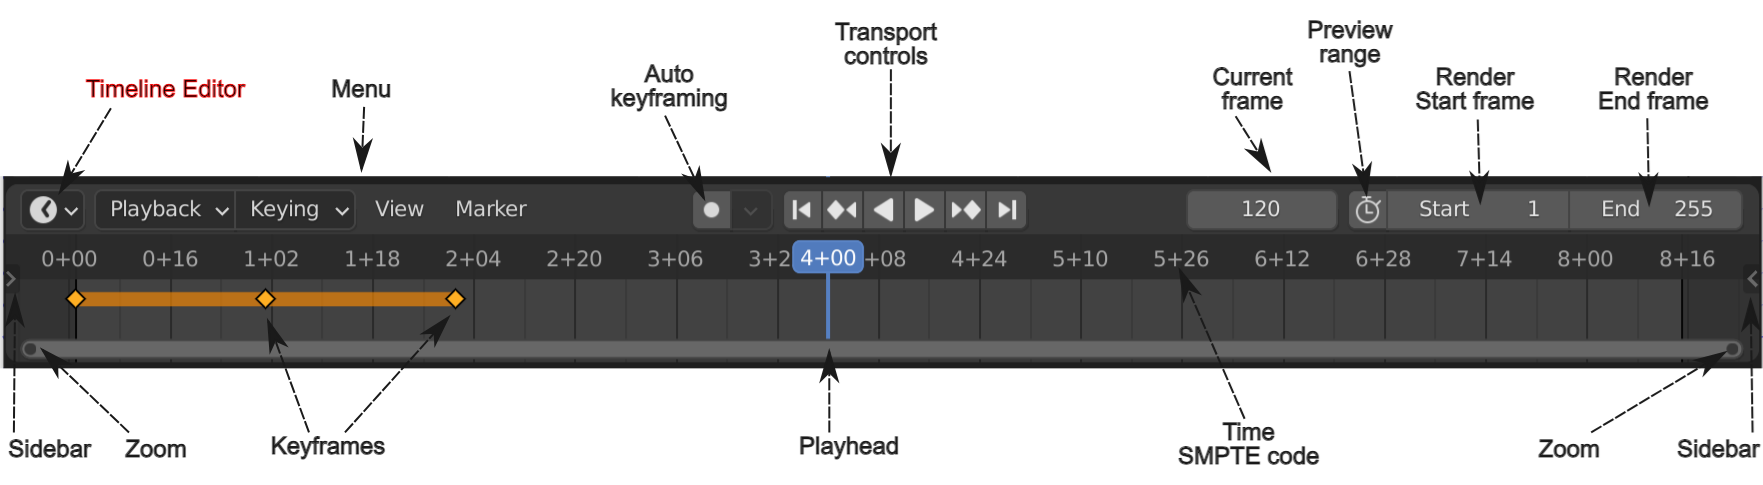
\includegraphics[width = 4in]{chapters/background_work/images/animation_timeline.png}
  \caption{Animation timeline in Blender} 
  \label{fig:animation_timeline}
\end{figure}

A multi-track timeline is a more advanced version of the animation timeline that allows animators to work with multiple tracks simultaneously. Multi-track interfaces are commonly used in video editing (figure~\ref{fig:video_edit}) and animation software to manage complex animations with multiple layers of motion data. Figure~\ref{fig:nle_editor} illustrates the \gls{nle} interface in blender, which represent the animation timeline in a multi-track format.

\begin{figure}
    \centering
    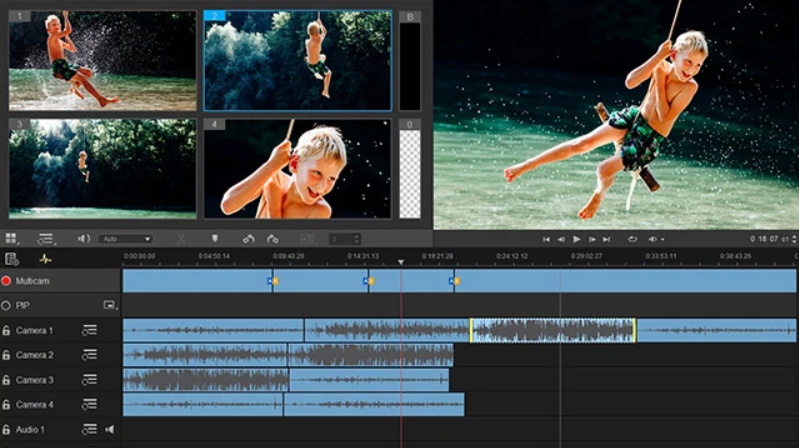
\includegraphics[width=0.8\textwidth]{chapters/background_work/images/video_editing.png}
    \caption{Video editing software interfaces with multiple tracks for editing video and audio clips.}
    \label{fig:video_edit}
\end{figure}

\begin{figure}
    \centering
    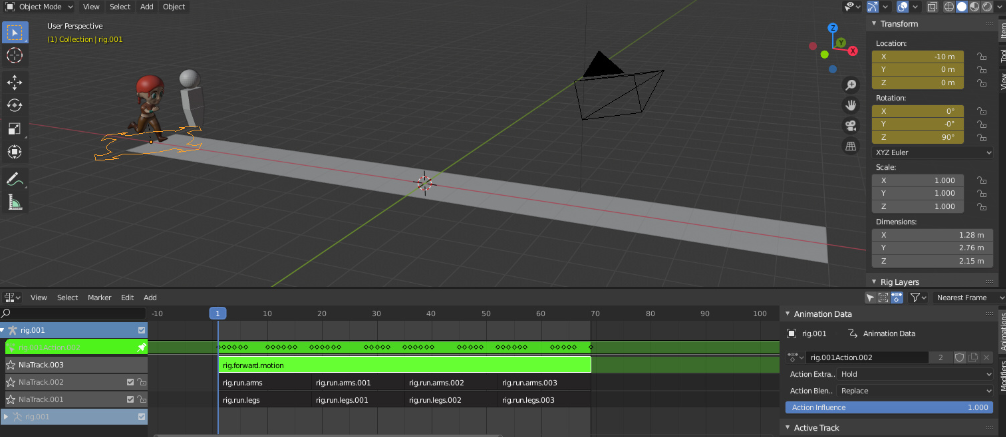
\includegraphics[width=0.8\textwidth]{chapters/background_work/images/nle_blender.png}
    \caption{Blender's NLE showing multiple tracks for editing animation clips.}
    \label{fig:nle_editor}
\end{figure}

Apart from artists, researchers too have recently explored multi-track timeline control for text-driven 3D human motion generation~\cite{petrovich24stmc}. The work introduces a novel way to address the limitations of previous methods that lacked fine-grained control over action composition and timing. This approach allows users to define multiple textual prompts within overlapping temporal intervals, enabling precise control over complex actions (figure~\ref{fig:multi_track_other}). The proposed Spatio-Temporal Motion Collage (STMC) method, which operates at test-time, integrates with pre-trained motion diffusion models to generate realistic motions that adhere to the specified timeline. However, it is not for use in \gls{sl} synthesis, where precise and context-sensitive hand and body gestures are required, as it relies heavily on models not specifically designed for such detailed tasks.

\begin{figure}
    \centering
    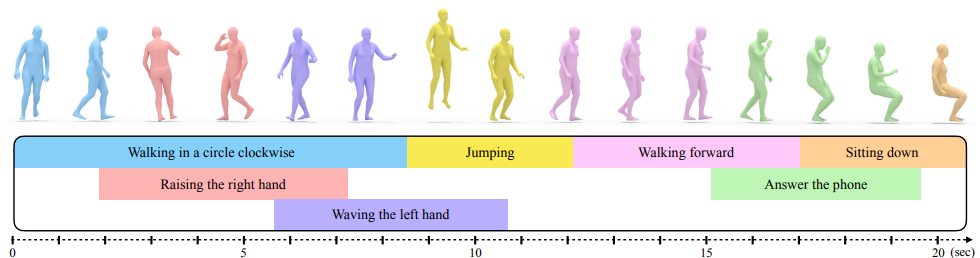
\includegraphics[width=0.9\textwidth]{chapters/background_work/images/multi_track_other.png}
    \caption{Multi-track timeline control for text-driven 3D human motion generation.}
    \label{fig:multi_track_other}
\end{figure}

In the context of \gls{sl} synthesis, a multi-track timeline is used by Paula~\cite{filhol2017synthesizing} (more discussed in section~\ref{ch:background_work:sign_language_synthesis:3d_techniques:sign_language_synthesis_systems:azee_based:paula}), a system that uses pre-animated motion data to generate multi-track animations using AZee. Paula's interface is tailored for creating \gls{sl} content, with each track representing a different aspect of the \gls{sl}. Figure~\ref{fig:paula} shows the Paula interface with a multi-track timeline for \gls{sl} synthesis.

\begin{figure}[h]
    \centering
    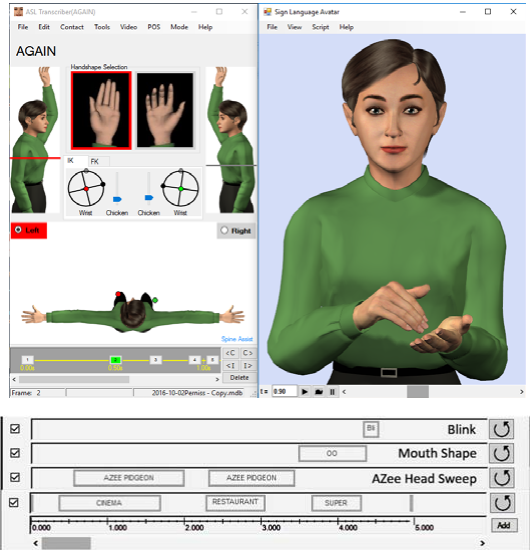
\includegraphics[width=0.8\textwidth]{chapters/background_work/images/paula_multi_track.png}
    \caption{Paula interface showing a multi-track timeline for SL synthesis.}
    \label{fig:paula}
\end{figure}

\paragraph{Motion Curves}
\label{ch:background_work:sign_language_synthesis:3d_techniques:avatar_animation:motion_curves}

Motion curves, have been extensively used in 3D character animation to control the timing and spacing of movements. These curves provide a graphical representation of a parameter's change over time, making them an essential tool in achieving realistic and fluid motion in animations(figure~\ref{fig:fcurves_blender}). Early foundational work by Witkin and Kass~\cite{witkin1988spacetime} introduced spacetime constraints, which used optimization techniques to control motion curves in generating realistic animations under physical constraints. This idea has evolved, and modern techniques now integrate deep learning models with motion curves to enhance control and automate the generation of complex animations. This is particularly useful in applications like motion inbetweening, where interpolating between keyframes requires precise control over motion curves to ensure smooth transitions and realistic movements (figure~\ref{fig:inbetweening_transformers})~\cite{10.1145/3550454.3555454}. However, traditional mathematical optimization techniques are still widely in use. For example use of tangent-space optimization~~\cite{10.1145/3306346.3322938} to control character interpolations by allowing animators to directly manipulate positions and orientations of the posture by manipulating the tangent of the curve. This minimizes the need for additional keyframes. It also ensures smooth transitions while respecting \gls{posture_constraint}s like joint limits and contact points, integrating seamlessly into existing animation workflows (figure~\ref{fig:inbetweening_disney}). 

\begin{figure}
    \centering 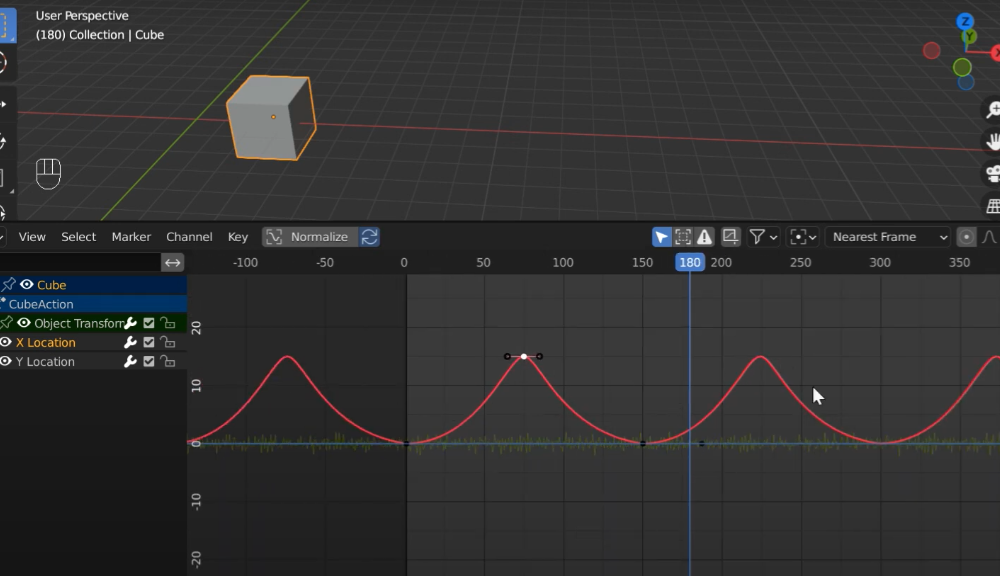
\includegraphics[width = 2.5in]{chapters/background_work/images/fcurves_blender.png}
    \caption{F-curves in Blender}
    \label{fig:fcurves_blender}
\end{figure}

\begin{figure}
    \centering 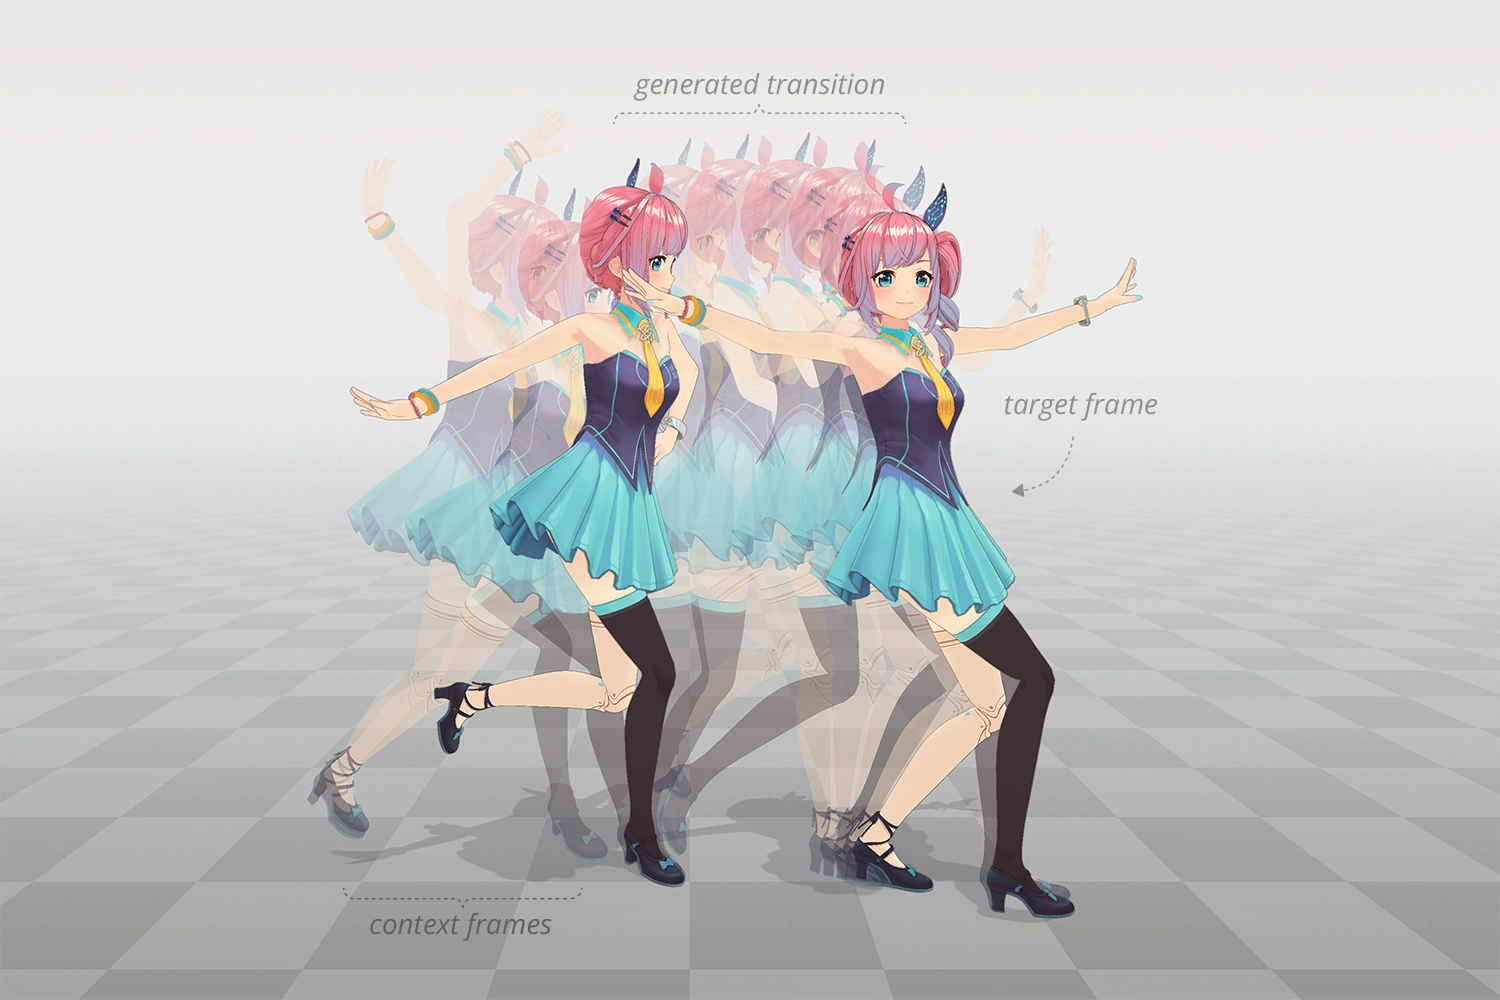
\includegraphics[width = 2.5in]{chapters/background_work/images/inbetweening_transformers.jpg}
    \caption{Motion Inbetweening using 2 stage Transformers~\cite{10.1145/3306346.3322938}}
    \label{fig:inbetweening_transformers}
\end{figure}

\begin{figure}
    \centering 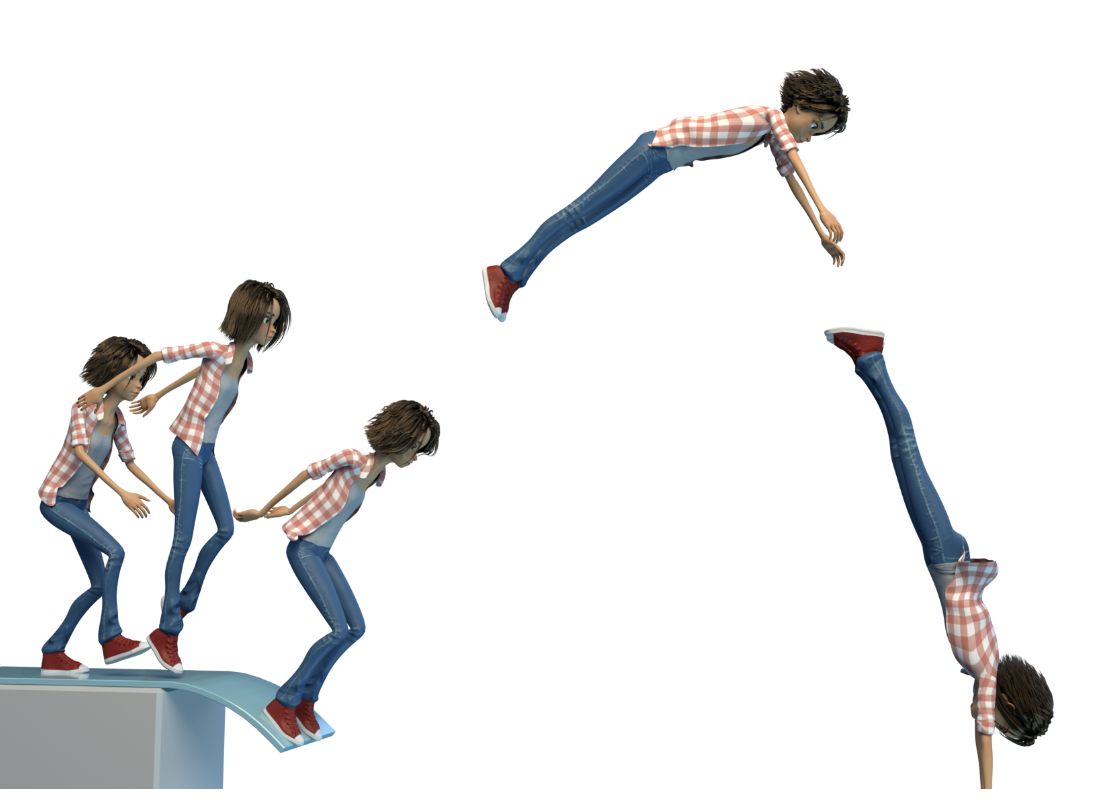
\includegraphics[width = 2.5in]{chapters/background_work/images/inbetweening_disney.png}
    \caption{Tangent-Space Optimization used to create dive animation}
    \label{fig:inbetweening_disney}
\end{figure}

In the context of \gls{sl} synthesis, SIGN MOTION~\cite{inproceedings} discuss the use of 3D motion analysis to accurately capture and animate \gls{sl} gestures by extracting motion curve parameters from sensors like Microsoft Kinect. These motion curves, which represent the trajectories of movements made during signing, are essential for animating virtual signers in a natural and precise manner. The paper highlights how these curves are mathematically defined, including their type, plane of motion, and velocity, which are then used to recreate realistic \gls{sl} animations, enhancing applications like \gls{sl} recognition and machine translation.

\paragraph{Motion Templates}
\label{ch:background_work:sign_language_synthesis:3d_techniques:avatar_animation:motion_templates}

Motion templates offer a reusable framework for applying pre-defined motion patterns across different characters or scenarios. These templates are essentially built upon motion curves that define the motion's parameters, allowing for efficient replication and adaptation of complex motions. The concept of motion templates has been widely adopted in various fields, from character animation to robotic motion planning. Modern approaches often combine motion templates with machine learning techniques to facilitate the adaptation of these templates to new contexts, such as different character anatomies or environmental conditions.

In the context of character animation, motion templates can be particularly advantageous. The reusable nature of these templates allows for the consistent production of motion across different avatars while ensuring that the nuances of each motion are preserved. A method for controlling avatars using clustered motion segments from a large motion capture database was introduced by~\cite{10.1145/566654.566607}, enabling efficient real-time animation with an intuitive user interfaces.

\paragraph{Procedural Animation}
\label{ch:background_work:sign_language_synthesis:3d_techniques:avatar_animation:procedural_animation}

Procedural animation techniques use algorithms and rules to generate motion automatically, rather than relying on manual keyframing or motion capture data. These techniques are particularly useful for creating dynamic and responsive animations that adapt to changing conditions or user interactions. Procedural animation can be applied to various aspects of avatar animation, including locomotion, facial expressions, and secondary motion.

\subparagraph{Data-Driven Constraint-Based Motion Editing}
\label{ch:background_work:sign_language_synthesis:3d_techniques:avatar_animation:procedural_techniques:data_driven_constraint_based_motion_editing}

Data-driven constraint-based motion editing~\cite{inbook} combines model-based and goal-directed techniques to enhance human motion animation. The system incorporates Prioritized \gls{ik} to solve for joint movements that meet user-defined constraints. Animators can use key-frame and key-trajectory \gls{posture_constraint}s to specify end-effector positions and paths, simplifying the animation process. The optimization step ensures smooth, continuous motions, avoiding common artifacts and preserving the natural flow of movement.

\subparagraph{Deep Learning based Techniques}
\label{ch:background_work:sign_language_synthesis:3d_techniques:avatar_animation:procedural_techniques:deep_learning_based_techniques}

Deep learning-based techniques have shown significant promise in procedural animation, particularly in the generation of realistic and dynamic movements. Neural networks can be trained on large datasets of motion data to learn complex patterns and generate new animations. For example, diffusion models have been used to synthesize human-like motion sequences with high fidelity and diversity from text prompts. Treating character animation as a cross-modal translation task where descriptive sentences serve as inputs to generate corresponding avatar animations. These techniques, however, require large amounts of data and computational resources to train effectively. Figure~\ref{fig:deep_learning_synthesis} shows an example of deep learning-based synthesis.

\begin{figure} 
  \centering 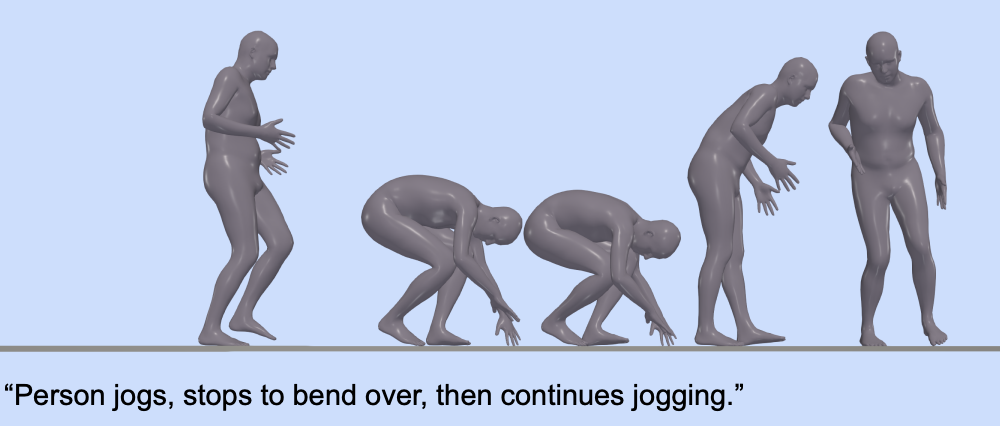
\includegraphics[width = 4in]{chapters/background_work/images/deep_learning_synthesis.png} 
  \caption{Deep Learning based synthesis} 
  \label{fig:deep_learning_synthesis} 
\end{figure}

\subparagraph{Hybrid Workflows}
\label{ch:background_work:sign_language_synthesis:3d_techniques:avatar_animation:procedural_techniques:hybrid_workflows}

Hybrid worflows combine elements of manual keyframing, mocap retargeting, and procedural techniques to leverage the strengths of each method. By integrating these approaches, animators can achieve a balance between control, efficiency, and realism. For instance, an animator might use mocap data as a base and then refine specific movements with manual keyframes to enhance expressiveness. Additionally, procedural techniques can be applied to automate repetitive tasks or to ensure that certain \gls{posture_constraint}s are met dynamically during the animation process. Hybrid workflows offer a flexible and powerful workflow, allowing for the creation of complex animations that are both realistic and tailored to the specific needs of a project. Figure~\ref{fig:cascadeur} shows an example of a hybrid animation tool, Cascadeur.

\begin{figure} 
  \centering 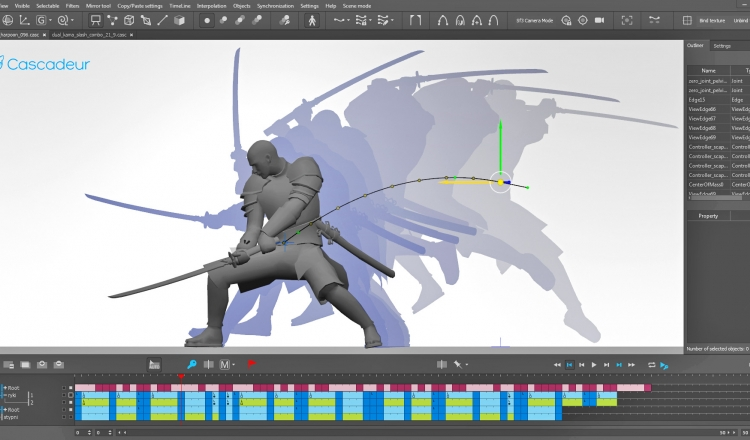
\includegraphics[width = 4in]{chapters/background_work/images/cascadeur.png} 
  \caption{Cascadeur hybrid animation tool} 
  \label{fig:cascadeur} 
\end{figure}

\paragraph{Face Animation}
\label{ch:background_work:sign_language_synthesis:3d_techniques:avatar_animation:face_animation}

This section explores rigging as well as animation of an avatar's face.

\subparagraph{Face Rigging}
\label{ch:background_work:sign_language_synthesis:3d_techniques:avatar_animation:face_animation:face_rigging}

Face rigging is the process of creating a digital framework that allows for the animation of facial expressions. There are several approaches to face rigging, each with its own advantages and disadvantages.

Blendshape-based rigging involves creating a set of predefined facial shapes (blendshapes) that represent various expressions (figure~\ref{fig:blendshapes_smile}). Multiple versions of a mesh are stored to achieve this and interpolating between these meshes allows animators to blend between various expressions smoothly, such as smiling, frowning, or blinking. These blendshapes can be blended together in different proportions to create a wide range of facial expressions. However, it requires a large number of blendshapes to capture all possible expressions.

\begin{figure}[h]
  \centering
  \begin{subfigure}{0.3\linewidth} 
      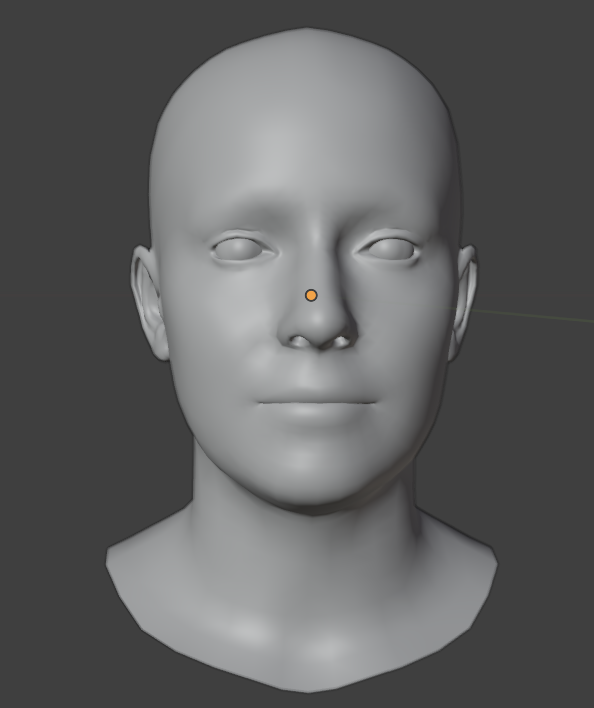
\includegraphics[width=\linewidth]{chapters/background_work/images/blendshapes_example/blendshapes_example_1.png} 
      \caption{Smile at 0} 
  \end{subfigure} 
  \hfill 
  \begin{subfigure}{0.3\linewidth} 
      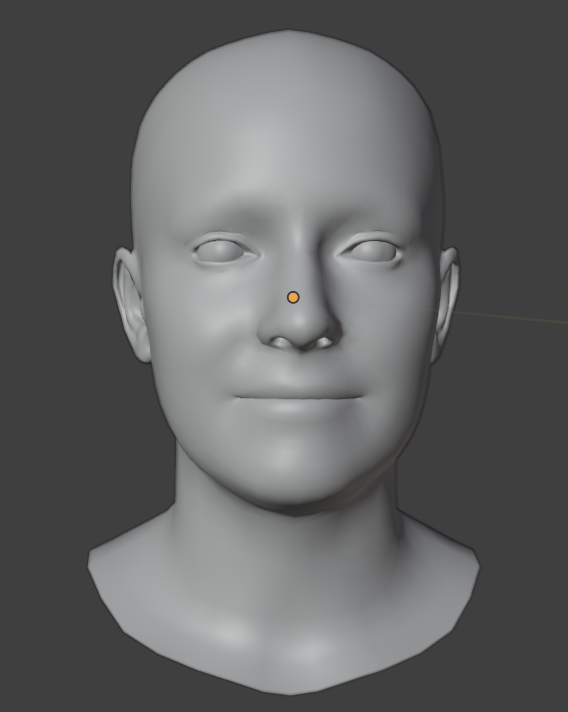
\includegraphics[width=\linewidth]{chapters/background_work/images/blendshapes_example/blendshapes_example_2.png} 
      \caption{Smile at 0.5} 
  \end{subfigure} 
  \hfill 
  \begin{subfigure}{0.3\linewidth} 
      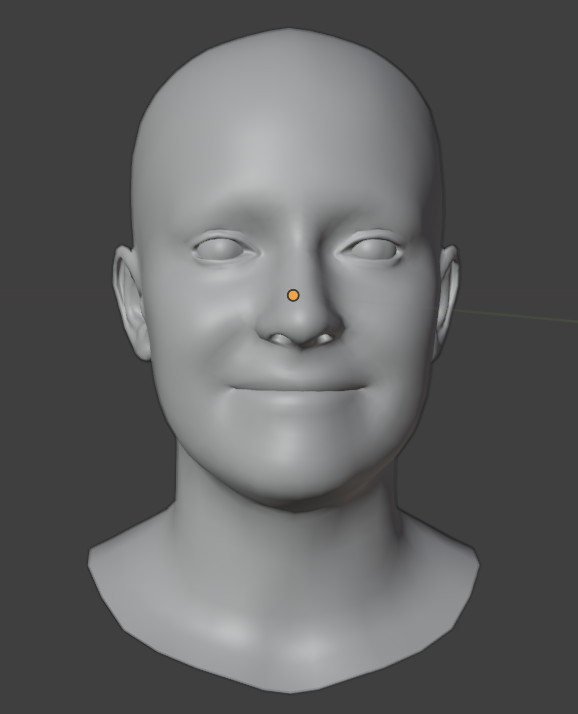
\includegraphics[width=\linewidth]{chapters/background_work/images/blendshapes_example/blendshapes_example_3.png} 
      \caption{Smile at 1} 
  \end{subfigure}
  \caption{Progression of smile using blendshapes from 0 to 1.0}
  \label{fig:blendshapes_smile}
\end{figure}

Skeleton-based rigging uses a hierarchical system of bones and joints to control facial movements (figure~\ref{ch:facial_expressions:fig:skeleton_based_rigging}). Each bone can control different parts of the face, such as the jaw, eyebrows, and eyelids. This offers more granular control but can be less intuitive than blendshapes for subtle expressions.

\begin{figure}
    \centering
    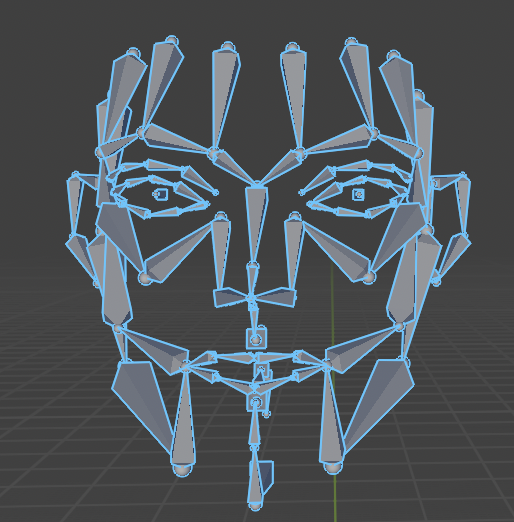
\includegraphics[width=0.8\textwidth]{chapters/background_work/images/facial_bones.png}
    \caption{Skeleton-based rigging for facial expressions}
    \label{ch:facial_expressions:fig:skeleton_based_rigging}
\end{figure}

The use of blendshape-based rigging or skeleton-based rigging depends on the goal. More generally: 

\begin{itemize}
  \item \textbf{blendshapes}: Ideal for detailed and smooth transitions between expressions, but limited in flexibility.
  \item \textbf{Bones}: Provide granular control, better for interactive or dynamic facial animations but are more complex to set up and manage.
\end{itemize}

Usually, the two techniques are combined to offer greater flexibility and control.

\subparagraph{Capturing Facial Expressions}
\label{ch:background_work:sign_language_synthesis:3d_techniques:avatar_animation:face_animation:capturing_facial_expressions}

Facial expressions can be captured manually or through performance-based techniques.

Manual keyframing is a foundational animation technique, where animators manually set key poses (figure~\ref{ch:facial_expressions:fig:keyframing}). It is effective but may struggle to capture the variability required in \gls{sl} synthesis.

\begin{figure}
    \centering
    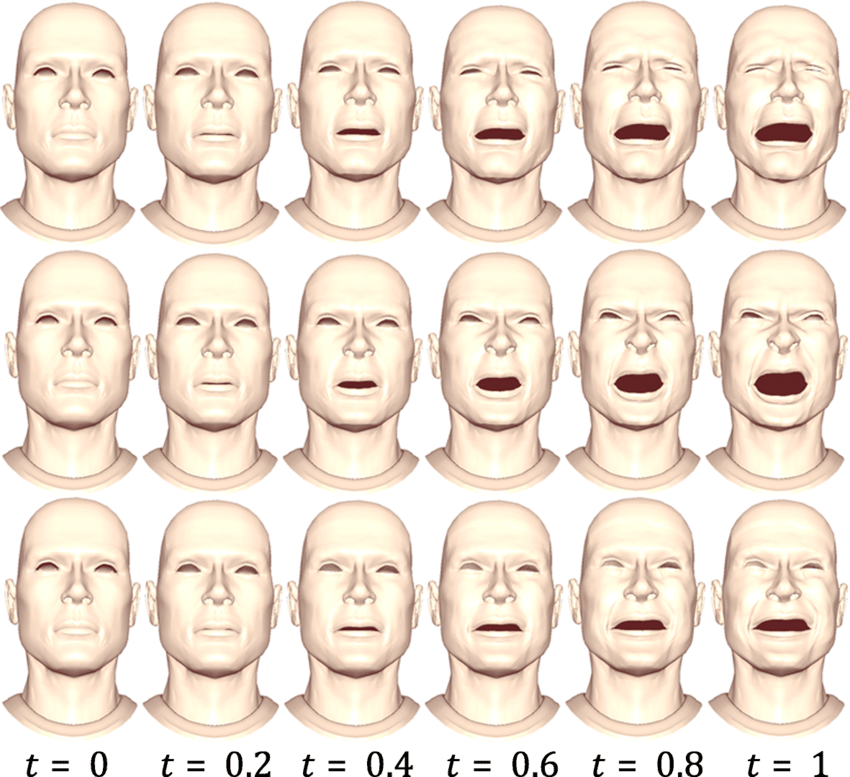
\includegraphics[width=0.8\textwidth]{chapters/background_work/images/facial_keyframing.png}
    \caption{Keyframing process, showing how key poses are set and interpolated to create a continuous animation.}
    \label{ch:facial_expressions:fig:keyframing}
\end{figure}

Performance-based motion capture captures human facial movements and uses this data to animate digital avatars. Tools like Apple's ARKit (figure~\ref{ch:facial_expressions:fig:motion_capture}) are examples of this approach.

\begin{figure}
    \centering
    \includegraphics[width=0.8\textwidth]{chapters/background_work/images/facial_motion_capture.jpg}
    \caption{Performance-based facial animation using Apple's ARKit}
    \label{ch:facial_expressions:fig:motion_capture}
\end{figure}

\subparagraph{Facial Expressions Synthesis}
\label{ch:background_work:sign_language_synthesis:3d_techniques:avatar_animation:face_animation:facial_expressions_synthesis}

Most facial expression research is motivated by synthesis from voice signals. These methods are generally categorized into lip-sync techniques~\cite{yousaidthat, talkingface, lipmovements, lipsyncexpert}, which align mouth movements with audio, and full-face expression synthesis~\cite{eskimez, greenwood18, controllable_facial_synth}. Some approaches model speaking style with 3D animation parameters~\cite{cudeiro}, or create generalized latent audio expressions combined with a person-specific 3D model~\cite{FLAME}. Related work, MakeItTalk~\cite{Yang:2020:MakeItTalk}, introduces a two-stage deep learning model that predicts facial landmark displacements based on audio input, followed by an image-to-image translation method to generate the final facial expression. 

\subparagraph{Emotion Recognition}
\label{ch:background_work:sign_language_synthesis:3d_techniques:avatar_animation:face_animation:emotion_recognition}

Emotion recognition systems use machine learning algorithms to analyze facial features and identify the underlying emotional state. The most common approach to define emotions is Ekman's \gls{facs}~\cite{ekman1978facial}, which categorizes facial expressions into action units (AUs) (figure~\ref{fig:action_units}). Various deep learning models have been developed to recognize AUs and emotions from facial images. One such model~\cite{luo2022learning} (figure~\ref{fig:au_detector}) combines edge features and inter-AU relations using a \gls{gcn}. This approach captures both spatial and contextual dependencies, allowing the model to better represent complex facial expressions and improve the accuracy of Action Unit recognition.

\begin{figure}
    \centering
    \includegraphics[width=0.9\textwidth]{chapters/background_work/images/au_detector.pdf}
    \caption{AU Detector using GCNs}
    \label{fig:au_detector}
\end{figure}

EMOCA~\cite{danvevcek2022emoca} is another work which uses uses 3D face reconstruction to capture emotional expressions accurately, significantly improving expression quality over previous methods.

\begin{figure}
    \centering
    \includegraphics[width=0.8\textwidth]{chapters/background_work/images/action_units.jpg}
    \caption{FACS action units}
    \label{fig:action_units}
\end{figure}

\paragraph{Uncanny Valley}
\label{ch:background_work:sign_language_synthesis:3d_techniques:avatar_animation:uncanny_valley}

The Uncanny Valley is a concept in robotics and 3D animation that describes the discomfort or eeriness people feel when they encounter a humanoid figure that is very close to, but not quite, human-like. This phenomenon was first identified by roboticist Masahiro Mori in 1970.

As avatars become more realistic in appearance and movement, they initially become more appealing and relatable. However, there is a point at which the avatar becomes almost, but not perfectly, human-like, causing a sense of unease or revulsion in the observer. This dip in the graph of familiarity versus human likeness is known as the Uncanny Valley.

Figure~\ref{fig:uncanny_valley_graph} illustrates the Uncanny Valley effect, showing how an increase in human likeness can lead to a dip in emotional response before rising again as realism improves.

\begin{figure}
  \centering
  \includegraphics[width = 2.5in]{chapters/background_work/images/uncanny_valley_graph.png}
  \caption{Graph illustrating the Uncanny Valley effect}
  \label{fig:uncanny_valley_graph}
\end{figure}

The factors contributing to the Uncanny Valley effect often include:

\begin{itemize}
  \item \textbf{Facial Expressions}: Subtle imperfections in facial expressions, such as unnatural eye movements or lifeless smiles, can make the avatar appear creepy or unsettling.
  \item \textbf{Movement}: Non-human-like movements, jerky motions, or slight deviations from natural human motion can heighten the uncanny effect.
  \item \textbf{Texture and Skin Tone}: Inconsistent skin textures, overly smooth surfaces, or unrealistic lighting and shading can make an avatar appear artificial.
  \item \textbf{Eye Contact}: The eyes are critical in conveying emotions and life. Any deviation in eye movement, blink patterns, or focus can make an avatar look eerie.
\end{itemize}

Understanding and mitigating the Uncanny Valley effect is crucial for animators and developers aiming to create realistic and relatable avatars. One way to avoid the Uncanny Valley could be to use stylized avatars, which are intentionally designed to deviate from realism and have a unique aesthetic. Another approach is to keyframe more information in the animations themselves, ensuring that movements and expressions are as natural and lifelike as possible.

\subsubsection{SL Synthesis Systems}
\label{ch:background_work:sign_language_synthesis:3d_techniques:sign_language_synthesis_systems}

In the context of \gls{sl} synthesis, several advanced systems have been developed to automate the generation and animation of \gls{sl}.

\paragraph{JASigning}
\label{ch:background_work:sign_language_synthesis:3d_techniques:sign_language_synthesis_systems:jasigning}

JASigning is an advanced \gls{sl} avatar system developed within the scope of the ViSiCAST and eSIGN projects. It enables the automatic generation and animation of \gls{sl} through a predefined set of gestures and animations. These gestures can be dynamically combined to form coherent \gls{sl} sentences. JASigning is designed to support multiple \gls{sl}s and integrates with text-to-sign translation systems. The system uses HamNoSys in the form of an XML representation to describe signs and their components. JASigning has been used in various applications, including educational tools, communication aids, and virtual avatars.

Figure~\ref{fig:jasigning} shows an example of the JASigning system in action.

\begin{figure} 
  \centering \includegraphics[width = 2.5in]{chapters/background_work/images/jasigning.png} 
  \caption{JASigning} 
  \label{fig:jasigning} 
\end{figure}

\paragraph{EMBR}
\label{ch:background_work:sign_language_synthesis:3d_techniques:sign_language_synthesis_systems:embr}

Unlike the previous models, EMBR (Embodied Agents Behaviour Realizer) Script is a scripting language used to control virtual characters in general and is not restricted to \gls{sl} avatars. However, EMBRScript allows for animation specification through a sequence of key poses, each defined at specific time points for a precise specification of body movements, facial expressions, and other actions. This also makes it usable to describe signs with synthesis using an avatar in mind.

EMBR is a real-time animation engine engineered to produce expressive gestures and \gls{sl} for virtual avatars. EMBR facilitates precise control over avatar movements, encompassing hand shapes, facial expressions, and body postures critical for accurate \gls{sl} depiction. The framework supports scripting and integrates with various input modalities, such as text or motion capture data, to generate realistic and contextually appropriate \gls{sl} animations. EMBR's flexibility and adaptability make it a valuable tool in research settings, particularly for studies focused on the nuances of non-verbal communication and the development of nuanced, context-sensitive gestures.

\paragraph{Synthesis based on Generative Models}
\label{ch:background_work:sign_language_synthesis:3d_techniques:sign_language_synthesis_systems:synthesis_based_on_generative_models}

Generative models have shown promise in \gls{sl} synthesis by learning the underlying structure of \gls{sl} data and generating new animations. These models can be trained on large datasets of \gls{sl} videos to capture the complex relationships between linguistic input and \gls{sl} output. Some popular generative models used in \gls{sl} synthesis include:

\subparagraph{Gloss based}
\label{ch:background_work:sign_language_synthesis:3d_techniques:sign_language_synthesis_systems:synthesis_based_on_generative_models:gloss_based}

\gls{sl} animation from text focuses on generating realistic \gls{sl} videos from written text. The process involves text-to-gloss conversion, gloss-to-pose generation, and pose-to-sign rendering. Recent approaches utilize neural networks and generative models to enhance animation fluidity and realism. One method uses dictionary examples and a codebook of signs to create continuous \gls{sl} sequences, incorporating both \gls{manual} and \gls{non_manual_signals}. However, challenges remain in annotating the data and training the models effectively, particularly in the production of natural hand and facial movements.

\subparagraph{SignAvatars}
\label{ch:background_work:sign_language_synthesis:3d_techniques:sign_language_synthesis_systems:synthesis_based_on_generative_models:signavatars}

The SignAvatars~\cite{yu2023signavatars} dataset introduces a large-scale, multi-prompt 3D \gls{sl} motion dataset with 70,000 videos and 8.34 million frames from 153 signers. It includes isolated and continuous signs, annotated with 3D meshes and biomechanically-valid poses. The dataset supports tasks such as 3D \gls{sl} recognition and production from text scripts, individual words, and HamNoSys notation. A novel annotation pipeline ensures accurate 3D holistic annotations. Evaluation metrics indicate significant improvements in generating natural and consistent 3D \gls{sl} animations from diverse textual inputs using models like Sign-VQVAE.

\subparagraph{Sgnify}
\label{ch:background_work:sign_language_synthesis:3d_techniques:sign_language_synthesis_systems:synthesis_based_on_generative_models:sgnify}

Recent advancements in 3D reconstruction from \gls{sl} videos~\cite{Forte_2023_CVPR}, focusing on isolated signs. SGNify leverages linguistic priors, such as hand-pose symmetry and invariance, to enhance the accuracy of hand-pose estimation in challenging \gls{sl} videos. The approach outperforms existing 3D body-pose estimation methods, particularly in handling self-occlusions and motion blur. Quantitative and perceptual evaluations demonstrate that SGNify's reconstructions are more natural and comprehensible than previous methods, achieving sign recognition rates comparable to original video performances.

\subsubsection{AZee based}
\label{ch:background_work:sign_language_synthesis:3d_techniques:sign_language_synthesis_systems:azee_based}

This subsection explores AZee-based \gls{sl} synthesis systems, highlighting advancements in avatar animation using both pre-animated and low-level synthesis techniques.

\paragraph{Paula}
\label{ch:background_work:sign_language_synthesis:3d_techniques:sign_language_synthesis_systems:azee_based:paula}

The Paula avatar system, integrated with AZee linguistic descriptions, represents a significant advancement in \gls{sl} synthesis. AZee provides a robust, high-level framework that encodes both form and functional aspects of \gls{sl}, while Paula ensures the translation of these descriptions into fluid, human-like motion. This combination addresses earlier challenges in \gls{sl} avatars, particularly the difficulty in creating natural and expressive signing.

Initial work focused on developing a pipeline that connects AZee's abstract linguistic input directly to avatar animation~\cite{filhol2017synthesizing}. This method enabled the synthesis of natural signing by leveraging the structure of \gls{sl} discourse, focusing on the transitions between signs, which had previously been overlooked~\cite{mcdonald2021natural}. Smooth and context-aware transitions were found to be essential for creating fluid and cohesive animations, as these movements contribute significantly to the natural pacing of \gls{sl} discourse.

An important challenge addressed by the system is the synthesis of productive signing forms such as classifier predicates and size and shape specifiers. These highly variable constructs had previously been difficult to animate, as they cannot be pre-recorded or standardized like frozen signs~\cite{filhol2020synthesis}. By defining a set of flexible rules that cover a wide range of proform constructs, the system allows for the natural generation of these elements. This flexibility enables the avatar to handle both the positioning and movement of objects in space with greater accuracy and variability, which is crucial for conveying meaning in \gls{sl}.

As the system matured, further refinements focused on capturing the subtleties of movement that enhance the realism of \gls{sl} animation. For example, placing objects or classifiers in space involves more than simply positioning the hand; it requires dynamic variations based on context~\cite{mcdonald2019fine}. The avatar adapts its motion depending on whether it is placing a single object, multiple objects consecutively, or a set of items. In each case, the timing, pacing, and pauses between movements vary, contributing to more authentic animations.

Another major area of improvement has been the handling of facial expressions and \gls{non_manual_signals}. Facial movements are critical for conveying both grammatical and affective information in \gls{sl}. However, they are particularly challenging to reproduce on avatars due to the complexity of human facial anatomy. Recent developments have improved the range of facial expressions the Paula avatar can produce, incorporating fine details such as wrinkles to enhance clarity and legibility, particularly when viewed on smaller screens~\cite{johnson2021towards}. This attention to detail ensures that the avatar can effectively communicate nuanced facial expressions, which are essential for the overall comprehension of signing.

The Paula system also employs a hierarchical model that organizes signing into larger linguistic structures, allowing for smoother, more coherent animations~\cite{filhol2018extending}. This approach helps the avatar synthesize more natural-looking movement by considering the overall discourse, rather than focusing solely on individual signs or gestures. For example, geometric templates are used to position proforms—abstract representations of objects—in the signing space. These templates provide a consistent framework for handling spatial relations, ensuring that the avatar can dynamically adjust its movements across various signing scenarios.

\begin{figure}
    \centering \includegraphics[width = 2.5in]{chapters/background_work/images/azee_template_example.png}
    \caption{AZee Templates used by the Paula avatar for positioning proforms in signing space}
    \label{fig:azee_geo_template_example}
\end{figure}

By focusing on higher-level linguistic structures, the system avoids relying on a fixed set of predefined points, which is critical for capturing the inherent variability and dynamism of \gls{sl}. This method allows the Paula avatar to produce more expressive and flexible animations, particularly in scenarios involving spatial descriptions or interactions with multiple objects.

Overall, the combination of AZee’s linguistic richness with Paula’s realistic motion synthesis offers a robust solution for \gls{sl} animation. By addressing both the high-level discourse structure and the finer details of movement, the system produces animations that are not only accurate but also natural and engaging. However, even though Paula integrates AZee descriptions with pre-recorded motion data, it cannot synthesize from low-level AZee descriptions directly. This poses complexity in the system's scalability and flexibility, as the animations have to be animated by artists. This is where the low-level synthesizer for AZee comes in.

\paragraph{Low-level synthesizer for AZee}
\label{ch:background_work:sign_language_synthesis:3d_techniques:sign_language_synthesis_systems:azee_based:low_level_synthesizer_for_azee}

A low-level synthesizer for AZee~\cite{nunnari2018animating} has already been developed to address the limitations of the top-down approach used by Paula. The low-level synthesizer generates animations directly from AZee's \gls{azee_score}, allowing for a better scalability in \gls{sl} synthesis since the linguists input can be directly used to generate animations instead of relying on artists.

\subparagraph{Animated Score}
\label{ch:background_work:sign_language_synthesis:3d_techniques:sign_language_synthesis_systems:azee_based:low_level_synthesizer_for_azee:animated_score}

The Animated Score is a \emph{flattened} representation of the AZee \gls{cstr_score}. To understand this better, let's consider (figure~\ref{fig:azee_score_armoire_combined}) the \gls{azee_score} for the description of the sign \emph{:armoire} (\emph{cupboard} in \gls{lsf}).

\begin{figure}[h]
  \centering
  \includegraphics[width=0.9\textwidth]{chapters/background_work/images/azee_score_armoire_combined.png}
  \caption{AZee Synced Score generated from the low-level AZee description.}
  \label{fig:azee_score_armoire_combined}
\end{figure}

Although AZee is multi-track by nature (where the lingusit has the ability to crate the track), the low-level AZee synthesizor uses an \emph{Animated Score} which is a flattened version of an AZee Synced Score, where all the tracks are merged into a single track. This flattening is done by collecting all the \gls{posture_constraint}s for each frame and applying them to the corresponding bone rotations during animation. Figure~\ref{fig:azee_score_armoire_combined} visualizes this flattening process shows the flattened version of the AZee Synced Score.

\subparagraph{AZee Blender interface}
\label{ch:background_work:sign_language_synthesis:3d_techniques:sign_language_synthesis_systems:azee_based:low_level_synthesizer_for_azee:azee_blender_interface}

The synthesizer was based on an armature in blender. The bones and sites of this armature were mapped to a \emph{SkelSpec} structure. Similarly, AZee's abstract posture was mapped to the \emph{SkelSpec} structure as well. The \emph{SkelSpec} structure thus formed as an intermediate bridge between an Animated \gls{azee_score} and the armature (figure~\ref{fig:old_interface}). 

\begin{figure}
    \centering
    \includegraphics[width=0.5\textwidth]{chapters/background_work/images/old_interface.png}
    \caption{The old interface of the low level synthesizer for AZee}
    \label{fig:old_interface}
\end{figure}

\subparagraph{Bone heirarchy}
\label{ch:background_work:sign_language_synthesis:3d_techniques:sign_language_synthesis_systems:azee_based:low_level_synthesizer_for_azee:bone_heirarchy}

The synthesizer uses an armature contained 128 bones (see section~\ref{annex:background_work:old_bone_list} of annex). These bones were structured to accommodate the unique skeletal system requirements of the AZee framework, which utilizes a "rotation first" paradigm. However, since most 3D softwares (including blender) operate on a "translation first" paradigm, a conversion process was necessary. This conversion involved mapping each AZee bone (see section~\ref{annex:background_work:azee_abstract_bones} of annex) to two corresponding armature bones: one for translation and one for rotation, with the rotation bone named by appending a ".rot" suffix to the original bone name (figure~\ref{fig:old_bone_structure}).

\begin{figure}
    \centering
    \includegraphics[width=0.5\textwidth]{chapters/avatar_creation_pose_synthesis/images/old_bone_structure.png}
    \caption{Duplicate bones for rotation and translation}
    \label{fig:old_bone_structure}
\end{figure}

\subparagraph{AZee Sites}
\label{ch:background_work:sign_language_synthesis:3d_techniques:sign_language_synthesis_systems:azee_based:low_level_synthesizer_for_azee:azee_sites}

The AZee low-level language consists of 332 sites (see section~\ref{annex:background_work:azee_sites} of annex) which are crucial to create posture using various types of constraints. For example, the \emph{place} constraint requires a site to be placed at a specific location on the avatar's mesh. These sites are used to define the constraints that drive the avatar's movement and deformation during animation. In this synthesizer for AZee, these sites were represented as empty objects which had to be created manually in blender (figure~\ref{fig:prev_sites}).

\begin{figure}
    \centering
    \includegraphics[width=0.5\textwidth]{chapters/background_work/images/prev_sites.png}
    \caption{Manually created sites in the previous low level synthesizer for AZee}
    \label{fig:prev_sites}
\end{figure}

\subparagraph{Pose Generation}
\label{ch:background_work:sign_language_synthesis:3d_techniques:sign_language_synthesis_systems:azee_based:low_level_synthesizer_for_azee:pose_generation}

During evaluation, the low-level synthesizer creates postures for each of the frame using this Animated Score. For this, they used the algorithm~\ref{alg:trimmed_constraint_based_optimization} for the pose optimization for each of the constraints to generate the postures. 

\begin{algorithm}
  \caption{Constraint-Based Optimization for Posture Synthesis}
  \label{alg:trimmed_constraint_based_optimization}
  \begin{algorithmic}[1]
  \Require $\text{PostureConstraints} \ \mathit{posture\_constraint}$, $\text{Object} \ \mathit{armature\_object}$
  \Ensure Armature object is posed according to the constraints
  
  \State \textbf{Initialize:} $i \gets 0$
  \State $distance\_threshold \gets \mathit{bpy.context.scene.azee\_ik\_site\_distance\_threshold}$
  \State $angle\_threshold \gets \mathit{bpy.context.scene.azee\_ik\_bone\_rot\_angle\_threshold \times \pi / 180}$
  \State $max\_iterations \gets \mathit{bpy.context.scene.azee\_ik\_max\_iterations}$
  
  \While{$i < max\_iterations$}
      \State \textbf{Apply Constraints:} \textsc{ApplyPositionConstraint}($\mathit{posture\_constraint}$), \textsc{ApplyOrientConstraints}($\mathit{posture\_constraint}$)
      \State \textbf{Compute Offsets:} $place\_distance, orient\_angles \gets \textsc{ComputeDistance}(\mathit{posture\_constraint})$
      \If {$\mathit{place\_distance} < \mathit{distance\_threshold}$ \textbf{and} $\max(\mathit{orient\_angles}) < \mathit{angle\_threshold}$}
          \State \textbf{Break:} \textbf{end while}
      \EndIf
      \State $i \gets i + 1$
  \EndWhile
  
  \Procedure{ApplyPositionConstraint}{$\mathit{posture\_constraint}$}
      \If {$\mathit{posture\_constraint.place\_constraint} \neq \text{None}$}
          \State \textbf{Apply IK:} \textsc{ApplyIKConstraint}($\mathit{posture\_constraint.place\_constraint.site\_pose\_bone}$, 
          \textsc{CreateTemporaryTarget}($\mathit{posture\_constraint.place\_constraint.target\_vect}$), \textit{position})
      \EndIf
  \EndProcedure
  
  \Procedure{ApplyOrientConstraints}{$\mathit{posture\_constraint}$}
      \ForAll {$orient\_constraint \in \mathit{posture\_constraint.orient\_constraints}$}
          \State \textbf{Apply IK:} \textsc{ApplyIKConstraint}($orient\_constraint.pose\_bone$, 
          \textsc{CreateTemporaryTarget}($orient\_constraint.get\_target\_quaternion()$), \textit{rotation}, 
          $orient\_constraint.get\_axis\_relaxation\_mask()$)
      \EndFor
  \EndProcedure
  
  \Procedure{ComputeDistance}{$\mathit{posture\_constraint}$}
      \State \Return \textsc{ComputeDistanceFromOffset}(\textsc{ComputePlaceOffset}($\mathit{posture\_constraint}$)), 
      \textsc{ComputeAnglesFromOffsets}(\textsc{ComputeOrientOffsets}($\mathit{posture\_constraint}$))
  \EndProcedure
  \end{algorithmic}
\end{algorithm}

For the pose optimization, the algorithm~\ref{alg:trimmed_constraint_based_optimization} uses a distance threshold and an angle threshold to determine when the optimization has converged. The algorithm iterates through the constraints, applying them to the armature object and computing the offsets. If the distance and angle thresholds are met, the optimization process is terminated and the posture is keyframed. This process is repeated for each frame in the Animated Score, generating a sequence of keyframes that represent the desired animation. The synthesizer is implemented as an add-on in Blender and uses the iTaSC solver to solve the \gls{ik} problems. Figure \ref{fig:armoire_low_level} shows the synthesized animation for the sign \emph{:armoire} using the low-level synthesizer.

\begin{figure}
  \centering
  \includegraphics[width=0.8\textwidth]{chapters/background_work/images/armoire_low_level.png}
  \caption{Synthesized animation for the sign \emph{:armoire} using the low-level synthesizer.}
  \label{fig:armoire_low_level}
\end{figure}

Even though this approach allows a better coverage using AZee descriptions since it can directly generate animations from the linguists input without relying on artists. It is in-extensible to be used with pre-animated motion data blocks for larger sequences since the flattened representation does not contain the original reference of the corresponding animation block on the timeline. More importantly, it generates robotic animations since it does not consider the nuances of natural human motion. This work therefore is the other side of the coin to a high-level synthesis technique like Paula, which are hindered by the labor-intensive nature of hand-crafted animations.

\paragraph{Granularity of \gls{sl} Synthesis}
\label{ch:background_work:sign_language_synthesis:3d_techniques:sign_language_synthesis_systems:granularity_of_sl_synthesis}

The granularity of \gls{sl} synthesis refers to the level of detail at which signs are represented and animated. High-level synthesis techniques focus on capturing the overall structure and meaning of signs, often using abstract linguistic descriptions to guide the animation process. These methods are efficient for generating coherent and contextually appropriate animations but may lack the fine-grained control needed to produce nuanced and expressive signing.

In contrast, low-level synthesis techniques aim to capture the detailed movements and articulations of signs, focusing on the precise positioning and orientation of body parts. These methods offer greater flexibility and realism in animation but require more manual intervention and expertise to produce accurate and natural-looking signing.

This distinction between high-level and low-level synthesis reflects a trade-off between efficiency and expressiveness in \gls{sl} animation and forms the basis of this thesis.

\section{Conclusion}
\label{ch:background_work:conclusion}

In this chapter, we have presented an overview of the foundational concepts underpinning \gls{sl} synthesis, with a particular focus on 3D animation and avatar-based systems. We have examined the inherent challenges and opportunities in creating realistic, linguistically accurate, and expressive avatars for \gls{sl} synthesis, emphasizing the importance of precise sign representation. Through a detailed analysis of existing systems, we have identified both their strengths and their critical limitations, particularly regarding their expressive capacity and scalability.

The limitations of linear systems for \gls{sl} representation, especially their inability to capture the full complexity of natural signing, underscore the inadequacy of these approaches for comprehensive \gls{sl} synthesis. Thus, the key question emerges: \textit{How can non-linear systems, such as AZee, be leveraged to deliver a more precise and expressive representation of \gls{sl}?} By focusing on such non-linear representations, we aim to overcome the expressiveness constraints that have long limited linear approaches, ensuring that the intricacies and nuances of \gls{sl} are faithfully captured.

From an animation perspective, gloss-based systems are effective at producing isolated signs but falter when synthesizing fluid, naturalistic sequences of utterances. This brings us to another central research question: \textit{What advancements in scalable animation techniques can enable the synthesis of continuous, contextually appropriate \gls{sl} utterances?} While systems like Paula, which utilize AZee as input, represent a significant step forward, they remain constrained by the labor-intensive nature of hand-crafted animations. Low-level synthesis techniques, such as those leveraging \gls{ik} solvers, offer a promising foundation for scalability, yet they too require further refinement to address the full spectrum of requirements for \gls{sl} animation. Consequently, we investigate: \textit{How can low-level synthesis techniques be advanced to fully support the diverse demands of \gls{sl} avatar animation?}

In conclusion, this chapter has laid the groundwork for the ensuing research by introducing and contextualizing the key concepts of \textit{\gls{sl} representation}, \textit{avatars}, and \textit{\gls{sl} synthesis}. These elements are integral to the remainder of this thesis, where we leverage and build upon them to propose novel models and techniques for progressively improving \gls{sl} synthesis systems.

In Chapter~\ref{ch:avatar_creation_pose_synthesis} and Chapter~\ref{ch:multi_track}, we investigate methods for creating and rigging a \gls{sl} avatar and explore the generation of multi-track timelines using AZee, respectively. Chapter~\ref{ch:intermediate_blocks_pose_correction} focuses on the reuse of animations through template matching and the generation of improved poses for synthesis. Chapter~\ref{ch:facial_expressions} examines the synthesis of facial expressions, a crucial component for the naturalness of \gls{sl} avatars. Finally, Chapter~\ref{ch:conclusion} summarizes the contributions of the thesis and outlines potential directions for future research aimed at advancing \gls{sl} synthesis systems.

\end{document}
\documentclass[../../main.tex]{subfiles}
\usepackage{listings}
\begin{document}
\chapter{Multi-Track and Non-Linear Synthesis}
\label{ch:multi_track}

Human movement is a symphony of coordinated actions, where each part of the body plays a distinct role, yet all work together in harmony to create a seamless expression of intent. The essence of this coordination lies in the ability to perform multiple actions simultaneously or in carefully timed sequences, with each movement contributing to the larger tapestry of physical expression.

Traditional approaches to animating human movement often oversimplify this complexity, reducing it to linear bone rotations. In contrast, multi-track control offers a more nuanced perspective by recognizing the layered, interconnected nature of gestures and postures, reflecting the true complexity of human movement. In the previous chapter, we discussed the creation of an avatar and the generation of signs using AZee's constraints. This chapter shifts focus to the structure animation of the avatar itself using the AZee \emph{Synced Score} structure. As discussed in section \ref{ch:background_work:sign_language_descriptions:azee} of chapter \ref{ch:background_work}, the AZee Synced Score is a recursive representation of the AZee description, where each block corresponds to a different \emph{linguistic} aspect of the sign. The previous synthesizor for AZee descriptions used a \emph{flattened} Animated Score to generate the animation (explained in section \ref{ch:background_work:sign_language_synthesis:3d_techniques:sign_language_synthesis_systems:azee_based:low_level_synthesizer_for_azee:animated_score} of chapter~\ref{ch:background_work}). However, this flattening process loses the multi-track information present in the original AZee description. In this work, we aim to preserve the dynamics of the individual blocks in the AZee Synced Score and synthesize them directly on a multi-track timeline. By preserving the dynamics of individual animation blocks, this method enhances reusability, accuracy, and flexibility in the synthesis process.

The content of this chapter is structured as follows. Section~\ref{ch:multi_track:score_to_timeline} introduces the process of converting an AZee Synced Score into a multi-track timeline, outlining the benefits of this representation. Section~\ref{ch:multi_track:azee_nl} explores the implications of non-linear synthesis within the AZee framework, particularly how block evaluation order influences the final animation. In Section~\ref{ch:multi_track:resolve_conflicts}, we discuss strategies for resolving conflicts between overlapping animation blocks to ensure smooth and accurate motion. Section~\ref{ch:multi_track:second_pass} details the second-pass evaluation process, focusing on cyclic block sets, transpath blocks, and hold blocks to refine the animation. Section~\ref{ch:multi_track:preanim_blocks} addresses the integration of pre-animated blocks into the multi-track timeline, emphasizing both the benefits and challenges of this approach. Finally, Section~\ref{ch:multi_track:implem_results} presents the implementation and results of our multi-track and non-linear synthesis approach, demonstrating improvements in animation quality, flexibility, and procedural generation.

\section{AZee Synced Score to Multi-Track Timeline}
\label{ch:multi_track:score_to_timeline}

To directly create a multi-track timeline from an AZee Synced Score structure, we parse the Synced Score recursively until we arrive at the lowest (constraint) level of description. We then put these blocks on the timeline based on their sync rules. The algorithm~\ref{alg:azee_timeline} shows how the AZee Synced Score is converted into a multi-track timeline.

\begin{algorithm}
    \caption{AZee Recursion Algorithm (Simplified)}
    \label{alg:azee_timeline}
    \begin{algorithmic}[1]
        \Function{CreateBlocks}{name, score, parent\_name, parent\_score, dynamic\_points}
            \If {parent\_score is not None}
                \State name $\gets$ name + "." + parent\_name
                \State \Call{UpdateSyncRules}{parent\_score, name}
            \EndIf
            
            \State \Call{UpdateBlockTimings}{name, score, parent\_name, parent\_score}
            \If {score.dynamic\_point}
                \State dynamic\_points.append(score.dynamic\_point)
            \EndIf
            
            \If {shortcut\_action $\gets$ \Call{GetShortcutAction}{score} \textbf{and} UseShortcutActions()}
                \State \Return \Call{CreateShortcutBlock}{name, score, parent\_score}
            \ElsIf {score is a SyncedScore}
                \For {child\_name, child\_score in score.block\_contents}
                    \State \Call{CreateBlocks}{child\_name, child\_score, name, score, dynamic\_points}
                \EndFor
            \Else
                \State \Return \Call{CreateRegularBlock}{name, score, parent\_score}
            \EndIf
            
            \If {parent\_score is not None}
                \State \Call{UpdateParentTimings}{parent\_name, name}
            \EndIf
        \EndFunction
    \end{algorithmic}
\end{algorithm}

The figure~\ref{fig:azee_timeline} shows the generated multi-track timeline for \emph{:armoire}.

\begin{figure}[h]
    \centering
    \includegraphics[width=0.6\textwidth]{chapters/multi_track/images/azee_timeline.png}
    \caption{Multi-track timeline generation from an AZee Synced Score.}
    \label{fig:azee_timeline}
\end{figure}

\section{ConstraintDAG}
\label{ch:multi_track:constraint_dag}

Since we are not flattening the AZee Synced Score, the constraints in the blocks can have dependencies on each other. Also, we have to solve for constraints inside each block to generate an animation. For this, we choose to represent each block's constraints as a \gls{dag}, where the nodes are the constraints and the edges represent the dependencies between them. During evaluation, a topological sort allows us to find the solving order for the constraints. Figure~\ref{fig:constraint_dag_armoire} shows an example of a ConstraintDAG for the block HANDS\_CONTACT for the sign \emph{armoire} (figure \ref{fig:armoire_sign}). A more complex DAG of constraints can be seen in figure~\ref{fig:constraint_dag_tree} for the sign \emph{arbre} (\gls{lsf} tree) (figure \ref{fig:tree_sign}).

\begin{figure}[h]
    \centering
    \includegraphics[width=0.6\textwidth]{chapters/multi_track/images/constraint_dag_cupboard.png}
    \caption{ConstraintDAG for a single block discourse for the block HANDS\_CONTACT from the sign \emph{armoire}}
    \label{fig:constraint_dag_armoire}
\end{figure}

\begin{figure}[h]
    \centering
    \includegraphics[width=0.5\textwidth]{chapters/multi_track/images/cupboard.jpg}
    \caption{Sign \emph{armoire}~\cite{moody97} with AZee blocks}
    \label{fig:armoire_sign}
\end{figure}

\begin{figure}[h]
    \centering
    \includegraphics[width=0.8\textwidth]{chapters/multi_track/images/constraint_dag.png}
    \caption{ConstraintDAG for a single block discourse for the sign \emph{arbre}.}
    \label{fig:constraint_dag_tree}
\end{figure}

\begin{figure}[h]
    \centering
    \includegraphics[width=0.5\textwidth]{chapters/multi_track/images/tree.png}
    \caption{Sign \emph{arbre}~\cite{boutetetal}}
    \label{fig:tree_sign}
\end{figure}

\section{AZee and Non-Linearity}
\label{ch:multi_track:azee_nl}

\begin{figure}[H]
    \centering
    \includegraphics[width=0.6\textwidth]{chapters/multi_track/images/example_azee_non_linear.png}
    \caption{Example of non-linear synthesis in AZee.}
    \label{fig:example_azee_non_linear}
\end{figure}

Just like the order of the constraints inside the blocks, the order of synthesis of the blocks in the multi-track timeline is crucial as well in order to avoid conflicts and ensure the correct execution of constraints. Due to these dependencies, an action that happens later in the timeline might be synthesized first. As a result, the synthesis process becomes non-linear.

For example, the \emph{transpath} block TRANS\_H in the sign \emph{armoire} is evaluated after the block such as HANDS\_APART for the sign \emph{armoire}. This is because this constraint requires resolution of both initial and final positions for the hand IK chain. Figure~\ref{fig:example_azee_non_linear} shows non-linear synthesis for the sign \emph{armoire}.

\section{Resolving Block Conflicts}
\label{ch:multi_track:resolve_conflicts}

Since a pair of blocks in the multi-track timeline can have constraints that affect the same body parts, conflicts can arise. For example, both blocks PALMS\_DOWN and HANDS\_CONTACT affect both the palm bones. Such conflicts need to be resolved to ensure the correct execution of the constraints. To resolve these conflicts, we follow the following rules:

\subsection{Rule 1: Timely Evaluation}
\label{ch:multi_track:resolve_conflicts:rule1}

\textbf{Problem:} Overlapping blocks with different start times. \\

\textbf{Example:} Let's consider the timeline in figure~\ref{fig:azee_timeline} for the sign \emph{armoire} (figure~\ref{fig:armoire_sign}). Here, blocks PALMS\_DOWN (palms facing down) and HANDS\_APART (hands being apart) overlap (affect the same bones, i.e., the hand chains at the same time).  \\

\textbf{Solution:} Evaluate blocks chronologically to maintain a logical sequence, i.e., the block that starts first is evaluated first. Thus, the block, PALMS\_DOWN, is evaluated first before the block HANDS\_APART.  \\

\subsection{Rule 2: Constraint Precedence}
\label{ch:multi_track:resolve_conflicts:rule2}

\textbf{Problem:} Some constraints might affect the same body part but have different priorities. \\

\textbf{Example:} For the same timeline in figure~\ref{fig:azee_timeline}, the block HANDS\_CONTACT contains two constraints, a placement of hands contacting each other at a small distance from the forehead, and the orientation of the wrist along the forearm. \\

\textbf{Solution:} Follow the constraint precedence order: \emph{placement}, \emph{transpaths}, \emph{lookat}, \emph{trill}, \emph{orientation}, and then \emph{morph}. The block HANDS\_CONTACT optimizes the posture for placements first, then the orientations of the wrists. \\

Non-overlapping blocks can be evaluated in parallel since they won't disrupt the posture. For example, blocks PERM and HANDS\_CONTACT are a non-overlapping block set in the sign \emph{armoire}.

\section{Second Pass}
\label{ch:multi_track:second_pass}

A second pass is done on the timeline to synthesize cyclic block sets, transpath, and hold blocks.

\subsection{Cyclic Block Set}
\label{ch:multi_track:second_pass:cyclic_blocks}

Cyclic block sets, as the name suggests, are blocks with cyclic dependencies on each other. Figure~\ref{fig:cyclic_blocks} shows a cyclic block set for HANDS\_CONTACT and PALMS\_DOWN. This problem could arise if blocks affect a common hierarchy of the skeleton (any changes in the parent will affect the child even if the blocks don't affect that part of the skeleton), or even if they affect each other directly. To deal with such sets, the blocks are evaluated again in a second pass by optimizing for a \emph{cumulative flattened loss}, i.e., collecting the loss of all constraints of the block set for the frame and optimizing them together through iterations.

\begin{figure}[h]
    \centering
    \includegraphics[width=0.8\textwidth]{chapters/multi_track/images/cyclic_blocks.png}
    \caption{Cyclic block set for PALMS\_DOWN and HANDS\_CONTACT.}
    \label{fig:cyclic_blocks}
\end{figure}

\subsubsection{Baking Cyclic Blocks}
\label{ch:multi_track:second_pass:cyclic_blocks:baking_cyclic_blocks}

Even though the constraints are optimized together, each individual block in the cyclic block set is baked separately to preserve the multi-track structure of the discourse. This is done by collecting the \emph{change in motion curves} of each block and applying them separately to the skeleton after the optimization step.

\subsection{Transpath Blocks}
\label{ch:multi_track:second_pass:transpath_blocks}

\begin{figure}[h]
    \centering
    \includegraphics[width=0.6\textwidth]{chapters/multi_track/images/transpath_blocks.png}
    \caption{Transpath blocks in \emph{armoire}}
    \label{fig:transpath_blocks}
\end{figure}

Transpath blocks are blocks that contain one or more transpath constraints. As discussed earlier in section~\ref{ch:background_work:sign_language_descriptions:azee:low_level} of chapter~\ref{ch:background_work}, a transpath constraint moves a body site along a path. It acts as a transition (interpolation) block but with a controlled path for a particular body site for its preceding and following block. Figure~\ref{fig:transpath_blocks} shows an example of transpath blocks for the sign \emph{armoire}. Just like cyclic block sets, transpath blocks are evaluated in a second pass.

Transpath blocks are baked by evaluating the transpath constraint for each frame and applying the change in motion curve of the body site with respect to the preceding and the succeeding block. These motion curves are then baked as a new block.

\subsection{Hold Blocks}
\label{ch:multi_track:second_pass:hold_blocks}

\begin{figure}[H]
    \centering
    \includegraphics[width=0.6\textwidth]{chapters/multi_track/images/hold_blocks.png}
    \caption{Hold blocks for the rule \emph{:info-about(:topic, :info)}}
    \label{fig:hold_blocks}
\end{figure}

Hold blocks are blocks that hold another block for a certain duration. Figure~\ref{fig:hold_blocks} shows an example of hold blocks for the rule \emph{:info-about(:topic, :info)}. Hold blocks are also evaluated in the second pass since they hold another block (which has to be evaluated in the 1st pass).

Hold blocks are baked by extending the end of the motion curves of the block being held. This extension is not applied to the last values of motion curves but to a set of values that are calculated by the hold block itself.

\section{Pre-animated blocks}
\label{ch:multi_track:preanim_blocks}

\begin{figure}[H]
    \centering
    \includegraphics[width=0.6\textwidth]{chapters/multi_track/images/preanim_blocks.png}
    \caption{Pre-animated blocks in the multi-track timeline.}
    \label{fig:preanim_blocks}
\end{figure}

The timeline can also contain pre-animated blocks. These blocks are blocks that contain pre-animated motion data. The pre-animated blocks are evaluated and baked first since they are independent of other blocks (figure~\ref{fig:preanim_blocks}) and should not influence the other blocks in the timeline.

\section{Implementation and Results}
\label{ch:multi_track:implem_results}

The multi-track timeline is implemented in blender's \gls{nle}. Each AZee Score, when animated, generates a blender action which is put on the \gls{nle} as a strip with a duration specified by the AZee \emph{sync rules}. The following table~\ref{tab:azee_to_blender} shows some AZee expressions with their timelines and synthesized animations.

\begin{table}[H]
    \centering
    \begin{tabular}{|c|p{4.5cm}|p{2cm}|}
        \hline
        \textbf{AZee expression} & \textbf{Timeline} & \textbf{Animation \newline (see Appendix \ref{appendix:videos})} \\
        \hline
        \texttt{:armoire} & \includegraphics[width=\linewidth]{chapters/multi_track/images/azee_timeline.png} & Video 2 \\
        \hline
        \texttt{:bien} & \includegraphics[width=\linewidth]{chapters/multi_track/images/bien_timeline.png} & Video 3 \\
        \hline
        \parbox{5cm}{
          \raggedright
          \texttt{:info-about} \newline
          \makebox[1cm]{} \texttt{'topic} \newline
          \makebox[1cm]{} \texttt{:personne} \newline
          \makebox[1cm]{} \texttt{'info} \newline
          \makebox[1cm]{} \texttt{:info-about} \newline
          \makebox[2cm]{} \texttt{'topic} \newline
          \makebox[2cm]{} \texttt{:âge} \newline
          \makebox[2cm]{} \texttt{'info} \newline
          \makebox[2cm]{} \texttt{:tens-units} \newline
          \makebox[3cm]{} \texttt{'tens} \newline
          \makebox[3cm]{} \texttt{.nb-5} \newline
          \makebox[3cm]{} \texttt{'units} \newline
          \makebox[3cm]{} \texttt{.nb-2}
        } & \includegraphics[width=\linewidth]{chapters/multi_track/images/result_ch4_persone_age_52_timeline.png} & Video 4 \\
        \hline
    \end{tabular}
    \caption{Multi-track timeline and synthesized animations for some AZee expressions}
    \label{tab:azee_to_blender}
\end{table}

\section{Conclusion}
\label{ch:multi_track:conclusion}

The multi-track timeline approach to \gls{sl} synthesis offers several advantages over the existing methods. Preserving the multi-track information and dynamics present in the AZee description provides us the stepping stones to integrate pre-animated motion data which was not possible with the previous low-level AZee synthesizor. The non-linear synthesis allows for the correct execution order of blocks and avoids conflicts. On top of that, hybrid constructs such as \emph{dynamic points} (a point changing its location over time) can be easily integrated into the timeline (figure~\ref{fig:dynpoint_example}).

\begin{figure}[h]
    \centering
    \includegraphics[width=0.6\textwidth]{chapters/multi_track/images/dynpoint_example.png}
    \caption{Example of a dynamic point in the multi-track timeline.}
    \label{fig:dynpoint_example}
\end{figure}

\end{document}

\chapter{Avatar Skeletal Layers}

\section{Introduction}

\section{Layers in avatars}

\subsection{Deformation Bone Layer}

\subsection{Inverse Kinematics Layer}

\subsection{Forward Kinematics Layer}

\subsection{Morph Targets and Skeleton}

\section{Procedural Rigging}

\subsection{Skeleton Layers}

\subsection{Site objects}

\section{Results}

\section{Discussion}
\documentclass[../../main.tex]{subfiles}
\usepackage{pgfplots}
\pgfplotsset{compat=1.18}
\begin{document}
\chapter{Intermediate Blocks, Motion Curves, and AZee Templates}
\label{ch:intermediate_blocks}

Creativity in human expression often lies at the intersection of structure and flexibility. In Sign Language, meaning is not just conveyed through individual signs but through the seamless transitions and interactions between them. These transitions, or intermediate blocks, play a crucial role in maintaining the natural flow of communication, ensuring that the message remains clear and expressive.

Generating these intermediate blocks in multi-track representations requires a blend of procedural precision and adaptive techniques. The complexity of Sign Language demands more than linear models; it requires an approach that can reflect the nuances of real-life communication. By integrating the AZee model with multi-track timelines, this chapter explores how we can improve the accuracy and fluidity of synthesized Sign Language.

This chapter focuses on the generation of intermediate blocks within the multi-track representations introduced in chapter~\ref{ch:multi-track}. By utilizing motion templates and carefully interpolating between keyframes, we aim to enhance the naturalness and coherence of Sign Language synthesis, bridging the gap between procedural methods and the dynamic nature of human communication.

In this chapter, section~\ref{ch:intermediate_blocks:related_work} discusses the related work on AZee Templates, Motion Curves, and Motion Templates. Section~\ref{ch:intermediate_blocks:intermediate_block_generation} explores the generation of intermediate blocks, while section~\ref{ch:intermediate_blocks:results} presents the results of this process. Finally, section~\ref{ch:intermediate_blocks:conclusion_and_future_work} concludes the chapter and outlines potential future directions for this research.

\section{Related Work}
\label{ch:intermediate_blocks:related_work}

In this section we will discuss the related work on AZee Templates, Motion Curves, and Motion Templates. 

\subsection{AZee Templates}
\label{ch:intermediate_blocks:related_work:azee_templates}

AZee templates are abstract representations used in sign language synthesis, linking linguistic descriptions with animated motions. For example, an AZee template like \texttt{:info-about(:car,?color)} could match an expression such as \texttt{:info-about(:car,:red)}, where the variable \texttt{color} would be assigned the value \texttt{:red}. This template instructs the avatar to convey information about a car's color, where the specific color (red, in this case) is dynamically inserted based on the template match. This approach allows for the dynamic generation of animations based on linguistic input, enabling avatars to respond to a wide range of queries and commands.

\subsection{Motion Curves}
\label{ch:intermediate_blocks:related_work:motion_curves}

Motion curves, (often refered as function curves or F-curves), have been extensively used in 3D character animation to control the timing and spacing of movements. These curves provide a graphical representation of a parameter's change over time, making them an essential tool in achieving realistic and fluid motion in animations(figure~\ref{fig:fcurves_blender}). Early foundational work by Witkin and Kass~\cite{witkin1988spacetime} introduced spacetime constraints, which used optimization techniques to control motion curves in generating realistic animations under physical constraints. This idea has evolved, and modern techniques now integrate deep learning models with motion curves to enhance control and automate the generation of complex animations.

In the context of Sign Language,~\cite{inproceedings} discuss the use of 3D motion analysis to accurately capture and animate sign language gestures by extracting motion curve parameters from sensors like Microsoft Kinect. These motion curves, which represent the trajectories of movements made during signing, are essential for animating virtual signers in a natural and precise manner. The paper highlights how these curves are mathematically defined, including their type, plane of motion, and velocity, which are then used to recreate realistic sign language animations, enhancing applications like sign language recognition and machine translation.

\begin{figure}
    \centering \includegraphics[width = 2.5in]{chapters/intermediate_blocks/images/fcurves_blender.png}
    \caption{F-curves in Blender}
    \label{fig:fcurves_blender}
\end{figure}

In recent research, deep learning methods have been employed to interpret and adapt F-curves for motion inbetweening tasks(figure~\ref{fig:inbetweening_transformers})~\cite{10.1145/3550454.3555454}. However, traditional mathematical optimization techniques are still widely in use(figure~\ref{fig:inbetweening_disney})~\cite{10.1145/3306346.3322938}.

\begin{figure}
    \centering \includegraphics[width = 2.5in]{chapters/intermediate_blocks/images/inbetweening_transformers.jpg}
    \caption{Motion Inbetweening using 2 stage Transformers~\cite{10.1145/3306346.3322938}}
    \label{fig:inbetweening_transformers}
\end{figure}

\begin{figure}
    \centering \includegraphics[width = 2.5in]{chapters/intermediate_blocks/images/inbetweening_disney.png}
    \caption{Rig Control using Tangent-Space Optimization}
    \label{fig:inbetweening_disney}
\end{figure}


\subsection{Motion Templates}
\label{ch:intermediate_blocks:related_work:motion_templates}

Motion templates offer a reusable framework for applying pre-defined motion patterns across different characters or scenarios. These templates are essentially built upon motion curves that define the motion's parameters, allowing for efficient replication and adaptation of complex motions. The concept of motion templates has been widely adopted in various fields, from character animation to robotic motion planning. Modern approaches often combine motion templates with machine learning techniques to facilitate the adaptation of these templates to new contexts, such as different character anatomies or environmental conditions.

In the context of character animation, motion templates can be particularly advantageous. The reusable nature of these templates allows for the consistent production of motion across different avatars while ensuring that the nuances of each motion are preserved. A method for controlling avatars using clustered motion segments from a large motion capture database was introduced by~\cite{10.1145/566654.566607}, enabling efficient real-time animation with intuitive user interfaces.

The Paula avatar uses AZee geometric templates that can be applied across various signing scenarios. For example, a rule such as place-prf(proform-vehicle, midssp) allows for the placement of a vehicle proform in the middle of the signing space(figure~\ref{fig:azee_template_example}). This method leverages a consistent geometric system, enabling the natural synthesis of movements without relying on a fixed set of points, which is crucial for capturing the variability and dynamism inherent in sign language. This approach however, generates animations by focusing solely on higher-level linguistic structures rather than low-level positional data.

\begin{figure}
    \centering \includegraphics[width = 2.5in]{chapters/intermediate_blocks/images/azee_template_example.png}
    \caption{AZee Templates used by the Paula avatar}
    \label{fig:azee_template_example}
\end{figure}

\section{Intermediate Block Generation}
\label{ch:intermediate_blocks:intermediate_block_generation}

Intermediate blocks are blocks of motion not specified by the AZee model. Building on the concepts of motion curves and templates, intermediate block generation is a process in creating smooth transitions between constrained and pre-animated blocks. Interpolation techniques, such as linear and spline interpolation, can be used to generate intermediate poses or frames that maintain the semantic consistency of the intended sign.

The creation of this intermediate block relies on a template expression check which determines the motion template to be used. 

\subsection{Reusing Motion Templates}
\label{ch:intermediate_blocks:reusing_motion_templates}

Motion templates are pre-defined motion patterns that guide the synthesis of new animations. In the context of AZee driven synthesis, these templates serve as a blueprint for generating intermediate blocks and motion curves. The use of motion templates allows for greater consistency and control over the final animation, as the templates encode expert knowledge about how certain signs should be performed.

These motion templates are based on the template of the AZee rule and can be artistically created or procedurally generated. Figure~\ref{fig:top_down_search_template} shows a top-down search algorithm for selecting the best motion template based on the AZee rule \emph{info-about(cat,cute)}.

\begin{figure}
    \centering \includegraphics[width = 4in]{chapters/intermediate_blocks/images/top_down_search_template.png}
    \caption{Top-Down Search for Motion Template}
    \label{fig:top_down_search_template}
\end{figure}

The procedurally generated templates can be based on the AZee rule and corresponding motion data. For example, motion curves for the template \texttt{info-about} can be seen in the following figure~\ref{fig:motion_curves_template_procedural}.

\begin{figure}
    \centering \includegraphics[width = 4in]{chapters/intermediate_blocks/images/motion_curves_template_procedural.png}
    \caption{Procedurally Generated motion curves for template \emph{info-about}}
    \label{fig:motion_curves_template_procedural}
\end{figure}

The template was created by extracting bone rotations as quaternions using mediapipe pose estimation and then converting them into motion curves (figure~\ref{fig:motion_curves_mediapipe}). The final blended rotation can be calculated using Spherical Linear Interpolation (Slerp) between \( n \) quaternions \( q_1, q_2, \dots, q_n \):

\[
q_{\text{blend}} = \text{Slerp}\left(\dots \text{Slerp}\left(\text{Slerp}(q_1, q_2, t_1), q_3, t_2 \right) \dots , q_n, t_{n-1} \right)
\]

Where:
\begin{itemize}
    \item \( t_1, t_2, \dots, t_{n-1} \) are the blend factors for each interpolation step, with \( t_i \in [0, 1] \).
    \item The Slerp between two quaternions \( q_i \) and \( q_j \) is defined as:
    \[
    \text{Slerp}(q_i, q_j, t) = \frac{\sin((1-t)\theta)}{\sin(\theta)} q_i + \frac{\sin(t\theta)}{\sin(\theta)} q_j
    \]
    where \( \theta = \arccos(q_i \cdot q_j) \) is the angle between the quaternions.
\end{itemize}

\begin{figure}
    \centering \includegraphics[width = 2.5in]{chapters/intermediate_blocks/images/motion_curves_mediapipe.png}
    \caption{Motion Curves from Mediapipe Pose Estimation}
    \label{fig:motion_curves_mediapipe}
\end{figure}

Figure~\ref{fig:motion_curves_mocap} similar template creation but using AZee annotated motion capture~\cite{bertin2022rosetta}.

\begin{figure}
    \centering \includegraphics[width = 4in]{chapters/intermediate_blocks/images/motion_curves_mocap.png}
    \caption{Motion Curves from AZee annotated Mocap for the chin up in }
    \label{fig:motion_curves_mocap}
\end{figure}

Lastly, artistically created template for the rule \emph{about-ref} can be seen in the following figure~\ref{fig:motion_curves_template_artist}.

\begin{figure}
     \centering
    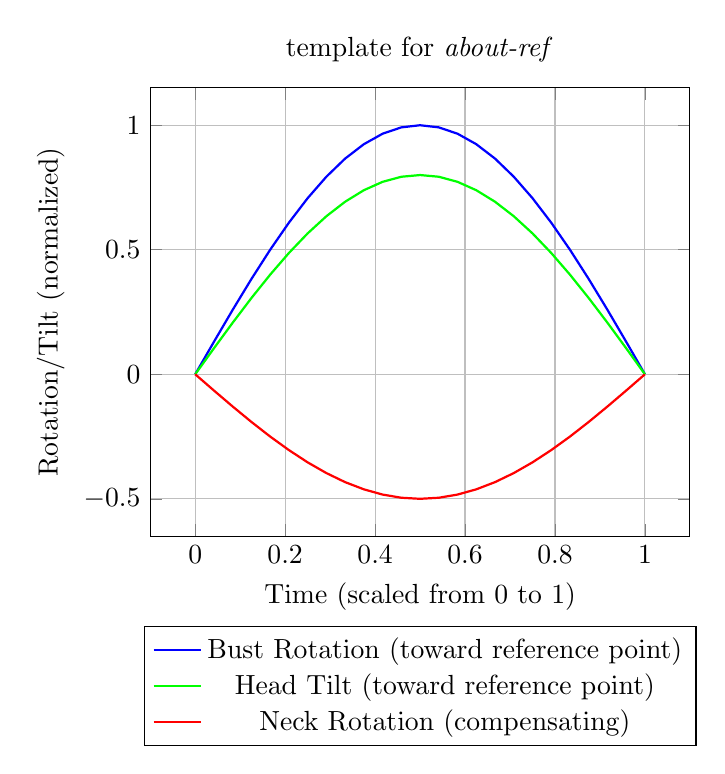
\begin{tikzpicture}
        \begin{axis}[
            title={template for \emph{about-ref}},
            xlabel={Time (scaled from 0 to 1)},
            ylabel={Rotation/Tilt (normalized)},
            grid=major,
            legend style={at={(0.5,-0.2)},anchor=north,legend columns=1} % Legend in two rows
        ]
        % Bust rotation
        \addplot[blue, thick, domain=0:1] {sin(deg(pi*x))};
        \addlegendentry{Bust Rotation (toward reference point)}
        
        % Head tilt
        \addplot[green, thick, domain=0:1] {0.8*sin(deg(pi*x))};
        \addlegendentry{Head Tilt (toward reference point)}
        
        % Neck rotation (compensating)
        \addplot[red, thick, domain=0:1] {-0.5*sin(deg(pi*x))};
        \addlegendentry{Neck Rotation (compensating)}
        
        \end{axis}
    \end{tikzpicture}
    \caption{Artistically Created motion curves for template \emph{about-ref}}
    \label{fig:motion_curves_template_artist}
\end{figure}

\section{Motion Curves}
\label{ch:intermediate_blocks:curves}

Motion curves are a fundamental component of character animation, providing a graphical representation of how a character's movements change over time. By manipulating these curves, animators can control the timing and spacing of movements, ensuring that the animation is realistic and expressive.

\subsection{Skeletal Motion Curves}
\label{ch:intermediate_blocks:curves:skeletal}

The template expression check determines the motion template to be used, which in turn gives us information regarding how a pair of blocks can be connected. However, these motion curves can either effect the skeleton, or the shape keys. For skeleton, these motion curves represent time in x axis, and the joint angle(FK) of the y axis. Each bone has has 4 motion curves (one for each axis of the quaternion rotation).

Figure~\ref{fig:motion_curves_skeletal} shows how motion curves can be used for skeleton for the above example.

\begin{figure}
    \centering \includegraphics[width = 2.5in]{chapters/intermediate_blocks/images/motion_curves_skeletal.png}
    \caption{Motion Curves for Skeleton}
    \label{fig:motion_curves_skeletal}
\end{figure}

\subsection{Shape Key Motion Curves}
\label{ch:intermediate_blocks:curves:shape_keys}

For shape keys, the motion curves represent time in x axis, and the weight of the shape key in the y axis. Each shape key has one motion curve. Figure~\ref{fig:motion_curves_shape_keys} shows how motion curves can be used for shape keys for the facial expressions of the above example.

\begin{figure}
    \centering \includegraphics[width = 2.5in]{chapters/intermediate_blocks/images/motion_curves_shape_keys.png}
    \caption{Motion Curves for Shape Keys}
    \label{fig:motion_curves_shape_keys}
\end{figure}

\section{Results}
\label{ch:intermediate_blocks:results}

Table~\ref{tab:intermediate_blocks_results} shows the results of the intermediate block generation process. Motion curve comparison betweeen standard interpolation and interpolation based on the template for some AZee rules is shown in figure~\ref{tab:intermediate_blocks_comparison}.

\begin{table}
    \centering
    \caption{Intermediate Block Generation Results}
    \begin{tabular}{|c|c|}
    \hline
    \textbf{Azee Rule} & \textbf{Intermediate Blocks Generated with Motion Curve} \\
    \hline
    TODO & \includegraphics[width=1.5in]{chapters/intermediate_blocks/images/template_todo1.png} \\
    \hline
    TODO & \includegraphics[width=1.5in]{chapters/intermediate_blocks/images/template_todo2.png} \\
    \hline
    \end{tabular}
    \label{tab:intermediate_blocks_results}
\end{table}

\begin{figure}
    \centering
    \begin{tabular}{|c|c|}
    \hline
    \textbf{AZee Rule} & \textbf{Standard Interpolation} & \textbf{Template based Interpolation} \\
    \hline
    TODO & \includegraphics[width=1.5in]{chapters/intermediate_blocks/images/standard_interpolation_todo1.png} & \includegraphics[width=1.5in]{chapters/intermediate_blocks/images/template_interpolation_todo1.png} \\
    \hline
    TODO & \includegraphics[width=1.5in]{chapters/intermediate_blocks/images/standard_interpolation_todo2.png} & \includegraphics[width=1.5in]{chapters/intermediate_blocks/images/template_interpolation_todo2.png} \\
    \hline
    \end{tabular}
    \caption{Comparison with normal interpolation}
    \label{tab:intermediate_blocks_comparison}
\end{figure}

The complete animations can be seen in the following video: \url{todo}

An increase in naturalness when animating using the intermediate blocks technique can be seen. Moreover, this work provides us isnights regarding the motion profile which an AZee rule asbtracts.

\section{Conclusion and Future Work}
\label{ch:intermediate_blocks:conclusion_and_future_work}

In this chapter, we explored the generation of intermediate blocks in multi-track representations using motion curves and templates. By leveraging the AZee model and motion curves, we were able to create smooth transitions between constrained blocks, enhancing the naturalness and coherence of Sign Language synthesis. The results demonstrate the effectiveness of this approach compared to using standard block interpolation. 

%limitations
While the current system of motion templates proves effective for generating smooth transitions in most body movements, it faces significant challenges when dealing with finer details such as finger articulation. The complexity of finger movements in sign language, especially during rapid transitions, requires high precision in motion curves and templates. Unfortunately, the current implementation lacks the necessary granularity to handle the intricate dynamics of handshapes and finger configurations, often resulting in unnatural or robotic animations in these areas. Moreover, capturing the nuances of coarticulation between handshapes and other body parts remains an open challenge.

Another limitation stems from too much data in the motion templates. This might bring in information such as the identity of the signer, which may not always generalize well. While procedurally generated templates based on AZee rules offer flexibility, their 

Future areas to improve this technique could include a more detailed quantitative analysis of motion capture data based on a broader range of AZee rules, as well as further refinement of finger tracking and facial expressions in the motion templates.

Future areas to improve this technique could be a deeper quantitative analysis of mocap data based on more AZee rules. This could help in procedurally creating a more robust set of motion templates that can be used across different signing scenarios.

\end{document}
\providecommand{\main}{../..}
\documentclass[../../main]{subfiles}
\begin{document}
\chapter{Facial Expressions}
\label{ch:facial_expressions}

Facial expressions are a crucial element of communication in both spoken and sign languages. In sign languages, they serve a dual purpose: conveying the emotional state of the signer and encoding grammatical information such as questions, negation, and emphasis. While spoken languages rely on tone and intonation for these functions, sign languages depend heavily on non-manual signals, particularly facial expressions, to fully convey the meaning of an utterance. Therefore, creating accurate and expressive facial animations in signing avatars is essential for producing realistic and comprehensible sign language content.

However, synthesizing facial expressions for signing avatars presents significant challenges due to the complexity and subtlety of these expressions. Unlike manual signs, which involve distinct hand and arm movements, facial expressions require the coordinated movement of various facial muscles, each contributing to the overall expression. Different facial features, such as eyebrows, eyes, and mouth, often move independently yet in harmony to produce coherent expressions. Moreover, the same facial expression can convey different meanings depending on the context, adding another layer of complexity to the task.

This chapter tackles these challenges by introducing a method for synthesizing facial expressions using the AZee framework for French Sign Language (LSF). To achieve this, specific production rules for facial expressions were integrated into AZee. By employing action units (AUs) as the foundational elements of these expressions, we can generate blendshapes that precisely represent the required facial movements. These blendshapes are subsequently integrated into a facial rigging system, allowing for the dynamic and realistic animation of signing avatars.

Previous chapters focused on the synthesis of manual features in sign language. In contrast, this chapter centers on the synthesis of facial expressions using the AZee framework, emphasizing their critical role in both emotional communication and the conveyance of grammatical information in sign languages. The precise synthesis of these expressions is therefore essential for enhancing the realism and effectiveness of signing avatars.

The chapter is structured as follows: Section~\ref{ch:facial_expressions:related_work} reviews related work in facial expression synthesis, examining previous approaches, the challenges encountered, and recent advancements. Section~\ref{ch:facial_expressions:related_work:facial_expressions_in_sign_language_synthesis} focuses on the synthesis of facial expressions in sign language avatars, discussing their importance for sign language comprehension and the challenges in capturing their nuances. Section~\ref{ch:facial_expressions:related_work:face_rigging} explores different face rigging techniques, including blendshape-based rigging, skeleton-based rigging, and hybrid methods, and compares their advantages and disadvantages. Finally, Section~\ref{ch:facial_expressions:related_work:emotion_recognition} delves into emotion recognition systems and their role in generating facial expressions that align with the emotional tone of the signed message.

\section{Related Work}
\label{ch:facial_expressions:related_work}

This section reviews the previous work in facial expression synthesis, focusing on the challenges and advancements in capturing the nuances of facial movements. It also discusses the importance of facial expressions in sign language synthesis and the techniques used to model these expressions effectively.

\subsubsection{Facial Expressions Synthesis}
\label{ch:facial_expressions:related_work:facial_expressions_synthesis}

Most of the facial expressions research is motivated by synthesis from voice signals. These methods are generally categorized into lip-sync techniques~\cite{yousaidthat, talkingface, lipmovements, lipsyncexpert}, which align mouth movements with audio, and full-face expression synthesis~\cite{eskimez, greenwood18, controllable_facial_synth}. Some approaches model speaking style with 3D animation parameters~\cite{cudeiro}, create generalized latent audio expressions combined with a person-specific 3D model~\cite{FLAME}, and produce expressive facial outputs conditioned on style, although some are unsuitable for tasks requiring full-face movement~\cite{imitating}. A related work, MakeItTalk~\cite{Yang:2020:MakeItTalk}, introduces a two-stage deep learning model that predicts facial landmark displacements based on audio input and a speaker identifier, followed by an image-to-image translation method to generate the final facial expression. Another study, EAMM~\cite{eamm}, focuses on transferring local emotional deformations to an audio-driven talking face, using deep learning to map audio to keypoints and their dynamics, resulting in emotion-related facial motions.

Synthesis of facial expressions in sign language is a much-less explored area. SGNify~\cite{Forte_2023_CVPR} can do a 3D reconstruction of a signer's face using in FLAME~\cite{FLAME} space from a monocular video. The Paula avatar uses rotational pivots and pre-defined movements, offering more natural and expressive facial animations~\cite{johnson-2022-improved}. More recent work~\cite{azevedo2024empowering} uses sentiment and semantic information to generate realistic facial expressions, achieving state-of-the-art results and outperforming existing approaches. However, these methods are limited in their ability to capture the full range of facial expressions in sign language, particularly the grammatical and emotional nuances that are essential for effective communication. However, these methods are limited in their ability to meaningully relate facial expressions to the signed message.

\subsection{Emotion Recognition}
\label{ch:facial_expressions:related_work:emotion_recognition}

Emotion recognition systems typically use machine learning algorithms to analyze facial features and identify the underlying emotional state. These systems can be trained on large datasets of facial images, which are annotated with emotional labels, to learn the relationships between facial movements and emotions. The most common approach to define emotions is the Ekman's Facial Action Coding System (FACS)~\cite{ekman1978facial}, which categorizes facial expressions into a set of action units (AUs) (figure~\ref{ch:facial_expressions:fig:action_units})  that correspond to specific muscle movements. Recent works by~\cite{luo2022learning} have shown that deep learning models can infer the set of active action units on a face image, which can be used to predict the underlying emotion. EMOCA~\cite{danvevcek2022emoca} is another work which reconstructs 3D faces from single images, accurately capturing emotional expressions by introducing an emotion-consistency loss, significantly improving the quality of reconstructed expressions over previous methods.

\begin{figure}
    \centering
    \includegraphics[width=0.8\textwidth]{chapters/facial_expressions/images/action_units.jpg}
    \caption{Facial Action Coding System (FACS) action units}
    \label{ch:facial_expressions:fig:action_units}
\end{figure}

Emotion recognition can be helpful in understanding as well as modeling facial expressions in sign language synthesis. By analyzing the emotional content of a signed message, we can generate facial expressions that align with the emotional tone of the message, enhancing the realism and expressiveness of the signing avatar.

\subsection{Face Rigging}
\label{ch:facial_expressions:related_work:face_rigging}

Face rigging is the process of creating a digital framework that allows for the animation of facial expressions. There are several approaches to face rigging, each with its advantages and disadvantages. The most common approaches include blendshape-based rigging and skeleton-based rigging.

\subsubsection{Blendshape-Based Rigging}
\label{ch:facial_expressions:related_work:face_rigging:blendshape_based_rigging}

Blendshape-based rigging involves creating a set of predefined facial shapes (blendshapes) that represent various expressions. These blendshapes can be blended together in different proportions to create a wide range of facial expressions. This method is widely used in the animation industry due to its simplicity and flexibility. It allows animators to create complex expressions by adjusting the influence of each blendshape on the final animation. However, the downside of this approach is that it requires a large number of blendshapes to capture all possible expressions, which can be time-consuming to create and manage.

Blendshapes are particularly effective for capturing specific facial movements, such as eyebrow raises, lip curls, cheek puffs, etc. By creating a library of blendshapes that correspond to different facial actions, animators can easily combine these shapes to create expressive and realistic facial animations (figure~\ref{ch:facial_expressions:fig:blendshapes}).

\begin{figure}
    \centering
    \includegraphics[width=0.8\textwidth]{chapters/facial_expressions/images/blendshapes.png}
    \caption{Blendshapes for facial expressions}
    \label{ch:facial_expressions:fig:blendshapes}
\end{figure}

\subsubsection{Skeleton-Based Rigging}
\label{ch:facial_expressions:related_work:face_rigging:skeleton_based_rigging}

Skeleton-based rigging, also known as joint-based rigging, uses a hierarchical system of bones and joints to control facial movements. This approach is more commonly used for animating body movements but can also be applied to facial animation. The advantage of skeleton-based rigging is that it provides more ways to control since the control space of joints can be 3D (figure~\ref{ch:facial_expressions:fig:skeleton_based_rigging}). Example, jaw movements(up, down, left, right, front or back), eye movements, etc. However, it can be less intuitive to work with compared to blendshapes, especially for subtle expressions that require precise control over individual facial muscles.

%todo better diag
\begin{figure}
    \centering
    \includegraphics[width=0.8\textwidth]{chapters/facial_expressions/images/skeleton_based_rigging.png}
    \caption{Skeleton-based rigging for facial expressions}
    \label{ch:facial_expressions:fig:skeleton_based_rigging}
\end{figure}

\subsubsection{Hybrid Rigging}
\label{ch:facial_expressions:related_work:face_rigging:hybrid_rigging}

Hybrid rigging approaches combine elements of both blendshape-based and skeleton-based rigging to offer greater flexibility and control. By leveraging the strengths of both techniques, hybrid rigging can overcome the limitations of each individual approach. For example, blendshapes can be used for fine-tuned expressions, while skeletons provide control over broader movements like jaw or head rotations. 

\subsection{Capturing Facial Expressions}
\label{ch:facial_expressions:related_work:face_rigging:capture}

Manual keyframing and performance-based motion capture are some common means to capture facial expressions .

\subsubsection{Manual Keyframing}
\label{ch:facial_expressions:related_work:face_rigging:capture:manual_keyframing}

Keyframing remains a foundational technique in facial animation, where animators manually set key poses and interpolate between them to create fluid motion. While keyframing is effective in controlled environments, it may struggle to capture the natural variability and complexity required in sign language synthesis, where subtle changes in expression can convey different meanings.

\begin{figure}
    \centering
    \includegraphics[width=0.8\textwidth]{chapters/facial_expressions/images/keyframing.png}
    \caption{Keyframing process, showing how key poses are set and interpolated to create a continuous animation.}
    \label{ch:facial_expressions:fig:keyframing}
\end{figure}

\subsubsection{Performance-Based Motion Capture}
\label{ch:facial_expressions:related_work:face_rigging:capture:performance_based_motion_capture}

Performance-based approaches, such as motion capture, involve capturing real human facial movements and using this data to drive digital avatars. This method provides a high level of realism, capturing the natural dynamics and nuances of facial expressions. Apple's ARKit and FaceCap are examples of performance-based facial animation tools that use motion capture technology to animate digital characters (figure~\ref{ch:facial_expressions:fig:motion_capture}).

\begin{figure}
    \centering
    \includegraphics[width=0.8\textwidth]{chapters/facial_expressions/images/motion_capture.jpg}
    \caption{Performance-based facial animation using Apple's ARKit}
    \label{ch:facial_expressions:fig:motion_capture}
\end{figure}

\section{Action Unit Analysis}
\label{ch:facial_expressions:action_unit_analysis}

Our method for facial expression synthesis is based on first formalizing the AZee facial expression rules in terms of action units (AUs). This section outlines the steps involved in our method, from the analysis of action units to the creation of blendshapes and the generation of motion curves.

AUs represent the activation of specific facial muscles and are the basic components of facial expressions. Each AU corresponds to a particular movement, such as raising the eyebrows or pursing the lips, and can be combined with other AUs to create complex expressions.

To analyze AUs, we used a combination of manual observation and automatic detection tools.

\subsection{Automatic detection}
\label{ch:facial_expressions:action_unit_analysis:automatic_detection}

We the AU detector by~\cite{luo2022learning} on mediapipe extractions of still images (figure~\ref{ch:facial_expressions:fig:face_detect}).

%todo more detailed diagram(images -> mediapipe -> AU detector)
\begin{figure}
    \centering
    \includegraphics[width=0.8\textwidth]{chapters/facial_expressions/images/face_detect.png}
    \caption{Facial action unit detection using mediapipe and the AU detector by~\cite{luo2022learning} for \emph{big-threatening}}
    \label{ch:facial_expressions:fig:face_detect}
\end{figure}

While it is a good starting point, manual adjustments were required by a linguist to ensure accuracy.

\subsection{Automatic detection}
\label{ch:facial_expressions:action_unit_analysis:automatic_detection}

We used a linguists input by adjusting the movements of individual facial features for each expression(figure~\ref{ch:facial_expressions:fig:face_adjust}).

% todo face adjust diagram(example medaipe AU face retargeted on a template mesh, then adjusted by a linguist)
\begin{figure}
    \centering
    \includegraphics[width=0.8\textwidth]{chapters/facial_expressions/images/face_adjust.png}
    \caption{Manual adjustment of facial expressions to ensure accuracy.}
    \label{ch:facial_expressions:fig:face_adjust}
\end{figure}

The synthesized facial expressions were taken from our reference corpus (the 40 brèves corpus)~\cite{challant2024extending, challant2022first}, breaking down each expression into its constituent AUs. This approach allowed us to ensure that our blendshapes accurately reflected the intended expressions, capturing both the emotional and grammatical nuances required for sign language synthesis.

\section{Blendshape Creation}
\label{ch:facial_expressions:blendshape_creation}

Once the AUs were identified, we used FACSHuman~\cite{gilbert2021facshuman} blendshapes as reference to create shapekeys in blender that correspond to each AU (figure~\ref{ch:facial_expressions:fig:facshuman_blendshapes}). Shape keys (figure~\ref{ch:facial_expressions:fig:shape_keys}) are essentially different versions of a 3D model, each representing a specific change in vertices. By blending and interpolating these keys together, we can create a wide range of mesh shapes.

Since the FACSHuman blendshape work on any MakeHuman template mesh, this technique of synthesis is avatar independant. However, since the original model doesn't cover all the blendshapes(for all the face meshes), some blendshapes were created manually. The complete process involved iterating between manual adjustments and automated tools to ensure that the blendshapes accurately captured the intended expressions. The creation of blendshapes also involved ensuring that they could be seamlessly combined to create complex expressions. For example, the blendshape for AU4 (Brow Lowerer) was designed to work in conjunction with AU6 (Cheek Raiser) and AU12 (Lip Corner Puller) to create expressions of anger or determination. This required careful coordination of the vertex movements across different blendshapes to avoid unnatural deformations or artifacts in the final animation.

\begin{figure}
    \centering
    \includegraphics[width=0.8\textwidth]{chapters/facial_expressions/images/facshuman_blendshapes.png}
    \caption{FACSHuman blendshapes used as reference for creating shapekeys in blender.}
    \label{ch:facial_expressions:fig:facshuman_blendshapes}
\end{figure}

\begin{figure}
    \centering
    \includegraphics[width=0.8\textwidth]{chapters/facial_expressions/images/shape_keys.png}
    \caption{Blender interface. (a) Shape Key properties (b) 3D Viewport (c) Non-linear Editor (d) Action Editor (e) AZee editor}
    \label{ch:facial_expressions:fig:shape_keys}
\end{figure}

Lastly, we extended the low-level AZee language morph set with 94 blendshapes corresponding to most of the action units in the FACS system (figure~\ref{tab:added_units}) along with some additional blendshapes for the tongue. A few action units were not added~\ref{tab:not_added} since they were controlled by other skeletal constraints. Some morphs are also alternative blendshapes for the same action unit~\ref{tab:alternative_blendshapes} but with a different effect on the face.

\begin{table}[h]
    \centering
    \scriptsize
    \begin{tabular}{|c|l|c|l|}
        \hline
        \textbf{AU Code} & \textbf{Description}                     & \textbf{AU Code} & \textbf{Description}                      \\ \hline
        AU1              & Inner Brow Raise                        & AU1\_L            & Inner Brow Raise (Left)                   \\ \hline
        AU1\_R           & Inner Brow Raise (Right)                & AU2              & Outer Brow Raise                          \\ \hline
        AU2\_L           & Outer Brow Raise (Left)                 & AU2\_R            & Outer Brow Raise (Right)                  \\ \hline
        AU4              & Brow Lowerer                            & AU5              & Upper Lid Raise                           \\ \hline
        AU5\_L           & Upper Lid Raise (Left)                  & AU5\_R            & Upper Lid Raise (Right)                   \\ \hline
        AU6              & Cheek Raise                             & AU6\_L            & Cheek Raise (Left)                        \\ \hline
        AU6\_R           & Cheek Raise (Right)                     & AU7              & Lids Tight                                \\ \hline
        AU7\_L           & Lids Tight (Left)                       & AU7\_R            & Lids Tight (Right)                        \\ \hline
        AU8              & Lips Toward Each Other                  & AU9              & Nose Wrinkle                              \\ \hline
        AU9\_L           & Nose Wrinkle (Left)                     & AU9\_R            & Nose Wrinkle (Right)                      \\ \hline
        AU10             & Upper Lip Raiser                        & AU10\_L           & Upper Lip Raiser (Left)                   \\ \hline
        AU10\_R          & Upper Lip Raiser (Right)                & AU11             & Nasolabial Furrow Deepener                \\ \hline
        AU11\_L          & Nasolabial Furrow Deepener (Left)       & AU11\_R           & Nasolabial Furrow Deepener (Right)        \\ \hline
        AU12             & Lip Corner Puller                       & AU12\_L           & Lip Corner Puller (Left)                  \\ \hline
        AU12\_R          & Lip Corner Puller (Right)               & AU13             & Sharp Lip Puller                          \\ \hline
        AU13\_L          & Sharp Lip Puller (Left)                 & AU13\_R           & Sharp Lip Puller (Right)                  \\ \hline
        AU14             & Dimpler                                 & AU14\_L           & Dimpler (Left)                            \\ \hline
        AU14\_R          & Dimpler (Right)                         & AU15             & Lip Corner Depressor                      \\ \hline
        AU15\_L          & Lip Corner Depressor (Left)             & AU15\_R           & Lip Corner Depressor (Right)              \\ \hline
        AU16             & Lower Lip Depress                       & AU17             & Chin Raiser                               \\ \hline
        AU18             & Lip Pucker                              & AU19             & Tongue Show                               \\ \hline
        AU20             & Lip Stretch                             & AU20\_L           & Lip Stretch (Left)                        \\ \hline
        AU20\_R          & Lip Stretch (Right)                     & AU21             & Neck Tightener                            \\ \hline
        AU22\_25\_up\_down & Lip Funneler (Both Lips) & AU23             & Lip Tightener                             \\ \hline
        AU24             & Lip Presser                             & AU25             & Lips Part                                 \\ \hline
        AU25\_L          & Lips Part (Left)                        & AU25\_R           & Lips Part (Right)                         \\ \hline
        AU26             & Jaw Drop                                & AU27             & Mouth Stretch                             \\ \hline
        AU28             & Lips Suck                               & AU29             & Jaw Thrust                                \\ \hline
        AU30\_L          & Jaw Sideways (Left)                     & AU30\_R           & Jaw Sideways (Right)                      \\ \hline
        AU31             & Jaw Clencher                            & AU32             & Bite                                      \\ \hline
        AU33             & Blow                                    & AU34             & Puff                                      \\ \hline
        AU35             & Cheek Suck                              & AU36             & Tongue Bulge                              \\ \hline
        AU37             & Lip Wipe                                & AU38             & Nostril Dilate                            \\ \hline
        AU39             & Nostril Compress                        & AU43             & Eye Closure                               \\ \hline
        AU43\_L          & Eye Close (Left)                        & AU43\_R           & Eye Close (Right)                         \\ \hline
    \end{tabular}
    \caption{Added blend shapes} 
    \label{tab:added_units} 
\end{table}

\begin{table}
    \centering
    \scriptsize
    \begin{tabular}{|c|l|c|l|}
        \hline
        \textbf{AU Code} & \textbf{Description}                     & \textbf{AU Code} & \textbf{Description}                      \\ \hline
        AU40             & Sniff                                   & AU41             & Lid Droop                                 \\ \hline
        AU42             & Slit                                    & AU44             & Squint                                    \\ \hline
        AU45             & Blink                                   & AU46             & Wink                                      \\ \hline
        AU51             & Head Turn Left (IK controlled)          & AU52             & Head Turn Right (IK controlled)           \\ \hline
        AU53             & Head Up (IK controlled)                 & AU54             & Head Down (IK controlled)                 \\ \hline
        AU55             & Head Tilt Left (IK controlled)          & AU56             & Head Tilt Right (IK controlled)           \\ \hline
        AU57             & Head Forward (IK controlled)            & AU58             & Head Back (IK controlled)                 \\ \hline
        AU61             & Eyes Turn Left (lookat constraint)      & AU62             & Eyes Turn Right (lookat constraint)       \\ \hline
        AU63             & Eyes Up (lookat constraint)             & AU64             & Eyes Down (lookat constraint)             \\ \hline
    \end{tabular}
    \caption{Action units skipped} 
    \label{tab:not_added} 
\end{table}


\vspace{1cm}

\begin{table}
    \centering
    \scriptsize
    \begin{tabular}{|c|l|c|l|}
        \hline
        \textbf{AU Code} & \textbf{Description}                     & \textbf{AU Code} & \textbf{Description}                      \\ \hline
        AU1\_a            & Inner Brow Raise (Alternative)          & AU2\_a            & Outer Brow Raise (Alternative)           \\ \hline
        AU4\_a            & Brow Lowerer (Alternative A)            & AU4\_b            & Brow Lowerer (Alternative B)             \\ \hline
        AU6\_a            & Cheek Raise (Alternative A)             & AU6\_b            & Cheek Raise (Alternative B)              \\ \hline
        AU9\_a            & Nose Wrinkle (Alternative A)            & AU12\_a           & Lip Corner Puller (Alternative A)        \\ \hline
        AU12\_b           & Lip Corner Puller (Alternative B)       & AU17\_a           & Chin Raiser (Alternative A)              \\ \hline
        AU18\_a           & Lip Pucker (Alternative)                & AU25\_a           & Lips Part (Alternative A)                \\ \hline
        AU22\_25\_upper  & Lip Funneler (Upper Lip)     & AU22\_25\_down   & Lip Funneler (Bottom Lip)  \\ \hline
        AU26\_lip\_down   & Jaw Drop Bottom Lip Down (Alternative)  & AU26\_tongue\_down & Jaw Drop Tongue Down (Alternative)       \\ \hline
        AU26\_tongue\_out & Jaw Drop Tongue Out (Alternative)       & AU26\_a           & Jaw Drop (Alternative)                   \\ \hline
        AU28\_a           & Lips Suck (Upper Lip)                   & AU28\_bottom      & Lips Suck (Lower Lip)                    \\ \hline
        tongue\_back\_up  & Tongue Back Up                          & tongue\_out       & Tongue Out                               \\ \hline
        tongue\_up        & Tongue Up                               & tongue\_wide      & Tongue Wide                              \\ \hline
    \end{tabular}
    \caption{Alternative blend shapes} 
    \label{tab:alternative_blendshapes}
\end{table}



\subsection{Motion Curves for Blendshapes}
\label{ch:facial_expressions:motion_curves_for_blendshapes}

After creating the blendshapes, we generated motion curves (more discussed in chapter~\ref{ch:intermediate_blocks}) to control how these shapes are animated over time. Motion curves define the changes in the blendshape's influence over the course of an animation, allowing for smooth transitions between different facial expressions.

We extended our intermediate block generation algorithm to include motion curves for facial morphs. This involved creating additional curves that specify the timing and intensity of facial movements based on the template. By controlling the acceleration and deceleration of these movements, we were able to create more naturalistic animations that reflect the dynamic nature of facial expressions.

For example, in the expression "big-threatening," the motion curves were designed to gradually increase the influence of the blendshapes corresponding to AU10 (Upper Lip Raiser) and AU25 (Lips Part) while simultaneously decreasing the influence of AU4 (Brow Lowerer) as the expression transitions from a neutral state to one of aggression (figure~\ref{ch:facial_expressions:fig:motion_curve_example}). This careful modulation of the blendshape influences over time resulted in an expression that not only looked realistic but also conveyed the intended emotional and grammatical cues effectively.

\begin{figure}
    \centering
    \includegraphics[width=0.8\textwidth]{chapters/facial_expressions/images/motion_curve_example.png}
    \caption{Motion curves controlling the blendshape influences for the expression "big-threatening."}
    \label{ch:facial_expressions:fig:motion_curve_example}
\end{figure}

%todo metahuman, flame, etc.

\section{Results and Evaluation}
\label{ch:facial_expressions:results}

Synthesis of all the facial expressions from the 40 brèves corpus can be seen in table~\ref{tab:facial_expressions}. The expressions were created by combining the relevant blendshapes to produce realistic and expressive facial animations.

% todo finish table
\begin{table}
    \centering
    \begin{tabular}{|c|c|c|}
        \hline
        \textbf{Expression} & \textbf{Description} & \textbf{Blendshapes} \\
        \hline
        AZee & Facial Expression \\
        todo & todo \\
    \end{tabular}
    \caption{Facial expressions synthesized using the AZee framework.}
    \label{tab:facial_expressions}
\end{table}

\section{Evaluation}
\label{ch:facial_expressions:evaluation}

Table~\ref{tab:facial_expressions_evaluation} shows the subjective evaluation by a linguist of the facial expressions synthesized using the AZee framework. The expressions were assessed based on their accuracy, expressiveness, and effectiveness in conveying the intended emotional and grammatical cues.

\begin{table*}
    \centering
    \begin{tabular}{|l|p{8cm}|}
    \hline
    \textbf{Expression} & \textbf{Limitations} \\
    \hline
    \texttt{almost-reaching} & Mouth modeling unconvincing. \\
    \hline
    \texttt{continuously} & "Pffff" air and cheek puff difficult, neutral eyebrows. \\
    \hline
    \texttt{do-you-realise} & Thick eyebrow issue. \\
    \hline
    \texttt{it-is-a-shame} & Mouth expression not quite real. \\
    \hline
    \texttt{most-probably} & Less visible teeth preferred, thick eyebrow issue. \\
    \hline
    \texttt{much-almost-too-much} & Frowning eyebrows and lack of eye wrinkles not convincing. \\
    \hline
    \texttt{nothing-sticks-out} & Tucked lips difficult to model. \\
    \hline
   \texttt{something-sticks-out} & Interpreted as confusion, mouth modeling limitation. \\
    \hline
    \texttt{trouble-disturbance} & Frowning eyebrows difficult, mouth "rising" hard to model, result not convincing. \\
    \hline
    \texttt{uneasy-awkward} & Tongue tip out with slightly open mouth hard to model, unconvincing. \\
    \hline
    \texttt{with-chaos} & Single cheek blow/puff and alternating eye blinks hard without animation. \\
    \hline
    \texttt{with-no-precision} & Upper lip over lower and mouth near nose unmodellable. \\
    \hline
    \texttt{with-surprise} & Cannot lower lower eyelid fully, thick eyebrow issue. \\
    \hline
    \texttt{with-uncertainty} & Appears sadder than uncertain, thick eyebrow issue. \\
    \hline
    \texttt{with-worry} & Lack of wrinkles around nose/forehead. \\
    \hline
    \end{tabular}
    \caption{Limitations for each facial expression rule.}
    \label{tab:facial_expressions_evaluation}
\end{table*}

We observe that expressions that involved subtle mouth movements, such as "it-is-a-shame" or "something-sticks-out," were more challenging to model accurately, highlighting areas for further refinement.

Table~\ref{tab:facial_expressions_quantitative} shows the quantitative evaluation of the facial expressions using the Frechet Expression Distance (FED). We also fitted FLAME~\cite{FLAME} on the ground truth facial expressions~\ref{ch:facial_expressions:fig:spectre} and compared them to the expressions synthesized using our method framework. The FED scores provide a measure of the similarity between the ground truth and synthesized expressions, with lower scores indicating a closer match.

\begin{figure}
    \centering
    \includegraphics[width=0.8\textwidth]{chapters/facial_expressions/images/sgnify.png}
    \caption{Facial expressions generated using FLAME by fitting SPECTRE}
    \label{ch:facial_expressions:fig:spectre}
\end{figure}

\begin{table}
    \centering
    \begin{tabular}{|c|c|}
        \hline
        \textbf{Expression} & \textbf{FED Score} \\
        \hline
        big-threatening & todo \\
        \hline
    \end{tabular}
    \caption{Quantitative evaluation of facial expressions synthesized}
    \label{tab:facial_expressions_quantitative}
\end{table}

The FED scores indicate that the synthesized expressions closely matched the ground truth expressions, demonstrating the effectiveness of our method in capturing the nuances of facial movements.

We also compare the synthesized utterance (with facial expressions) with the original utterance (without facial expressions) to evaluate the impact of facial expressions on sign language comprehension. For this we synthesize the following AZee description.

\begin{verbatim}    
    todo
\end{verbatim}

The following link shows the comparison between the two versions (and the SGNify version for inference) of the utterance: \href{todo}. We observe that the added facial expressions todo...

\section{Conclusion}
\label{ch:facial_expressions:conclusion}

Facial expressions play a crucial role in sign language communication, conveying both emotional and grammatical information. In this chapter, we presented a method for synthesizing facial expressions using the AZee framework, focusing on the creation of blendshapes from action units (AUs) and the generation of motion curves to control these shapes over time. Our method involved analyzing AUs from the FACS system, creating blendshapes based on these AUs, and generating motion curves to animate the blendshapes. The synthesized facial expressions were evaluated subjectively by a linguist and quantitatively using the Frechet Expression Distance (FED) metric, demonstrating the effectiveness of our method in capturing the nuances of facial movements. The results show that the synthesized expressions closely matched the ground truth expressions, highlighting the potential of our method for enhancing the realism and expressiveness of signing avatars. Future work will focus on refining the blendshapes and motion curves to improve the accuracy and naturalness of the facial expressions, as well as exploring the integration of emotion recognition systems to generate facial expressions that align with the emotional tone of the signed message. By continuing to develop and refine our method, we aim to create more realistic and effective facial animations for sign language synthesis, enhancing the overall quality and accessibility of sign language content.


\end{document}
\documentclass[../../main.tex]{subfiles}
\begin{document}
\chapter{Motion Matching for Sign Language Synthesis}
\label{ch:motion_matching}

In the previous chapters, we looked at granularity in sign language animation based on AZee's structure. However, one of the key missing pieces in our study was the ability to shortcut or match a posture state on generated poses. Motion matching is a technique that aims to address this challenge by matching the motion of a character to a set of predefined poses or movements. By comparing the motion of the character to a database of motion data, motion matching can generate more realistic and contextually appropriate animations.

The past decade has seen a rise in deep learning technologies in in the field of character animation. These technologies have been used to generate realistic and expressive animations for a wide range of applications, from video games to virtual reality. One of the key challenges in character animation is the generation of natural and fluid motion, which requires the ability to capture the nuances of human movement and behavior. 

In this work, we focus on the development of a motion matching system for sign language using a pose prior model derived from a sign language dataset. The pose prior model captures the typical poses and movements associated with different signs, providing a statistical framework that guides the motion matching process. By learning these priors from a large dataset, our system is able to generate realistic and contextually appropriate sign language gestures in real time.

In this chapter, section 

\section{Related work}
\label{ch:motion_matching:related_work}

In this section, we discuss relevant background work in motion matching, focusing on classical methods, data-driven approaches, and the integration of latent space representations. These methodologies form the foundation for understanding advancements in character animation.

\subsection{Classical Inverse Kinematics (IK) Methods}
\label{ch:motion_matching:related_work:classical_ik}

Classical Inverse Kinematics (IK) methods have been a cornerstone in the field of character animation, providing techniques to determine the necessary joint angles to achieve a desired end-effector position. Some of these methods are Jacobian-based approach \cite{TODO itasc}, Cyclic Coordinate Descent (CCD)\cite{TODO}, and Forward And Backward Reaching Inverse Kinematics (FABRIK)\cite{TODO}.

Jacobian-Based Methods involve computing the Jacobian matrix to linearize the relationship between joint angles and end-effector positions. By iteratively adjusting joint angles to reduce the error between the current and target positions, these methods offer a robust solution for real-time applications\ref{fig:jacobian_based}. However, they often require complex matrix operations and are sensitive to singularities, making them less suitable for more complex animations [TODO].

\begin{figure}
    \centering \includegraphics[width = 2.5in]{chapters/motion_matching/images/jacobian_based.png}
    \caption{Jacobian based(iTasC) IK solving}
    \label{fig:jacobian_based}
\end{figure}

Cyclic Coordinate Descent (CCD) simplifies the IK problem by iteratively adjusting one joint at a time, minimizing the distance between the end-effector and the target\ref{fig:ccdik}. CCD is computationally efficient and easy to implement, making it popular in game engines. However, its greedy approach can lead to suboptimal solutions, especially in highly constrained scenarios\cite{TODO}.

\begin{figure}
  \centering \includegraphics[width = 2.5in]{chapters/motion_matching/images/ccdik.png}
  \caption{Cyclic Coordinate Descent (CCD) IK solving}
  \label{fig:ccdik}
\end{figure}

FABRIK differs from other methods by focusing on the positions of joints rather than their angles. It iteratively adjusts the positions of joints through a two-pass approach, first from the end-effector to the root and then from the root to the end-effector\ref{fig:fabrik}. This method is known for its simplicity and stability, particularly in scenarios where maintaining a natural joint configuration is crucial\cite{TODO}.

\begin{figure}
  \centering \includegraphics[width = 2.5in]{chapters/motion_matching/images/fabrik.png}
  \caption{Forward And Backward Reaching Inverse Kinematics(FABRIK) solving}
  \label{fig:fabrik}
\end{figure}

These classical methods have been widely adopted due to their balance between computational efficiency and control, making them suitable for a variety of real-time applications. However, they have notable limitations. They are prone to singularities, where solutions become unstable, and often require significant computational resources, especially in complex or high-dimensional systems. The resulting movements can sometimes be unnatural or biomechanically unrealistic, particularly when handling joint limits or multiple end-effectors. Additionally, these methods struggle with complex constraints and often produce suboptimal solutions that may not adapt well to varying scenarios, making them less suitable for dynamic or highly detailed applications \ref{fig:problems_classical}.

\begin{figure}
  \centering \includegraphics[width = 2.5in]{chapters/motion_matching/images/problems_classical.png}
  \caption{Problems with classical IK solving methods}
  \label{fig:problems_classical}
\end{figure}

\subsection{Data-Driven IK Approaches}
\label{ch:motion_matching:related_work:data_driven_ik}

The limitations of classical IK methods have spurred the development of data-driven approaches, which leverage large datasets and machine learning to improve the realism and flexibility of character animations.

Motion Matching represents a significant shift from traditional IK by utilizing a large database of motion capture (mocap) data. Instead of predefined animation clips, Motion Matching dynamically selects the most appropriate pose based on user inputs and contextual parameters. This approach was notably employed by Ubisoft in the game For Honor, where it enabled more fluid and responsive character animations\ref{fig:for_honor}. Motion Matching's ability to break down animations into fine-grained clips allows for seamless transitions and more natural movements\cite{TODO}.

\begin{figure}
  \centering \includegraphics[width = 2.5in]{chapters/motion_matching/images/for_honor.png}
  \caption{Motion Matching in For Honor}
  \label{fig:for_honor}
\end{figure}

Phase-Functioned Neural Networks (PFNN) \cite{TODO} extends the capabilities of motion matching by incorporating phase information into the neural network's weights. This phase-aware approach allows the network to generate contextually appropriate animations that account for the cyclical nature of bipedal movement, such as walking or running. Unlike traditional methods that rely on blending animation clips, PFNN encodes the entire animation process within the neural network, offering greater flexibility and control.

\begin{figure}
  \centering \includegraphics[width = 2.5in]{chapters/motion_matching/images/pfnn.png}
  \caption{Phase-Functioned Neural Networks (PFNN) for motion matching}
  \label{fig:pfnn}
\end{figure}

Style-Based Inverse Kinematics (Style IK) leverages machine learning to represent poses in a latent space, where the distribution of poses can be learned and sampled. Using Scaled Gaussian Process Latent Variable Models (SGPLVM), Style IK can generate stylized animations that conform to specific aesthetic or functional constraints. This approach is particularly useful for creating animations that need to adhere to a particular style or where mocap data is not available\cite{TODO}.

\begin{figure}
  \centering \includegraphics[width = 2.5in]{chapters/motion_matching/images/style_ik.png}
  \caption{Pose in latent space using Style IK}
  \label{fig:style_ik}
\end{figure}

These data-driven approaches represent a significant advancement over classical IK methods, offering greater flexibility, realism, and the ability to handle complex, non-linear constraints. However, they also introduce new challenges, such as the need for extensive training data and increased computational demands, particularly in real-time applications \ref{fig:problem_data_driven}.

\begin{figure}
  \centering \includegraphics[width = 2.5in]{chapters/motion_matching/images/problem_data_driven.png}
  \caption{TODO}
  \label{fig:problem_data_driven}
\end{figure}

\subsection{Latent Space Representations in Animation}
\label{ch:motion_matching:related_work:latent_space}

Latent space representations have become increasingly important in character animation, providing a powerful tool for managing the complexity of pose and motion data. Variational Autoencoders (VAEs)\cite{TODO}, such as the one used in SMPLify-X\cite{TODO}, learn a probabilistic model of human poses, allowing for the generation and manipulation of poses in a lower-dimensional space. In the context of pose estimation, VAEs help in predicting 3D poses from 2D images by learning a latent space that captures the distribution of plausible human poses. This latent space can then be sampled to generate realistic poses that meet specific constraints, such as end-effector positions or overall body posture\ref{fig:simplifyx}.

\begin{figure}
  \centering \includegraphics[width = 2.5in]{chapters/motion_matching/images/simplifyx.png}
  \caption{SMPLify-X}
  \label{fig:simplifyx}
\end{figure}

The use of latent space not only reduces the dimensionality of the data, making it easier to work with, but also enables more sophisticated manipulations, such as style transfer or the synthesis of new poses that blend characteristics from multiple examples. This has proven particularly valuable in scenarios where high-quality mocap data is not available, or where the goal is to create stylized or non-standard animations.

VPoser\cite{TODO}, a specific implementation of a VAE, further demonstrates the power of latent space in animation. By encoding poses into a low-dimensional latent space, VPoser can be used in optimization processes to ensure that generated poses are both realistic and meet specific criteria. This approach is particularly effective in applications like pose estimation from monocular images, where the latent space helps to regularize the solution and avoid physically implausible poses.

Overall, latent space representations have become a crucial component of modern character animation, enabling more complex and realistic animations while also providing tools for creative control and manipulation.

\section{Motion Matching with AZee Low Level synthesis}
\label{ch:motion_matching:motion_matching_with_azee}

In this section, we discuss the application of motion matching techniques to the AZee low-level synthesis system. By integrating motion matching, data-driven IK, and latent space representations into the AZee framework, we aim to enhance the realism and expressiveness of sign language animations.

\subsection{Preparing the dataset}
\label{ch:motion_matching:motion_matching_with_azee:dataset}

The first step in integrating motion matching into AZee is to train a Variational Autoencoder (VAE) on set of sign language poses. For this task, we use a dataset of mocap data collected from the Rosetta dataset \cite{TODO}. The dataset consists of todo poses and should capture the diversity of poses and movements associated with different signs, providing a rich source of training data for the VAE.. Since our focus was only on the upper body, we didn't use the facial bones and the lower body for the training. We also retargeted the mocap data to the BAZeel avatar, which is compatible with the AZee skeleton structure (figure \ref{fig:retargeted}).

\begin{figure}
  \centering \includegraphics[width = 2.5in]{chapters/motion_matching/images/retargeted.png}
  \caption{Retargeted mocap data to BAZeel avatar}
  \label{fig:retargeted}
\end{figure}

Next, we converted the motion into AZee's FK pose array. The FK pose array consists of the rotation values of each joint in the AZee skeleton (figure \ref{fig:azee_fk_pose}). This representation is more suitable for the VAE training process, as it captures the pose information in a compact and standardized format.

\begin{figure}
  \centering \includegraphics[width = 2.5in]{chapters/motion_matching/images/azee_fk_pose.png}
  \caption{AZee FK Pose Array}
  \label{fig:azee_fk_pose}
\end{figure}

\subsection{Training VPoser}
\label{ch:motion_matching:motion_matching_with_azee:training}

A VAE \cite{todo} is a type of generative model that learns a low-dimensional latent space representation of the input data. In the context of character animation, a VAE can be used to capture the distribution of poses in a dataset, allowing for the generation of new poses that are statistically similar to the training data. The VAE consists of an encoder network that maps input poses to a latent space and a decoder network that reconstructs the input poses from the latent space (figure \ref{fig:vae}).

\begin{figure}
  \centering \includegraphics[width = 2.5in]{chapters/motion_matching/images/vae.png}
  \caption{Variational Autoencoder (VAE)}
  \label{fig:vae}
\end{figure}

VPoser is a specific implementation of a VAE designed for pose estimation and synthesis. We train the VPoser using the AZee FK pose array data. The training ...todo

\subsection{Implementing Motion Matching}
\label{ch:motion_matching:motion_matching_with_azee:implementation}

With the VAE trained, we can now implement a motion matching system that leverages the learned latent space to match poses generated by the AZee system to the most appropriate pose in the dataset (figure \ref{fig:motion_matching}).

\begin{figure}
  \centering \includegraphics[width = 2.5in]{chapters/motion_matching/images/motion_matching.png}
  \caption{Motion Matching with VAE}
  \label{fig:motion_matching}
\end{figure}

Algorithm \ref{alg:motion_matching} outlines the motion matching process. Given a target pose generated by the AZee synthesizor, we first encode the pose into the latent space using the VPoser encoder. We then compute the distance between the encoded pose and each pose in the dataset, selecting the pose with the smallest distance as the best match. Finally, we decode the matched pose back into the AZee FK pose array and apply it to the character.

todo
\begin{algorithm}
  \caption{Motion Matching Algorithm}
  \label{alg:motion_matching}
  \begin{algorithmic}
    \STATE \textbf{Input:} Target pose $P_{target}$
    \STATE \textbf{Output:} Matched pose $P_{matched}$
    \STATE Encode $P_{target}$ into latent space: $z_{target} = \text{VPoser.encoder}(P_{target})$
    \STATE $P_{matched} = \text{argmin}_{P_i} \text{dist}(z_{target}, \text{VPoser.encoder}(P_i))$
    \STATE $P_{matched} = \text{VPoser.decoder}(z_{matched})$
    \STATE Apply $P_{matched}$ to character
  \end{algorithmic}
\end{algorithm}

\subsection{Results and Evaluation}
\label{ch:motion_matching:motion_matching_with_azee:results}

Snapshots with standard synthesis and motion matching synthesis and the corresponding AZee code for the same are shown in table \ref{tab:results}.

\begin{table}
  \centering
  \begin{tabular}{|c|c|c|}
    \hline
    \textbf{Standard Synthesis} & \textbf{Motion Matching Synthesis} & \textbf{AZee Code} \\
    \hline
    \includegraphics[width = 1.5in]{chapters/motion_matching/images/standard_synthesis.png} & \includegraphics[width = 1.5in]{chapters/motion_matching/images/motion_matching_synthesis.png} & \begin{lstlisting}
      AZeePose pose = AZeeSynthesize();
      AZeeMotionMatch(pose);
    \end{lstlisting} \\
    \hline
  \end{tabular}
  \caption{Results of Motion Matching Synthesis}
  \label{tab:results}
\end{table}

The synthesized videos can also be viewed at \href{todo}.

Initial subjective evaluations suggest that the motion matching system produces more natural and contextually appropriate animations compared to standard synthesis. However, due to the lack of good quality mocap data, the integration of motin matching into Sign Language synthesis is still in the early stages. We also observe that the system can change the pose of the character in a way that is not always desirable \ref{fig:problem_motion_matching}.

\begin{figure}
  \centering \includegraphics[width = 2.5in]{chapters/motion_matching/images/problem_motion_matching.png}
  \caption{Problems with motion matching}
  \label{fig:problem_motion_matching}
\end{figure}

Lastly, figure \ref{fig:losses} shows how retargeting the mocap data to the AZee skeleton structure results in a loss of information. This loss can affect the quality of the generated animations and is an area for future improvement.

\begin{figure}
  \centering \includegraphics[width = 2.5in]{chapters/motion_matching/images/losses.png}
  \caption{Losses in retargeting mocap data}
  \label{fig:losses}
\end{figure}

\section{Discussion}
\label{ch:motion_matching:discussion}

The integration of motion matching into the AZee system represents a significant advancement in sign language synthesis. By leveraging data-driven IK and latent space representations, we are able to generate more realistic and contextually appropriate sign language animations. This has the potential to enhance the expressiveness and naturalness of sign language avatars, making them more engaging and accessible to users. In some ways, this offfers a new perspective to Sign Language synthesis where the linguistics decides the "what" and the motion matching decides the "how" of the animation.

While the integration of machine learning into SL synthesis offers numerous advantages, it also introduces new challenges. Data-driven and latent space methods typically require significant computational resources, both during training and inference. This can be a major barrier in real-time applications, where low latency is critical. Also the effectiveness of machine learning models depends heavily on the availability of high-quality training data. In many cases, obtaining sufficient mocap data can be difficult, especially for non-standard or stylized animations. Lastly, while machine learning models can generate realistic and high-quality animations, they often lack the fine-grained control that human animators require. Ensuring that these models produce outputs that align with artistic vision remains a significant challenge.

\end{document}
\documentclass[../../main.tex]{subfiles}
\begin{document}
\chapter{Conclusion}
\label{ch:conclusion}

In this chapter, we present a summary and overview of the contributions made in this thesis on \textit{\gls{sl} Synthesis by a Decreasing Granularity System from AZee}. We outline the research conducted throughout the thesis in Section~\ref{ch:conclusion:summary}. todo

\section{Summary}
\label{ch:conclusion:summary}

This thesis explores innovative approaches to synthesizing \gls{sl} using a decreasing granularity system based on the AZee framework. The primary objective was to develop a system that could generate \gls{sl} sequences that are linguistically accurate and easier to reproduce, addressing a crucial need in accessible communication technologies for the Deaf and Hard of Hearing communities.

In Chapter~\ref{ch:background_work}, we reviewed the foundational work in describing \gls{sl}s, and synthesis techniques, particularly focusing on synthesis from AZee. AZee provides a structured way to describe \gls{sl} at varying levels of granularity. However, existing methods often struggle to balance linguistic accuracy with ease of synthesis. 

Chapter~\ref{ch:avatar_creation_pose_synthesis} introduced a layered rigging system for signing avatars, emphasizing the importance of rigging in realistic character animation. It presented a procedural rigging system tailored for \gls{sl} gestures, focusing on the upper body. The chapter discussed automating site generation using a raycasting algorithm and improving the rigging process with deformation, inverse kinematics (IK), and forward kinematics (FK) layers. It also introduced constraint-based posture optimization and morph constraints. Finally, the chapter evaluated the system’s performance, accuracy, and animation quality, highlighting the potential for future enhancements in \gls{sl} avatar animation. 

In Chapter~\ref{ch:multi_track}, the concept of multi-track and non-linear synthesis is introduced to improve \gls{sl} avatar animation. The chapter explores how multi-track control mimics natural human motion by preserving the dynamics of simultaneous gestures, facial expressions, and body movements. Non-linear synthesis ensures correct animation sequences and resolves conflicts between overlapping blocks. It discusses converting AZee Synced Scores into multi-track timelines and optimizing with constraint-based approaches. The chapter also highlights the integration of pre-animated blocks and evaluates the improvements in animation quality and flexibility using Blender's non-linear editor.

Chapter~\ref{ch:intermediate_blocks_pose_correction}, the generation of intermediate blocks in \gls{sl} synthesis is explored to improve the natural flow between signs. By leveraging motion curves and AZee templates, the chapter discusses how transitions between constrained blocks can be enhanced in multi-track representations. It introduces interpolation techniques, such as linear and spline interpolation, and reusable motion templates to create smooth, realistic animations. The chapter evaluates the results of template-based interpolation compared to standard methods, highlighting improvements in naturalness and coherence. It concludes with insights on limitations and potential future improvements in finger articulation and generalization of templates. todo merge ->  introduces pose correction for \gls{sl} synthesis, focusing on improving naturalness and accuracy in \gls{sl} avatars. The chapter explores the integration of a pose prior model, trained on a French \gls{sl} motion capture dataset, to guide the correction process using Variational Autoencoders (VAE). The review covers classical Inverse Kinematics (IK) methods, modern data-driven approaches like Motion Matching and Phase-Functioned Neural Networks (PFNN), and latent space representations like VPoser. The chapter demonstrates how the pose correction system refines generated poses for smoother transitions and more realistic animations, while discussing the challenges and future improvements.

Chapter~\ref{ch:facial_expressions} presents facial expressions as a critical component in \gls{sl} communication, conveying emotional and grammatical information. The chapter introduces a method for synthesizing facial expressions using the AZee framework, focusing on action units (AUs) from the FACS system to create blendshapes for animating signing avatars. It explores face rigging techniques, motion capture, and the generation of motion curves to create dynamic, realistic facial expressions. The chapter evaluates the accuracy of synthesized expressions through subjective and quantitative measures, demonstrating the potential of this approach for improving the realism of signing avatars.

% todo restructre and fix
The contributions of this research are expected to be multifaceted, offering both theoretical and practical advancements in the field of \gls{sl} synthesis:

\begin{itemize}
    \item \textbf{Introducing novel algorithms for \gls{sl} synthesis:} This research will contribute new techniques and methodologies for synthesizing \gls{sl}, particularly in the areas of avatar rigging, motion interpolation and facial expression generation. These algorithms are designed to improve the realism and fluidity of \gls{sl} animations, making them more natural and understandable for users.
    \item \textbf{Demonstrating improvements in the scalability of \gls{sl}:} The research will include evaluations of the proposed methods, demonstrating their effectiveness in producing \gls{sl} animations.
    \item \textbf{Providing a framework that can be adapted to various \gls{sl} and contexts:} The ultimate goal of this research is to create a flexible and adaptable framework that can be applied to different \gls{sl} and used in a variety of contexts, from education and media to public services.
\end{itemize}

\section{Open Source}
\label{ch:conclusion:opensource}

One of the key contributions of this thesis is the open-source implementation of the synthesizor for AZee. The system extends the original AZee language model and integrates it with a decreasing granularity framework to synthesize signs directly in blender~\ref{fig:azee_animator_interface}.

\begin{figure}[ht]
    \centering
    \includegraphics[width=0.8\textwidth]{images/azee_animator_interface.png}
    \caption{AZee animator interface}
    \label{fig:azee_animator_interface}
\end{figure}

The animator interface allows users to write AZee code in a text editor and visualize the corresponding \gls{sl} animations in real-time. For this, the animator loads the AZee compiler as a python module and uses evaluates the generated AZee Scores directly on the avatar. The add-on uses blender's None Linear Editor (NLE) to manage the animation blocks and transitions of the multi-track system. The system also supports facial expressions, intermediate blocks and pose correction.

The blender synthesizor was also integrated with the AZVD~\cite{filhol2024software} editor to generate \gls{sl} animations directly on a web interface~\ref{fig:azee_web_interface}.

\begin{figure}[ht]
    \centering
    \includegraphics[width=0.8\textwidth]{images/azee_web_interface.png}
    \caption{AZee web renderer interface}
    \label{fig:azee_web_interface}
\end{figure}

The web interface allows users to draw AZee visual descriptions which resolved to AZee Scores and then to animations. For this, the AZee code generated from AZVD in the front-end is sent to the server where an instance of the blender is running headlessly. The synthesizor evaluates the AZee code and returns the animation in video or GLB format to the front-end where it is displayed to the user.

\section{Publications}

Work presented in this thesis has been the subject of the following publications:

\begin{enumerate}
    \item Paritosh Sharma, Michael Filhol. "Sign Language Synthesis using Pose Priors." In \textit{Proceedings of the 9th International Conference on Movement and Computing (MOCO '24)}, ACM, 2024, Utrecht, Netherlands.
    
    \item Paritosh Sharma, Camille Challant, Michael Filhol. "Facial Expressions for Sign Language Synthesis using FACSHuman and AZee." In \textit{SIGNLANG}, 2024.
    
    \item Paritosh Sharma, Michael Filhol. "Extending Morphs in AZee Using Pose Space Deformations." In \textit{2023 IEEE International Conference on Acoustics, Speech, and Signal Processing Workshops (ICASSPW)}, IEEE, 2023, pp. 1-5.
    
    \item Paritosh Sharma, Michael Filhol. "Intermediate Block Generation for Multi-Track Sign Language Synthesis." In \textit{Proceedings of the ACM SIGGRAPH/Eurographics Symposium on Computer Animation (SCA '23)}, ACM, 2023, Los Angeles, CA, USA.
    
    \item Paritosh Sharma. "A Layered Approach to Constrain Signing Avatars." In \textit{VISIGRAPP\_DC 2023}, Scitevents, Feb 2023, Lisbon, Portugal.
    
    \item Paritosh Sharma, Michael Filhol. "Multi-Track Bottom-Up Synthesis from Non-Flattened AZee Scores." In \textit{7th Workshop on Sign Language Translation and Avatar Technology (SLTAT 7)}, Jun 2022, Marseille, France.
\end{enumerate}

\section{Key Insights}
\label{ch:conclusion:key_insights}

The research conducted in this thesis has yielded several key insights that can inform future work in \gls{sl} synthesis and related fields. These insights are summarized below:

\subsection{Granularity}
\label{ch:conclusion:key_insights:granularity}

This thesis highlights the concept of granularity in both \gls{sl} representation and synthesis. The term \emph{shortcut} refers to animating linguistic constructs at a higher level of granularity, enabling more natural synthesis while preserving linguistic accuracy, though this comes at the cost of finer control over the animation. Traditional research has typically mapped granularity directly to animations. In contrast, this thesis examines granularity at the posture level, offering a new perspective on \gls{sl} synthesis.

Much like how an artist rigs a character with various control points to manage movement, an AZee linguist employs a similar approach to structure \gls{sl} discourse. Each control point—whether an IK placement, blendshape, pre-trained pose corrector, or FK rotation—can be seen as a linguistic construct with a certain granularity. This approach allows for the creation of expressive, linguistically accurate animations, offering a more detailed and flexible way to synthesize \gls{sl}.

\subsection{Language and Motion}
\label{ch:conclusion:key_insights:language_motion}

The AZee model offers a structured approach to describe \gls{sl}, which is crucial because it differs from simply translating \gls{sl} to or from a spoken or written language. While an AZee discourse has a one-to-one relationship with its corresponding \gls{sl} utterance, the utterance itself can have multiple equivalent translations. Both motion and language are temporal and exist in high-dimensional spaces, but the type of information they carry is different. Body motion operates in a visual space influenced by identity, surroundings, and physical laws, whereas spoken or written language is a human construct, independent of such factors. This distinction doesn't apply to \gls{sl}s, as their motion space is tied to their linguistic structure. Thus. while a common \emph{space} between an English sentence and the motion of its \gls{sl} translation is unlikely, AZee can provide such a space between \gls{sl} descriptions and the motion they represent. This uniqueness is what makes the problem of \gls{sl} synthesis different from other newer generative translation techniques.

\section{Future Directions}
\label{ch:conclusion:future}

While the contributions of this thesis mark a progress in \gls{sl} synthesis, several avenues for future research remain open. Below, we outline potential research topics that could extend the work presented in this thesis.

\subsection{Enhancing the Decreasing Granularity Model}
\label{ch:conclusion:future:granularity}

\begin{itemize}
    \item \textbf{Dynamic Granularity Adjustment:} Future research could explore methods for dynamically adjusting the level of granularity based on the context or user preferences. This would enable more personalized and adaptive \gls{sl} synthesis.
    
    \item \textbf{Integration with Neural Networks:} Incorporating deep learning techniques, such as neural networks, could enhance the model’s ability to generalize across different \gls{sl}s and dialects. This integration could also improve the synthesis of signs that involve complex or subtle movements.
\end{itemize}

\subsection{Expanding AZee Framework Capabilities}
\label{ch:conclusion:future:azee}

\begin{itemize}
    \item \textbf{Support for Additional \gls{sl}s:} While the current system supports a range of \gls{sl}s, expanding its capabilities to include more languages and regional dialects would increase its applicability and impact.
    
    \item \textbf{Multimodal Integration:} Combining the \gls{sl} synthesis system with other modalities, such as facial expressions and body posture, could lead to a more comprehensive and natural representation of signed communication.
\end{itemize}

\subsection{Real-Time \gls{sl} Synthesis}
\label{ch:conclusion:future:realtime}

\begin{itemize}
    \item \textbf{Optimization for Low-Latency Environments:} Future research should focus on optimizing the system for real-time applications, such as live interpretation services. This would involve reducing computational load while maintaining the quality of the synthesized signs.
    
    \item \textbf{User-Centered Evaluation:} Conducting extensive user studies to evaluate the system’s performance in real-world scenarios would provide valuable insights for further refinement and development.
\end{itemize}

\subsection{Interdisciplinary Research}
\label{ch:conclusion:future:interdisciplinary}

\begin{itemize}
    \item \textbf{Collaboration with Linguists and \gls{sl} Experts:} Continued collaboration with linguists and native signers will be crucial for refining the linguistic accuracy and expressiveness of the synthesized signs. This interdisciplinary approach will help ensure that the technology remains aligned with the needs and preferences of the Deaf and Hard of Hearing communities.
    %remove accessibility
    \item \textbf{Ethical Considerations:} As \gls{sl} synthesis technology evolves, it is important to address ethical considerations, such as ensuring accessibility and avoiding the misrepresentation of signed communication. Future research should incorporate these considerations into the design and deployment of \gls{sl} technologies.
\end{itemize}

\subsection{More qualitative evaluation}
\label{ch:conclusion:future:evaluation}

\begin{itemize}
    \item \textbf{Collaboration with Linguists and \gls{sl} Experts:} Continued collaboration with linguists and native signers will be crucial for refining the linguistic accuracy and expressiveness of the synthesized signs. This interdisciplinary approach will help ensure that the technology remains aligned with the needs and preferences of the Deaf and Hard of Hearing communities.
    % remove accessibility
    \item \textbf{Ethical Considerations:} As \gls{sl} synthesis technology evolves, it is important to address ethical considerations, such as ensuring accessibility and avoiding the misrepresentation of signed communication. Future research should incorporate these considerations into the design and deployment of \gls{sl} technologies.
\end{itemize}

%remove accessibility
In conclusion, this thesis has laid a strong foundation for the development of advanced \gls{sl} synthesis systems. By building on the work presented here, future research has the potential to further enhance the accessibility and effectiveness of communication technologies for the Deaf and Hard of Hearing communities.


\end{document}

\newgeometry{top=4cm, bottom=4cm, left=4cm, right=4cm}

\chapter{ANNEXE : LES LOGOS INSTITUTIONNELS}
\section{LE LOGO DE L’UNIVERSITÉ PARIS-SACLAY}
\noindent \includegraphics[scale=0.4]{Logo_ups.png}
\section{LOGOS, NUMÉROS D’ACCRÉDITATION ET DÉNOMINATIONS DES ÉCOLES DOCTORALES}

\noindent \textbf{\color{Prune}→} n°127 : astronomie et astrophysique d'Île-de-France (AAIF) \\
\includegraphics[scale=.7]{logo_usp_AAIF.png}\\

\noindent \textbf{\color{Prune}→} n°129 : sciences de l'environnement d’Île-de-France (SEIF) \\
\includegraphics[scale=.7]{logo_usp_SEIF.png}\\

\noindent \textbf{\color{Prune}→} n°564 : physique en Île-de-France (PIF)\\    \includegraphics[scale=.7]{logo_usp_PIF.png}\\

\noindent \textbf{\color{Prune}→} n°566 : sciences du sport, de la motricité et du mouvement humain (SSMMH)\\
\includegraphics[scale=.7]{logo_usp_SSMMH.png}\\
\newpage
\noindent \textbf{\color{Prune}→} n°567 : sciences du végétal : du gène à l'écosystème (SEVE)\\
\includegraphics[scale=.55]{logo_usp_SEVE.png}\\

\noindent \textbf{\color{Prune}→} n°568 : signalisations et réseaux intégratifs en biologie (Biosigne)\\
\includegraphics[scale=.7]{logo_usp_BIOSIGNE.png}\\

\noindent \textbf{\color{Prune}→} n°569 : innovation thérapeutique : du fondamental à l'appliqué (ITFA)\\    \includegraphics[scale=.7]{logo_usp_ITFA.png}\\

\noindent \textbf{\color{Prune}→} n°570 : santé publique (EDSP)\\
\includegraphics[scale=.7]{logo_usp_EDSP.png}\\

\noindent \textbf{\color{Prune}→} n°571 : sciences chimiques : molécules, matériaux, instrumentation et biosystèmes (2MIB)\\
\includegraphics[scale=.7]{logo_usp_2MIB.png}\\

\noindent \textbf{\color{Prune}→} n°572 : ondes et matière (EDOM)\\
\includegraphics[scale=.7]{logo_usp_EDOM.png}\\
\newpage
\noindent \textbf{\color{Prune}→} n°573 : interfaces : matériaux, systèmes, usages (INTERFACES)\\
\includegraphics[scale=.535]{logo_usp_INTERFACES.png}\\

\noindent \textbf{\color{Prune}→} n°574 : mathématiques Hadamard (EDMH)\\
\includegraphics[scale=.7]{logo_usp_EDMH.png}\\

\noindent \textbf{\color{Prune}→} n°575 : electrical, optical, bio : physics and engineering  (EOBE)\\
\includegraphics[scale=0.15]{logo_ups_EOBE.png}\\

\noindent \textbf{\color{Prune}→} n°576 : particules hadrons énergie et noyau : instrumentation, imagerie, cosmos et simulation (PHENIICS)\\
\includegraphics[scale=.7]{logo_usp_PHENIICS.png}\\

\noindent \textbf{\color{Prune}→} n°577 : structure et dynamique des systèmes vivants (SDSV)\\
\includegraphics[scale=.7]{logo_usp_SDSV.png}\\

\noindent \textbf{\color{Prune}→} n°579 : sciences mécaniques et énergétiques, matériaux et géosciences  (SMEMaG)\\
\includegraphics[scale=.7]{logo_usp_SMEMAG.png}\\
\newpage
\noindent \textbf{\color{Prune}→} n°580 : sciences et technologies de l'information et de la communication (STIC)\\
\includegraphics[scale=.7]{logo_usp_STIC.png}\\

\noindent \textbf{\color{Prune}→} n°581 : agriculture, alimentation, biologie, environnement, santé (ABIES)\\
\includegraphics[scale=.7]{logo_usp_ABIES.png}\\

\noindent \textbf{\color{Prune}→} n°582 : cancérologie : biologie - médecine - santé (CBMS)\\
\includegraphics[scale=.7]{logo_usp_CBMS.png}\\

\noindent \textbf{\color{Prune}→} n°629 : Sciences sociales et humanités (SSH)\\
\includegraphics[scale=.7]{logo_usp_SSH.png}\\

\noindent \textbf{\color{Prune}→} n°630 : Droit, Économie, Management (DEM)\\
\includegraphics[scale=.7]{logo_usp_DEM.png}\\

\end{document}